% !TeX encoding = UTF-8
% !TeX program = pdflatex
% !TeX spellcheck = it_IT

\documentclass[oneside,LaM,binding=0.0cm]{sapthesis}

\usepackage{amssymb}
\usepackage{microtype}
\usepackage[english]{babel}
\usepackage[utf8]{inputenx}
\usepackage{hyperref}
\hypersetup{
	pdftitle={Neural Network Based steering of Variable Speed Control Moment Gyroscope},
	pdfauthor={Siddharth Nimbajirao Deore}}


% I guess for biblio
\usepackage[nottoc]{tocbibind}
% for multi line comment
\usepackage{verbatim}

% for subfigures
\usepackage{graphicx}
\usepackage{subcaption}
% for box color box
\usepackage{tcolorbox}
% forced figure placement
\usepackage{float}

\usepackage{svg}

\usepackage{tikz}
\usetikzlibrary{arrows.meta,shadows,positioning,mindmap,backgrounds}
\usetikzlibrary{fadings}
\usepackage[ruled,vlined]{algorithm2e}
% for activation functions
\usepackage{pgfplots}
\pgfplotsset{compat=1.17}
% for neuron
\usetikzlibrary{matrix,chains,positioning,decorations.pathreplacing,arrows}

\usepackage{nomencl}
\makenomenclature

\usepackage[acronym]{glossaries}
\makeglossaries



% Remove in a normal thesis
\usepackage{lipsum}
\usepackage{curve2e}
\definecolor{gray}{gray}{0.4}
\newcommand{\bs}{\textbackslash}

% Commands for the titlepage
\title{Neural Network Based steering of \\ Variable Speed Control Moment Gyroscope}
\author{Siddharth Nimbajirao Deore}
\IDnumber{1823670}
\course{Space and Astronautical Engineering}
\courseorganizer{Dipartimento di Ingegneria Meccanica e Aerospaziale}
\AcademicYear{2020/2021}
\copyyear{2020}
\advisor{Prof. Fabio Santoni}
\coadvisor{Prof. Fabrizio Piergentili}
\authoremail{deore.1823670@studenti.uniroma1.it}
\website{http://deore.in}

\examdate{16 January 2020}
\examiner{Prof. Nome Cognome}
\examiner{Prof. Nome Cognome}
\examiner{Dr. Nome Cognome}
\versiondate{\today}

% For VSCMG Geometries
\usepackage{tikz}
\usepackage{tikz-3dplot}
% Tikz from mathch.io for refrence frame symbol
\usepackage{mathrsfs}

\begin{document}
\frontmatter
\maketitle

\begin{comment}
\dedication{Dedicated to\\ Aai and Aaba}

\begin{abstract}
\phantomsection
\addcontentsline{toc}{chapter}{Abstract}

\end{abstract}
Derived EOM, studied singularity, made some simulations, rl thinngs are done, for testing made some c++ based things, traing code, ground station, mech desing, electronic , firmware
\begin{acknowledgments}

\phantomsection
\addcontentsline{toc}{chapter}{Acknowledgments}
Sab ki dua

\end{acknowledgments}

% Some Glossaries/Terms
\newglossaryentry{policy}{
    name = policy,
    description = neural network which produces appropriate actions.
}
\end{comment}



% Table of Contents
\renewcommand{\contentsname}{Table of Contents}
\tableofcontents

% List of Tables
\listoftables
\addcontentsline{toc}{chapter}{\listtablename}

% List of Figures
\listoffigures
\addcontentsline{toc}{chapter}{\listfigurename}

% List of Acronyms (short forms)
\printglossary[type=\acronymtype, title=List of Acronyms]
\addcontentsline{toc}{chapter}{List of Acronyms}
% Some Acronyms
%\newacronym{cmg}{CMG}{Control Moment Gyroscope}
% usagee \acrfull{cmg}

% List of Glossary
\printglossary[title=List of Terms]
\addcontentsline{toc}{chapter}{List of Terms}


% List of Nomenclature renamed as Abbreviations
\renewcommand{\nomname}{List of Abbreviations}
\printnomenclature
\addcontentsline{toc}{chapter}{List of Abbreviations}
% \mbox{}



% add nomenclatures as you write latter it will update here
\nomenclature[01]{$\mathcal{F}_i$}{Inertial reference frame}
\nomenclature[02]{$\mathcal{F}_b$}{Body fixed reference frame}
\nomenclature[03]{$\mathcal{F}_{g}$}{Gimbal Reference frame}
\nomenclature[04]{$\mathbf{R}$}{Rotation matrix}
\nomenclature[05]{$\mathbf{q}$}{Quaternion}
\nomenclature[07]{$q_i$}{Components of Quaternion $i\in\{0,1,2,3\}$}
\nomenclature[08]{${q_v}$}{vector component of quaternion}
\nomenclature[09]{$\mathbf{q_d}$}{Desired attitude quaternion}
\nomenclature[10]{$\mathbf{q_e}$}{Attitude error quaternion}
\nomenclature[11]{$\mathbf{\omega}$}{Angular velocity vector}
\nomenclature[12]{$\mathcal{T}$}{Kinetic Energy}
\nomenclature[13]{$\mathcal{H}$}{Angular momentum}
\nomenclature[14]{$\mathcal{H}_P$}{Angular momentum of platform}
\nomenclature[15]{$\mathcal{H}_{CMG}$}{Angular momentum of CMG system}
\nomenclature[16]{$\mathcal{H_{W}}$}{Angular momentum of Reaction wheel}
\nomenclature[17]{$\mathcal{H}_{u}$}{Angular momentum component along singular direction}
\nomenclature[18]{$\mathbf{\tau_e}$}{Environmental Torques}
\nomenclature[19]{$\mathbf{\tau_d}$}{Disturbance Torques}
\nomenclature[20]{$\mathbf{u}$}{Control Torque}
\nomenclature[21]{$ J_p$}{Platform inertia tensor}
\nomenclature[22]{$J_{W}$}{Reaction Wheel inertia}
\nomenclature[23]{$J_{G}$}{Gimbal inertia}
\nomenclature[24]{$J_{CMG}$}{CMG inertia tensor}
\nomenclature[25]{$\hat{\mathbf{g}}$}{Gimbal Axis}
\nomenclature[26]{$\hat{\mathbf{s}}$}{Spin Axis}
\nomenclature[27]{$\hat{\mathbf{t}}$}{Transverse Axis}
\nomenclature[28]{$\Omega$}{Reaction Wheel angular velocity}
\nomenclature[29]{$\delta$}{Gimbal angle}
\nomenclature[30]{$\beta$}{VSCMG pyramid skew angle}



%//////////////////////////////////////////////////////////////
\begin{comment}



% Do not use the starred version of the chapter command!
\chapter{No Numbered Chapter}

In this manual you can skip the gray text because it is just dummy text.%
\footnote{This is a footnote.}



\section*{Paragrafo non numerato}
In this manual you can skip the gray text because it is just dummy text.



The \Gls{maths} typesetting markup language is specially suitable 
for documents that include \gls{maths}. \Glspl{formula} are 
rendered properly an easily once one gets used to the commands.

in order to \Gls{policy}

Given a set of numbers, there are elementary methods to compute 
its \acrlong{gcd}, which is abbreviated \acrshort{gcd}. This 
process is similar to that used for the \acrfull{lcm}.


\end{comment}


\mainmatter
\begin{comment}
\end{comment}
% Introduction
\chapter{Introduction}
\label{chap:1}
\section{Motivation}

\newacronym{ai}{AI}{Artificial Intelligence}

\subsubsection*{Singularity Avoidance Control of VSCMG}
\newacronym{cmg}{CMG}{Control Moment Gyroscope}
\newacronym{vscmg}{VSCMG}{Variable Speed Control Moment Gyroscope}
Evident presence of singularities in \acrfull{cmg} and escaping them by adding an extra degree of freedom by using \acrfull{vscmg} to escape singular states is highly complex and nonlinear multi-input multi-output problem making it suitable choice to be evaluated on machine learning models. Moreover, a sub-optimal neural network approximation of nonlinear optimum function requires much less computing resources and memory storage than optimum guidance law\cite{Santoni1996}. Although machine learning based models are widely used in everyday applications ranging from image processing, weather prediction to Alpha Go being the first computer program to defeat human player in game of Go, \cite{Silver2016} their use in mission-critical task is limited.  This thesis is to evaluate the performance and technological readiness level of Neural Network based control model. 

\subsubsection*{The Test Bench}
It is difficult to evaluate the performance of the control law on real hardware and always been challenging to carry out hardware in the loop simulation of the attitude control system on the ground. Implementing complete 360 degrees of angular freedom of three body axes observed in orbit is indispensably difficult to attain inside ground-based laboratory. There has been a wide variety of technological solutions proposed and implemented since the beginning of the space age. Compromising with a reduced degree of freedom a platform balancing on sharp pin with its center of mass kept closer to pivot is chosen to keep the cost of the entire test setup as low as possible. 
Accessibility of 3D printing technology provides leverage for rapid prototyping of complex geometries. Goal behind hardware setup design is to provide an educational platform for preliminary evaluation and hardware in loop simulation of spacecraft attitude control system.

\vspace*{10px}
\begin{center}
\textit{``It doesn't matter how beautiful your theory is, it doesn't matter how smart you are. If it doesn't agree with experiment, it's wrong."} 
\flushright - Richard P. Feynman

\end{center}
\newacronym{acs}{ACS}{Attitude Control System}

\section{Literature Survey}
\acrfull{acs} being the primary subsystem of any spacecraft mission, based on the mission requirements a spacecraft must perform slew maneuvers for precise retargeting and maintaining desired state in presence of external disturbances. Important components of attitude determination and Control System are estimating the state of spacecraft using observations from sensors, actuators to provide required control torque towards reaching desired state and control algorithm to evaluate best inputs for actuators. Various types of actuators used in space missions each having its advantages and drawbacks over others. Typical examples are thrusters, magneto torquers, reaction wheels and control moment gyroscopes. Depending on mission requirements there are possible passive ways to maintain attitude of spacecrafts incorporating spin stabilization, solar sail, and gravity gradient. 
\begin{figure}[h!]
    \centering
    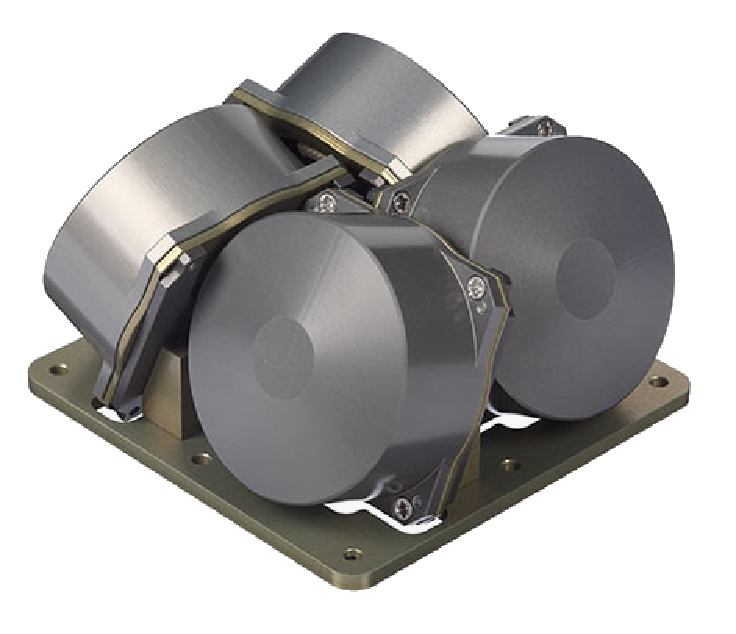
\includegraphics[width=0.5\linewidth]{figures/SatBus-4RW0-1-new.pdf}
    \caption{NanoAvionics (4RW0) integral four - reaction wheels redundant 3-axis control system  }
    \label{fig:na4RW0}
\end{figure}

\noindent Large spacecraft typically used in human spaceflight missions requires large and fast attitude maneuvers, this large demand torque requirement is generally achieved using reaction thrusters. Spacecrafts such as Apollo, Soyuz reentry vehicle used thruster-based \acrshort{acs}. Most recently SpaceX Dragon capsule is equipped with 16 DRACO thrusters \cite{web:SpaceXDargon} for orbit and attitude adjustment capable of producing 400N thrust each.\cite{book:SPACEX} Although being capable of producing large amount of control torques, mission life is limited by finite amount of fuel moreover exhaust fumes may have adverse effects on payload.
\newacronym{ladee}{LADEE}{Lunar Atmosphere and Dust Environment Explorer}
\newacronym{rw}{RW}{Reaction Wheel}
\newacronym{mw}{RW}{Reaction Wheel}
\newacronym{ipacs}{IPACS}{Integrated Power Attitude Control System}

For long duration missions having no possible means of refueling and high pointing accuracy requirements such as Hubble, Kepler Telescopes or optical communication demonstrator like \acrfull{ladee}, Momentum Exchange devices such as \acrfull{rw} or \acrfull{mw} are employed. Perhaps only difference is RWs are at rest at the beginning of mission, whereas MWs are spinning at maximum speed giving gyroscopic stiffness to spacecraft.
Reaction Wheels are used for \acrshort{acs}. Reaction Wheel is a momentum storage device consist of high inertia flywheel attached to an electric brush-less motor with its spin axis kept constant and aligned with spacecraft body. Torque is produced around axis of rotation by changing spin speed of flywheel, since total angular momentum of spacecraft must be conserved, spacecraft counter rotates proportionally to inertia ratio of body and reaction wheel. Very small and precise torques are produced by accelerating flywheels. Satellites are equipped with at least three reaction wheels are required to have complete attitude control capability some use four reaction wheels configuration for redundancy in case of failure as shown in Figure \ref{fig:na4RW0}. Excess energy produced by solar panels during exposure to sun can be stored in RW by means of momentum hence also known as mechanical batteries. Momentum Wheels can be used for both attitude control and mechanical batteries by incorporating \acrfull{ipacs}. \cite{TsiotrasPowerTracking} 

Apart from being very quick and precise internal torque production capabilities Reaction Wheels are limited by maximum angular momentum storage capacity and undergoes saturation. Inability to counteract disturbances on reaching maximum speed is major drawback and thus Reaction wheels must be used with other external torque-based actuators for de-saturation. For large satellites, thruster-based \acrshort{acs} is used for denaturation whereas small satellites often equipped with Magneto Torquers. Current passed through coil of electromagnet attached to spacecraft which creates magnetic dipole. Produced torque is vector product of ambient magnetic flux density vector and magnetic dipole of electromagnet.

Spinning mass has inherent tendency to maintain its axis of rotation. If spin axis is tilted a torque is observed transverse to spin and tilt axis this phenomenon is known as gyroscopic couple. A Control Moment Gyroscope is momentum exchange device consist of a flywheel and one or two motorized gimbles to tilt its spin axis. Flywheel spinning at high angular velocity, hence having high angular momentum. Large "torque amplification" caused by gyroscopic effect produced due to changing orientation of flywheel spin axis is vector cross product of angular momentum of flywheel and velocity of gimble axis rotation.\cite{Leve2015} CMGs are more power efficient than MWs since maintaining wheel spin requires small amount of power. CMGs are classified in two main categories based on number of degrees of freedom of RW spin axis. Single Gimble Control Moment Gyroscope (SGCMG) has one motorized gimble whereas Double Gimble Control Moment Gyroscope (DGCMG) incorporates two gimbles to tilt spin axis of flywheel. SGCMGs are more power efficient than DGCMG since to produce same amount of torque DGCMG requires more electric power. DGCMGs are heavier, requires complex electromechanical components to drive three nested motors. Only advantage of DGCMG is when momentum storage is primary requirement. As size of reaction wheel increased the complexity of DGCMG and its support mechanism keeps increasing due to extra gimble and it becomes no longer feasible. It is also important to avoid alinement of two axis to prevent gimble lock.\cite{ Markley2014} 

One of the earliest research related to use of control moment gyroscope as secondary actuator for gravity gradient stabilize satellite dates to 1964, CMG can act as both actuator and gyro sensor to sense vehicle rates.\cite{Scott1964} Liska proposed torque amplification of several hundred to one by incorporating two independent DGCMGs for 0.01arc sec pointing accuracy with coning type gimble suspension for gimbal synchronization.\cite{Liska1968}
NASA's Marshall Space Flight Center developed manned space station Skylab launched in 1976 was first spacecraft to use CMG for ACS.\cite{SELTZERSM} Software-determined attitude determination to provide general maneuvering ability achieved by making shift from analog controller to fully digital processing system. \cite{Coon1976} First test of USSR CMG also referred as gyrodyne by Russian cosmonauts’ dates to 1974 onboard Salut-3, and standard ACS component for Salut 6 and later missions. Configuration of six SGCMG were used in USSR Mir spacecraft. \cite{Branets1988} Largest DGCMG ever used are installed on International Space Station (ISS) can produce torque up to 258Nm and acts as stations primary attitude control, thrusters are backup for large attitude maneuvers.\cite{Gurrisi2010} 

\newacronym{gs}{GS}{Gain scheduled}
\newacronym{svd}{SVD}{Singular Value Decomposition}
Although CMGs can produce large torque amplification they come with inherent problem of singularity. Phenomenon of inability to provide torque in certain direction based on orientation of flywheel spin axis. Singularity problem can be avoided by adding capability to change the spin speed of flywheel. Avoiding or escaping singular states is possible with added extra degree of freedom of reaction wheel speed hence called Variable Speed Control Moment Gyroscopes a Reaction Wheel mounted on gimble motor. In addition to gyroscopic torques VSCMG produces torque by changing reaction flywheel speed. Direction of torque vector is dependent of orientation of wheel spin axis and gimble motion. Various numerical and geometrical steering approaches are demonstrated for singularity avoidance. Such as Gain scheduled steering and control \cite{SASAKI2017} Singular Value Decomposition (SVD) based gimble speed planning of the transient process \cite{Huang2016}., Robust pseudo inverse method and null motion. Nonlinear Model predictive control realized by Wu. et al. on two VSCMG in scissor pair configuration.  Capability to modulate angular momentum of flywheel can be used to store energy in the form of angular momentum. Yoon, et al. discussed special control algorithm \acrfull{ipacs} on VSCMG cluster. \cite{Yoon2002}. Instead of computing pseudo inverse, Jacobian transpose method can be used for VSCMG stearing. \cite{ KRISHNAN1996431} Quang et al. investigated $\theta-D$ controller with nonlinear state dependent factorization modeling. This adaptive controller is robust in case of \acrshort{rw} failure. \cite{LamThetaD}

A heuristic based inverse kinematics method Forward and Backward Reaching Inverse Kinematics for steering of control moment gyroscope proposed by Meldrom, et al. gives approximate but computationally less expensive results.\cite{MELDRUM2018}
\\

\noindent F. Santoni in 1996 proposed use of neural network trained with optimal nonlinear guidance function, sub-optimal neural network is used to reduce CPU load and memory storage \cite{Santoni1996}. Machine Learning based models are widely used in classification probability prediction problems of finite discrete domain. Recent advancement in reinforcement learning and increased computational performance of microcomputers paved way to solve search problems with large domain. Reinforcement Learning is way of model training a where Agent learns the policy by interacting with environment. Each action performed by agent based on observation in environment has reward associated with it. Optimum policy is having maximum reward. OpenAI Five trained with 2 million frames per 2 seconds leveraging reinforcement learning technique defeated world champions in highly complex real time strategy e-sport game Dota 2.\cite{openai2019dota}. Although, reinforcement learning is not limited to discrete deterministic environment. Real life robotics control problems are nonlinear in nature and require complex steering and control method, problem is continuous, has infinite search space non-deterministic environment. OpenAI trained neural network to solve a Rubik’s cube with a human like robotic hand manipulator, Automatic Domain Randomization is used for training. The model is capable of handling disturbances which had never introduced during training process. \cite{openai2019solving}\\

\newacronym{hil}{HIL}{Hardware in Loop}
\noindent%\subsection{\acrfull{acs} test bench}
Various VSCMG attitude dynamics test bench has been implemented.  Candinia and Santoni manufactured miniature test bed with two axis free moment provided by air bearing and mass balancing around center of gravity is achieved using automatically by using linear actuators. \cite{Candinia2012} Gui et al. talk about testbed with free attitude motion is achieved using spherical air bearing \cite{Gui2015}. Vishvanath et al. deal with design of miniature VSCMG for cubesat, attitude sensors of smartphones are used for state estimation with independent low cost 8bit microcontroller for attitude a control.\cite{2015arXiv150903677P}  Although most of the commercially available attitude control test beds uses air bearing. Air bearing are difficult to manufacture and expensive for sufficiently low friction requirements.
Lorenzo Arena et al. produced a research on use of platform balancing on sharp pinpoint with its center of mass kept close to pivot. Outrunner brushless motors are used since their inertia is sufficient and does not require additional flywheel assembly, research demonstrate FPGA based design for fault tolerant application. \cite{doi:10.1061/(ASCE)AS.1943-5525.0000754}


\newacronym{rl}{RL}{Reinforecement Learning}
%\subsection{\acrfull{rl}}


\section{Thesis Outline}
Scope of this thesis is divided in three parts. First part deals with Mathematical Background. Starting from formulation kinematics and rigid body dynamics, reference frame and axis definition of CMG and complete nonlinear model \acrshort{vscmg} is realized in \autoref{chap:2}. Singularity analysis, momentum envelope and singular surface of \acrshort{vscmg} is discussed in \autoref{chap:3}. Controller design, Lyapunov stability analysis and pseudo inverse based steering law is derived in \autoref{chap:4}. Finally, computer simulations performed for preliminary verification of control algorithm and sizing of hardware component.\\


\noindent Second part of this thesis is discussion of AI based controller methods, Neural Network and Reinforcement Learning. Machine learning approach especially Deep Neural Network and policy gradient training algorithms are discussed in \autoref{chap:5}. Complete policy has been implemented and verified on simulation of spacecraft with VSCMG.\\

\noindent Mechanical Design, Fabrication and electronics and embedded system for hardware in Loop simulation of complete VSCMG Test Bench is implemented in third part of thesis described in \autoref{chap:6} to \autoref{chap:9}.


%\part{Fundamentals}
% Equation of Motion
\chapter{Equation(s) of Motion}
\label{chap:2}
This chapter elaborates selection of reference system, mathematical definition and generalized nonlinear equations of motion of a rigid spacecraft equipped with array of SGCMG units. First inertial and body fixed \ reference frames assigned to individual components and rotation among frames is defined. Right hand rule is followed for representing  rotation of axis in three dimensional space throughout the thesis considering thumb is pointing towards axis of rotation and direction of rotation along curled fingers.Afterwords, inertia property of individual components, their assembly and its derivative is formulated. Later angular momentum of each rotating body is evaluated. Finally, equation of motion is realized for rigid body spacecraft with generic number of SGCMG modules. 

\section{Frame of reference}
To realize attitude of rigid body and its evaluation over time as function of initial angular velocity and applied torques, reference frames and rotation among reference needs to be introduced. We attach body frame $ \mathcal{F}_{b}$ having basis vectors $ (\hat{b}_{1} ,\hat{b}_{2} ,\hat{b}_{3})$ and the orientation of $ \mathcal{F}_{b}$ with respect to inertial reference frame $ \mathcal{F} i$ associated basis vector $ (\hat{e}_{1} ,\hat{e}_{2} ,\hat{e}_{3})$ describes attitude of spacecraft. Rotation from one frame of reference to other can described with Rotation matrix, Euler axis angles representation, Davenport chained rotations, and unit quaternions.

\subsection{Rotation Matrix}
Three mutually perpendicular basis vectors describes reference frame in Euclidean space. Rotation is represented by specifying vector components of one frame with respect to other. Each column describe components of unit vector.
\begin{equation}
\mathbf{R}_{3\times 3} \ =\ \begin{pmatrix}
\vdots  & \vdots  & \vdots \\
\hat{e}_{1} & \hat{e}_{2} & \hat{e}_{3}\\
\vdots  & \vdots  & \vdots 
\end{pmatrix}
\end{equation}

\begin{equation}
\begin{aligned}
\mathbf{R}^{T}\mathbf{R} =\mathbf{RR}^{T} =\mathbf{I}_{3\times 3}\\
\det\mathbf{R} =+1
\end{aligned}
\label{eqn:rotmat}
\end{equation}

$ R$ is real and orthogonal matrix with eigenvalues $ \left\{1,e^{\pm i\theta }\right\}$, with unit determinant. Successive rotations are represented as product of matrix in order of rotation performed.


\begin{equation}
^{B}\mathbf{R}_{I} =\ ^{B}\mathbf{R}_{n} \ ^{n}\mathbf{R}_{n-1} \cdots ^{2}\mathbf{R}_{1} \ ^{1}\mathbf{R}_{I}
\end{equation}

\subsection{Euler Axis angle}

Euler rotation theorem states If $ \mathbf{R}$ satisfies \autoref{eqn:rotmat} then there exist non zero vector $ \hat{\mathbf{a}}$ which satisfies $ \mathbf{R\hat{a}} =\hat{\mathbf{a}}$. Any arbitrary composition of rotations of a rigid body can be represented as single rotation by angle $ \varphi $ about unique axis $ \hat{\mathbf{a}}$ which remains unchanged by the rotation.\cite{eulerAxis} Rotation matrix $ \mathbf{R}$ relates certain vector $ \mathbf{v}$ and corrusponding rotated vector $ \mathbf{v'} =\mathbf{Rv}$ Roudrigues rotation formula for $ \mathbf{R}$ as function of unit vector $ \hat{\mathbf{a}}$ along the rotation axis and by angle $ \varphi $ is
\begin{equation}
\mathbf{R}(\hat{\mathbf{a}} ,\varphi ) =\cos \varphi \ \mathbf{I} \ +\ ( 1-\cos \varphi ) \ \hat{\mathbf{a}} \otimes \hat{\mathbf{a}} +\sin( \varphi ) \ \hat{\mathbf{a}}^{\times }
\end{equation}
Here $\mathbf{I}$ is identity matrix and vector with superscript $\times$ is a skew symmetric matrix equivalent for cross product of vector, commonly referred as "Hat-Map" transformation denoted with $a^{\times}$ represented as

\begin{equation*}
a^{\times } =\begin{pmatrix}
0 & -a_{3} & a_{2}\\
a_{3} & 0 & -a_{1}\\
-a_{2} & a_{1} & 0
\end{pmatrix}
\end{equation*}
With dextro-rotation assumption, $ \mathbf{R}$ moves the vectors but not co-ordinate axes hence gives active point of view of rotation.

\subsection{Davenport chained rotations}
Davenport chained rotations are three chained sequence of consecutive intrinsic rotation about body-fixed axes. Based on number of axes used to represent rotation Davenport chain rotations are characterized in two types, "Generalized Euler rotations" if two rotation occurs about same axis and "Generalized Tait–Bryan rotations" if each rotations occur about different axis. Order in which rotations are performed is not cumulative so must be specified. Three numbers indicates axis about which rotations are performed. For example Euler 313 commonly used in aerodynamics to describe satellites position with other parameters. Sequence involves first rotation about third axis, second rotation about first axis and finally, third rotation about third axis. Tait-Bryan angle sequence 123 is commonly used t describe attitude of aircraft and individual rotation is called roll, pitch and yaw ($ \phi ,\theta ,\psi $). Classic Euler angles are first introduced by Euler for orbital mechanics and rigid body dynamics. Problem with classic Euler angle is, they become singular near zero angles, on the other hand Tait–Bryan angles become singular when second rotation is $ \pi/2$ condition also referred as Gimble Lock. \\

\noindent Elaboration of Tait–Bryan $ R_{123}$ is product of three individual coordinate rotation about each axis$ R_{i} :\mathbb{R}\longrightarrow SO( 3)$ for $ i\in \{1,2,3\}$ as shown below:


\begin{equation*}
R_{1} (\phi )=\begin{pmatrix}
1 & 0 & 0\\
0 & \cos \phi  & \sin \phi \\
0 & -\sin \phi  & \cos \phi 
\end{pmatrix}
\end{equation*}
\begin{equation*}
R_{2} (\theta )=\begin{pmatrix}
\cos \theta  & 0 & -\sin \theta \\
0 & 1 & 0\\
\sin \theta  & 0 & \cos \theta 
\end{pmatrix}
\end{equation*}
\begin{equation*}
R_{3} (\psi )=\begin{pmatrix}
\cos \psi  & \sin \psi  & 0\\
-\sin \psi  & \cos \psi  & 0\\
0 & 0 & 1
\end{pmatrix}
\end{equation*}
Performing the multiplication, the complete rotation from the body frame to the inertial frame is given by
\begin{equation*}
    R_{123}( \phi ,\theta ,\psi ) =R_{1} (\phi )R_{2} (\theta )R_{3} (\psi )
\end{equation*}
\begin{equation*}
R_{123} (\phi ,\theta ,\psi )=
\end{equation*}
\begin{equation*}
    \begin{pmatrix}
\cos \psi \cos \theta  & \cos \psi \sin \phi \sin \theta -\cos \phi \sin \psi  & \sin \phi \sin \psi +\cos \phi \cos \psi \sin \theta \\
\cos \theta \sin \psi  & \cos \phi \cos \psi +\sin \phi \sin \psi \sin \theta  & \cos \phi \sin \psi \sin \theta -\cos \psi \sin \phi \\
-\sin \theta  & \cos \theta \sin \phi  & \cos \phi \cos \theta 
\end{pmatrix}
\end{equation*}

\subsection{Quaternions}
Quaternions were introduced by William Rowan Hamilton as four dimension vector having three imaginary dimensions describing space and a real number perpendicular to it in fourth dimension. Quaternion rotation is written as combination of scalar with hyper-complex numbers \ in the form of 


\begin{equation}
\mathbf{q} =q_{0} \ +\ q_{1}\mathbf{i} \ +q_{2} \ \mathbf{j} \ +q_{3} \ \mathbf{k}
\end{equation}
where $\displaystyle \{q_{0} ,q_{1} ,q_{2} ,q_{3}\} \ \in \ \mathbb{R}$ and $\displaystyle i,j,k$ are the fundamental quaternion units. Hamiltonian representation of quaternion follows \footnote{Apart from Hamiltonian representation, an alternative standard representation "JPL" \cite{Ortega2016QuaternionKF} has component order as $q=q_0i+q_1j+q_2k+q_3$ holds algebraic relation 
$\mathbf{i}^{2} +\mathbf{j}^{2} +\mathbf{k}^{2} =\mathbf{ijk} =1$}
\begin{equation}
\mathbf{i}^{2} +\mathbf{j}^{2} +\mathbf{k}^{2} =\mathbf{ijk} =-1
\end{equation}
The term $\displaystyle \mathbf{i} ,\mathbf{j} ,\mathbf{k}$ represents three unit Cartesian with imaginary properties and satisfies following relation
\begin{gather*}
\mathbf{ij} =\mathbf{k} \ \quad \mathbf{ij} =-\mathbf{k}\\
\mathbf{jk} =\mathbf{i} \ \quad \mathbf{jk} =-\mathbf{i}\\
\mathbf{ki} =\mathbf{j} \ \quad \mathbf{ki} =-\mathbf{j}
\end{gather*}
A quaternion $\displaystyle \mathbf{q} \in \mathbb{H}$ is represented as vector with scalar $\displaystyle q_{0}$ and $\displaystyle \mathbf{q_v} =[ q_{1} \ q_{2} \ q_{3}]^{T}$as


\begin{equation*}
\mathbf{q} =\begin{bmatrix}
q_{0} & q_{1} & q_{2} & q_{3}
\end{bmatrix}^{T} =\begin{bmatrix}
q_{0}\\
\mathbf{q_v}
\end{bmatrix}
\end{equation*}
Quaternion norm conjugate and inverse is computed as


\begin{gather}
\mathbf{q}^{*} =\begin{bmatrix}
q_{0}\\
-\mathbf{q}
\end{bmatrix} \ \\
\| \mathbf{q} \| =\sqrt{\mathbf{qq}^{*}} =\sqrt{q^{2}_{0} +q^{2}_{1} +q^{2}_{2} +q^{2}_{3}}\\
\mathbf{q}^{-1} =\frac{\mathbf{q}^{*}}{\| \mathbf{q} \| ^{2}}
\end{gather}
Quaternion product is noncommutative, defined in terms of scalar and vector part, product of two quaternion $\displaystyle \mathbf{q}_{1}$ and $\displaystyle \mathbf{q}_{2}$ evaluated as 
\begin{equation}
\label{quatProduct}
\begin{aligned}
\mathbf{q_{1} \otimes q_{2}} & =\begin{bmatrix}
q_{1,0}\\
q_{1,v}
\end{bmatrix} \otimes \begin{bmatrix}
q_{2,0}\\
{\mathbf{q}_{2,v}}
\end{bmatrix}\\
 & =\ \begin{bmatrix}
q_{1,0} q_{2,0} - q_{1,v} \cdot q_{2,v}\\
q_{1,0} q_{2,v} +q_{2,0} q_{1} +\mathbf{q ^{\times }_{1} q}_{2,v}
\end{bmatrix}
\end{aligned} \ 
\end{equation}
Unit quaternions are special class of quaternion which poses following property
\begin{equation}
\| \mathbf{q} \| =\sqrt{q^{2}_{0} +q^{2}_{1} +q^{2}_{2} +q^{2}_{3}} =1
\end{equation}
Rotation in three dimensions can be represented with unit quaternions, they have been employed in several disciplines such as computer graphics, aerodynamics, quantum computing, robotics and to describe attitude of rigid body. \ Consider a vector $\displaystyle \mathbf{x} \in \mathbb{R}^{3}$ in inertial frame $\displaystyle \mathcal{F}_{i}$ and $\displaystyle \mathbf{x} '$ being same vector viewed from body fixed frame then we get rotation of vector $\displaystyle \mathbf{x}$ as
\begin{equation*}
\begin{aligned}
\begin{bmatrix}
0\\
\mathbf{x} '
\end{bmatrix} & =\mathbf{q} \cdot \begin{bmatrix}
0\\
\mathbf{x}
\end{bmatrix} \cdot \mathbf{q}^{-1}\\
 & =\begin{bmatrix}
1 & \mathbf{0}^{T}\\
\mathbf{0} & \mathbf{R}(\mathbf{q})
\end{bmatrix}\begin{bmatrix}
0\\
\mathbf{x} '
\end{bmatrix}\\
\mathbf{x} ' & =\mathbf{R}(\mathbf{q})\mathbf{x}\\
\mathbf{x} & =\mathbf{R}(\mathbf{q})^{T}\mathbf{x} '
\end{aligned}
\end{equation*}
where rotation matrix $\displaystyle \mathbf{R}$ as function of $\displaystyle \mathbf{q}$ shown below.
\begin{equation}
\ \begin{aligned}
\mathbf{R}(\mathbf{q}) & =\left( q^{2}_{0} -\mathbf{q_v ^{T} q_v}\right)\mathbf{I}_{3\times 3} +2\mathbf{q_v q_v}^{T} +2q_{0}\mathbf{q}^{\times }\\
\mathbf{R}(\mathbf{q}) & =\begin{pmatrix}
1-2q^{2}_{2} -2q^{2}_{3} & 2q_{1} q_{2} -2q_{0} q_{3} & 2q_{1} q_{3} +2q_{0} q_{2}\\
2q_{1} q_{2} +2q_{0} q_{3} & 1-2q^{2}_{1} -2q^{2}_{3} & 2q_{2} q_{3} -2q_{0} q_{1}\\
2q_{1} q_{3} -2q_{0} q_{2} & 2q_{2} q_{3} +2q_{0} q_{1} & 1-2q^{2}_{1} -2q^{2}_{2}
\end{pmatrix}
\end{aligned}
\end{equation}
Relation ship with axis angle $\displaystyle \hat{\mathbf{e}} =[ e_{1} \ e_{2} \ e_{3}]^{T}$ and rotation by angle $\displaystyle \varphi $ is expressed as follows
\begin{equation}
\label{eqn:axisAngle}
\mathbf{q} =\begin{bmatrix}
\cos\frac{\varphi }{2}\\
\hat{\mathbf{e}} \ \sin\frac{\varphi }{2}
\end{bmatrix}
\end{equation}
Let us write spacecraft attitude quaternion having body fix frame $\displaystyle \mathcal{F}_{b}$ with respect to inertial frame frame $\displaystyle \mathcal{F} i$ as $\displaystyle \mathbf{q}$ and desired attitude in body frame $\displaystyle \mathcal{F}_{d}$ is $\displaystyle \mathbf{q}_{d}$. Magnitude of angular displacement between frame $\displaystyle \mathcal{F}_{b}$ and frame $\displaystyle \mathcal{F}_{d}$ is described by angle $\displaystyle \varepsilon $ by eigenaxis rotation about $\displaystyle \hat{e}$ is error between current and desired attitude attitude $\displaystyle \mathbf{q}_{e} =\left[\mathbf{q}_{e,0} ,\mathbf{q}^{T}_{e,v}\right]^{T}$.
\begin{equation*}
\mathbf{q_{d} q}_{e} =\mathbf{q}
\end{equation*}
premultyplying by conjugate $\displaystyle \mathbf{q}^{*}_{d}$, we get error quaternion.
\begin{equation*}
\mathbf{q}_{e} =\mathbf{q^{*}_{d} q}
\end{equation*}
\begin{equation}
\begin{pmatrix}
\mathbf{q}_{e,0}\\
\mathbf{q}_{e,v}
\end{pmatrix} =\begin{pmatrix}
\cos( \varepsilon /2) \ \\
\mathbf{\hat{e}}\sin( \varepsilon /2)
\end{pmatrix} =\begin{pmatrix}
q_{0} q_{d,0} +\mathbf{q}^{T}\mathbf{q}_{d}\\
-q_{0}\mathbf{q}_{d,v} +q_{d,0}\mathbf{q_{v}} -\mathbf{q_{d,v}} \times \mathbf{q}_{v}
\end{pmatrix}
\end{equation}
\section{Kinematics}
Kinematic relation of rigid body describes changing attitude over time of body fixed reference frame $\displaystyle \mathcal{F}_{b}$ with inertial reference frame $\displaystyle \mathcal{F}_{i}$.To identify kinematic differential equation, let us consider instantaneous angular velocity vector $\displaystyle \mathbf{\omega }$ of frame $\displaystyle \mathcal{F}_{b}$ with respect to frame $\displaystyle \mathcal{F} i$ as viewed from $\displaystyle \mathcal{F}_{b}$ frame orthogonal components described as
\begin{equation*}
\mathbf{\omega } =\omega_{1}\hat{\mathbf{b}}_{1} +\omega_{2}\hat{\mathbf{b}}_{2} +\omega_{3}\hat{\mathbf{b}}_{3}
\end{equation*}
Then $\displaystyle ^{\mathcal{F}_{i}} d/dt\{\hat{\mathbf{b}}\}$ is derivative of $\displaystyle \mathcal{F}_{b}$ base vectors taken in $\displaystyle \mathcal{F} i$, applying transport theorem
\begin{equation}
\frac{^{\mathcal{F}_{i}} d}{dt} \ \hat{\mathbf{b}}_{i} =\ \frac{^{\mathcal{F}_{b}} d}{dt} \ \hat{\mathbf{b}}_{i} +\ \mathbf{\omega } \times \ \hat{\mathbf{b}}_{i}
\end{equation}
Selection of attitude coordinate system to represent rotation of spacecraft is crucial in order to simplify mathematics and avoid geometrical or numerical singularity, quaternion kinematics is used in this thesis. In spite of the fact that quaternions are less intuitive, they does not undergo trivial singularity \ presence in Euler angles moreover quaternions are linear in nature. In this section we will realize quaternion kinematic relation.

Let $\displaystyle \mathbf{q}$ represent attitude of spacecraft with respect to inertial reference frame at time $\displaystyle t$ and $\displaystyle \mathbf{q}$' be attitude quaternion after $\displaystyle t+\Delta t$ about axis $\displaystyle \hat{\mathbf{e}}$ and by angle $\displaystyle \Delta \varphi $ rotation using \autoref{eqn:axisAngle}
\begin{equation}
\dot{\mathbf{q}} =\mathbf{q}( t+\Delta t) =\mathbf{q} '=\begin{bmatrix}
\cos\frac{\Delta \varphi }{2}\\
\hat{\mathbf{e}} \ \sin\frac{\Delta \varphi }{2}
\end{bmatrix}
\end{equation}
amusing very small angle $\displaystyle \Delta \varphi =\mathbf{\omega } \Delta t$ thus $\displaystyle \cos\frac{\Delta \varphi }{2} \approx 1$ and $\displaystyle \sin\frac{\Delta \varphi }{2} \approx \frac{\Delta \varphi }{2}$
\begin{equation}
\begin{aligned}
\dot{\mathbf{q}} & =\frac{1}{2}
\begin{bmatrix}
-\mathbf{\omega } \cdot \mathbf{q}\\
 q_{0}\mathbf{\omega } -\mathbf{q}^{\times }
\end{bmatrix}\\
 & =\frac{1}{2}\begin{bmatrix}
0 & -\mathbf{\omega^T }\\
\mathbf{\omega } & -\mathbf{\omega }^{\times }
\end{bmatrix}\begin{bmatrix}
q_{0}\\
\mathbf{q}
\end{bmatrix}
\end{aligned}
\end{equation}
Considering constant angular velocity for small time step evaluation in body frame a quaternion kinematics equation for rigid body derived as follows.
\begin{equation}
\dot{\mathbf{q}} =\frac{1}{2}\begin{pmatrix}
0 & -\omega^b_{1} & -\omega^b_{2} & -\omega^b_{3}\\
\omega^b_{1} & 0 & -\omega^b_{3} & \omega^b_{2}\\
\omega^b_{2} & \omega^b_{3} & 0 & -\omega^b_{1}\\
\omega^b_{3} & -\omega^b_{2} & \omega^b_{1} & 0
\end{pmatrix}\begin{pmatrix}
q_{0}\\
q_{1}\\
q_{2}\\
q_{3}
\end{pmatrix}
\end{equation}
As seen from inertial frame quaternion derivative in terms of angular velocity can be evaluated by
\begin{equation*}
\omega^i =\mathbf{q}^{*}\mathbf{\omega^i \ q} \ \quad or\ \mathbf{\quad \omega^b } =\mathbf{q}^{*}\mathbf{\omega^b \ q}
\end{equation*}
\begin{equation}
\dot{\mathbf{q}} =\frac{1}{2}\mathbf{\omega^i }(\mathbf{\omega^b })\mathbf{q} =\frac{1}{2}\begin{pmatrix}
0 & -\omega^i_{1} & -\omega^i_{2} & -\omega^i_{3}\\
\omega^i_{1} & 0 & \omega^i_{3} & -\omega^i_{2}\\
\omega^i_{2} & -\omega^i_{3} & 0 & \omega^i_{1}\\
\omega^i_{3} & \omega^i_{2} & -\omega^i_{1} & 0
\end{pmatrix}\begin{pmatrix}
q_{0}\\
q_{1}\\
q_{2}\\
q_{3}
\end{pmatrix}
\end{equation}
Since no analytical simulation exists for changing angular velocity, kinematics is integrated numerically using Adaptive Runge–Kutta method.
 
\clearpage
\section{Dynamics}
In order to archive complete system dynamics of spacecraft with array of N - VSCMGs, physical properties such as inertia and angular momentum of a single control moment gyroscope is evaluated first and latter for arrangement of spacecraft with multpile VSCMG units . Body fixed frame $\displaystyle \mathcal{F}_{b}$with basis vector $\displaystyle \{\hat{b}_{1} ,\hat{b}_{2} ,\hat{b}_{3}\}$ attached to center of mass of continuum rigid body at distance $\displaystyle \vec{r}_{0}$ from $\displaystyle \mathcal{F}_{i}$ as shown in \autoref{fig:tikRigidBody}. Body is rotating at angular velocity $\displaystyle \vec{\omega } =[ \omega _{1} \ \omega _{2} \ \omega _{3}]^{T}$ as shown in fig. The angular momentum $\displaystyle \delta \vec{\mathbf{h}}$ of infinitesimally small mass $\displaystyle \delta m$ at position $\displaystyle \vec{r} =[ x_{1} \ y_{2} \ z_{3}]^{T}$ in body, moving at velocity $\displaystyle \mathbf{\vec{v}} =\vec{\mathbf{\omega }} \times \vec{r}$ is expressed as
\begin{equation*}
\delta \vec{\mathbf{h}} =\ \vec{r} \times \delta m\mathbf{\vec{v}}
\end{equation*}
\begin{figure}[!ht]
    \centering
    

\tikzset{every picture/.style={line width=0.75pt}} %set default line width to 0.75pt        

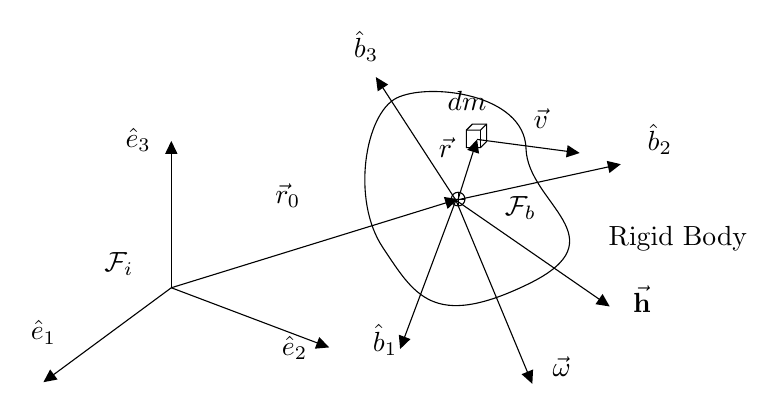
\begin{tikzpicture}[x=0.75pt,y=0.75pt,yscale=-1,xscale=1]
%uncomment if require: \path (0,197); %set diagram left start at 0, and has height of 197

%Straight Lines [id:da6848421575573145] 
\draw    (220.55,133.73) -- (161.35,177.43) ;
\draw [shift={(158.93,179.22)}, rotate = 323.56] [fill={rgb, 255:red, 0; green, 0; blue, 0 }  ][line width=0.08]  [draw opacity=0] (6.25,-3) -- (0,0) -- (6.25,3) -- cycle    ;
%Straight Lines [id:da9130919810329883] 
\draw    (220.55,133.73) -- (220.55,65.99) ;
\draw [shift={(220.55,62.99)}, rotate = 450] [fill={rgb, 255:red, 0; green, 0; blue, 0 }  ][line width=0.08]  [draw opacity=0] (6.25,-3) -- (0,0) -- (6.25,3) -- cycle    ;
%Straight Lines [id:da6717502672065161] 
\draw    (220.55,133.73) -- (293.81,161.42) ;
\draw [shift={(296.61,162.48)}, rotate = 200.71] [fill={rgb, 255:red, 0; green, 0; blue, 0 }  ][line width=0.08]  [draw opacity=0] (6.25,-3) -- (0,0) -- (6.25,3) -- cycle    ;
%Shape: Polygon Curved [id:ds602562353451706] 
\draw   (329.07,42.33) .. controls (344.28,34.72) and (390.68,40.05) .. (391.44,66.67) .. controls (392.2,93.29) and (437.84,110.03) .. (392.2,132.09) .. controls (346.56,154.15) and (337.59,137.03) .. (322.37,114.21) .. controls (307.16,91.39) and (313.85,49.94) .. (329.07,42.33) -- cycle ;
%Straight Lines [id:da39324245591715457] 
\draw    (357.65,91.54) -- (331.83,160.45) ;
\draw [shift={(330.78,163.26)}, rotate = 290.54] [fill={rgb, 255:red, 0; green, 0; blue, 0 }  ][line width=0.08]  [draw opacity=0] (6.25,-3) -- (0,0) -- (6.25,3) -- cycle    ;
%Straight Lines [id:da930908309847323] 
\draw    (357.65,91.54) -- (320.74,34.74) ;
\draw [shift={(319.1,32.22)}, rotate = 416.98] [fill={rgb, 255:red, 0; green, 0; blue, 0 }  ][line width=0.08]  [draw opacity=0] (6.25,-3) -- (0,0) -- (6.25,3) -- cycle    ;
%Straight Lines [id:da12681885554956018] 
\draw    (357.65,91.54) -- (434.17,74.84) ;
\draw [shift={(437.1,74.2)}, rotate = 527.69] [fill={rgb, 255:red, 0; green, 0; blue, 0 }  ][line width=0.08]  [draw opacity=0] (6.25,-3) -- (0,0) -- (6.25,3) -- cycle    ;
%Shape: Cube [id:dp2442226204871445] 
\draw   (362.69,57.8) -- (365.61,54.88) -- (372.43,54.88) -- (372.43,63.32) -- (369.5,66.24) -- (362.69,66.24) -- cycle ; \draw   (372.43,54.88) -- (369.5,57.8) -- (362.69,57.8) ; \draw   (369.5,57.8) -- (369.5,66.24) ;
%Straight Lines [id:da1664531723187539] 
\draw    (220.55,133.73) -- (355.87,91.9) ;
\draw [shift={(358.73,91.01)}, rotate = 522.8199999999999] [fill={rgb, 255:red, 0; green, 0; blue, 0 }  ][line width=0.08]  [draw opacity=0] (6.25,-3) -- (0,0) -- (6.25,3) -- cycle    ;
%Straight Lines [id:da786199273063587] 
\draw    (357.65,91.54) -- (393.33,177.24) ;
\draw [shift={(394.48,180.01)}, rotate = 247.4] [fill={rgb, 255:red, 0; green, 0; blue, 0 }  ][line width=0.08]  [draw opacity=0] (6.25,-3) -- (0,0) -- (6.25,3) -- cycle    ;
%Straight Lines [id:da5324752074176795] 
\draw    (357.65,91.54) -- (429.29,141.03) ;
\draw [shift={(431.76,142.74)}, rotate = 214.64] [fill={rgb, 255:red, 0; green, 0; blue, 0 }  ][line width=0.08]  [draw opacity=0] (6.25,-3) -- (0,0) -- (6.25,3) -- cycle    ;
%Straight Lines [id:da8372140293451968] 
\draw    (367.86,62.26) -- (414.33,68.41) ;
\draw [shift={(417.3,68.8)}, rotate = 187.54] [fill={rgb, 255:red, 0; green, 0; blue, 0 }  ][line width=0.08]  [draw opacity=0] (6.25,-3) -- (0,0) -- (6.25,3) -- cycle    ;
%Straight Lines [id:da011174792069704065] 
\draw    (358.73,91.01) -- (366.95,65.12) ;
\draw [shift={(367.86,62.26)}, rotate = 467.61] [fill={rgb, 255:red, 0; green, 0; blue, 0 }  ][line width=0.08]  [draw opacity=0] (6.25,-3) -- (0,0) -- (6.25,3) -- cycle    ;
%Flowchart: Or [id:dp557393747624519] 
\draw   (355.44,91.01) .. controls (355.44,89.19) and (356.91,87.72) .. (358.73,87.72) .. controls (360.55,87.72) and (362.03,89.19) .. (362.03,91.01) .. controls (362.03,92.83) and (360.55,94.31) .. (358.73,94.31) .. controls (356.91,94.31) and (355.44,92.83) .. (355.44,91.01) -- cycle ; \draw   (355.44,91.01) -- (362.03,91.01) ; \draw   (358.73,87.72) -- (358.73,94.31) ;

% Text Node
\draw (151.61,148.34) node [anchor=north west][inner sep=0.75pt]    {$\hat{e}_{1}$};
% Text Node
\draw (272.55,155.94) node [anchor=north west][inner sep=0.75pt]    {$\hat{e}_{2}$};
% Text Node
\draw (197.25,55.54) node [anchor=north west][inner sep=0.75pt]    {$\hat{e}_{3}$};
% Text Node
\draw (316.42,150.17) node [anchor=north west][inner sep=0.75pt]    {$\hat{b}_{1}$};
% Text Node
\draw (448.77,53.57) node [anchor=north west][inner sep=0.75pt]    {$\hat{b}_{2}$};
% Text Node
\draw (307.29,8.69) node [anchor=north west][inner sep=0.75pt]    {$\hat{b}_{3}$};
% Text Node
\draw (441.81,131.47) node [anchor=north west][inner sep=0.75pt]    {$\vec{\mathbf{h}}$};
% Text Node
\draw (402.94,165.83) node [anchor=north west][inner sep=0.75pt]    {$\vec{\omega }$};
% Text Node
\draw (393.84,46.28) node [anchor=north west][inner sep=0.75pt]    {$\vec{v}$};
% Text Node
\draw (348.2,59.97) node [anchor=north west][inner sep=0.75pt]    {$\vec{r}$};
% Text Node
\draw (352.45,37.67) node [anchor=north west][inner sep=0.75pt]    {$dm$};
% Text Node
\draw (269.38,82.26) node [anchor=north west][inner sep=0.75pt]    {$\vec{r}_{0}$};
% Text Node
\draw (430,103) node [anchor=north west][inner sep=0.75pt]   [align=left] {Rigid Body};
% Text Node
\draw (187,115.4) node [anchor=north west][inner sep=0.75pt]    {$\mathcal{F}_{i}$};
% Text Node
\draw (380,88.4) node [anchor=north west][inner sep=0.75pt]    {$\mathcal{F}_{b}$};
\end{tikzpicture}

    \caption{Representation of Rigid body rotation in space}
    \label{fig:tikRigidBody}
\end{figure}
Total angular momentum for rigid body is given by
\begin{equation*}
\begin{aligned}
\vec{\mathbf{h}} & =\int _{\mathcal{B}}(\vec{r} \times \mathbf{\vec{v}} \ ) \delta m\\
\vec{\mathbf{h}} & =\int _{\mathcal{B}}[\vec{r} \times (\vec{\mathbf{\omega }} \times \vec{r})] \ \delta m
\end{aligned}
\end{equation*}
Expanding the vector quantities we get
\begin{equation*}
\vec{\mathbf{h}} =h_{1}\hat{\mathbf{e}}_{1} +h_{2}\hat{\mathbf{e}}_{2} +h_{3}\hat{\mathbf{e}}_{3}
\end{equation*}
Thus angular momentum vector in body frame is given by
\begin{equation}
\begin{aligned}
\vec{\mathbf{h}}_{B} & =\mathbf{I\ \omega }_{B}\\
\overrightarrow{\mathbf{h}_{B}} & =\begin{pmatrix}
I_{x} & -I_{xy} & -I_{xz}\\
-I_{y} & I_{y} & -I_{yz}\\
I_{z} & -I_{zy} & I_{z}
\end{pmatrix}\begin{pmatrix}
\omega _{1}\\
\omega _{2}\\
\omega _{3}
\end{pmatrix}
\end{aligned}
\end{equation}
here components of inertia tensor $\displaystyle \mathbf{I}$ are moment of inertia $\displaystyle I_{x} ,I_{y} ,I_{z}$ and product of inertia $\displaystyle I_{xy} ,I_{yz} ,I_{xz}$are


\begin{gather*}
 \begin{aligned}
I_{x} =\int _{\mathcal{B}}\left( y^{2} +z^{2}\right) \delta m; & & I_{y} =\int _{\mathcal{B}}\left( x^{2} +z^{2}\right) \delta m; & & I_{z} =\int _{\mathcal{B}}\left( x^{2} +y^{2}\right) \delta m\\
I_{xy} =\int _{\mathcal{B}}( xy) \delta m; & & I_{xz} =\int _{\mathcal{B}}( xz) \delta m; & & I_{yz} =\int _{\mathcal{B}}( yz) \delta m
\end{aligned} \ \ \\
\end{gather*}
Total rotational kinetic energy is evaluated as:



\begin{equation}
\mathcal{T} =\frac{1}{2}\vec{\mathbf{\omega }} \cdotp \hat{\mathbf{h}} =\frac{1}{2}\vec{\mathbf{\omega }}^{T}_{B} \cdotp \hat{\mathbf{h}}_{B}
\end{equation}


\subsection{System Representation}
Let us consider a generic CMG attached to rigid free floating spacecraft body with respect to inertial frame $\displaystyle \mathcal{F}_{i}$ having basis $\displaystyle \{\hat{e}_{1} ,\hat{e}_{2} ,\hat{e}_{2}\}$ as shown in \autoref{fig:tikSGCMGFrame}. Body frame $\displaystyle \mathcal{F}_{b}$ with basis vector $\displaystyle \{\hat{b}_{1} ,\hat{b}_{2} ,\hat{b}_{2}\}$ is used to represent attitude of spacecraft with respect to \ $\displaystyle \mathcal{F}_{i}$. Another reference frame $\displaystyle \mathcal{F}_{g}$ attached to the center of mass having basis vector $\displaystyle \{\hat{g} ,\hat{s} ,\hat{t}\}$. Gimbal axis is aliened with unit vector $\displaystyle \hat{g}$ and spin axis attached to $\displaystyle \hat{s}$ and orthogonal to gimbal axis. Transverse axis $\displaystyle \hat{t}$ is described as $\displaystyle \hat{t} =\hat{g} \times \hat{s}$ making it mutually perpendicular to $\displaystyle \hat{g}$ and $\displaystyle \hat{s}$. Gimbal motor rotates $\displaystyle \hat{s}$ and $\displaystyle \hat{t}$ with respect to $\displaystyle \mathcal{F}_{b}$

\begin{figure}[!ht]
    \centering
    

\tikzset{every picture/.style={line width=0.75pt}} %set default line width to 0.75pt        

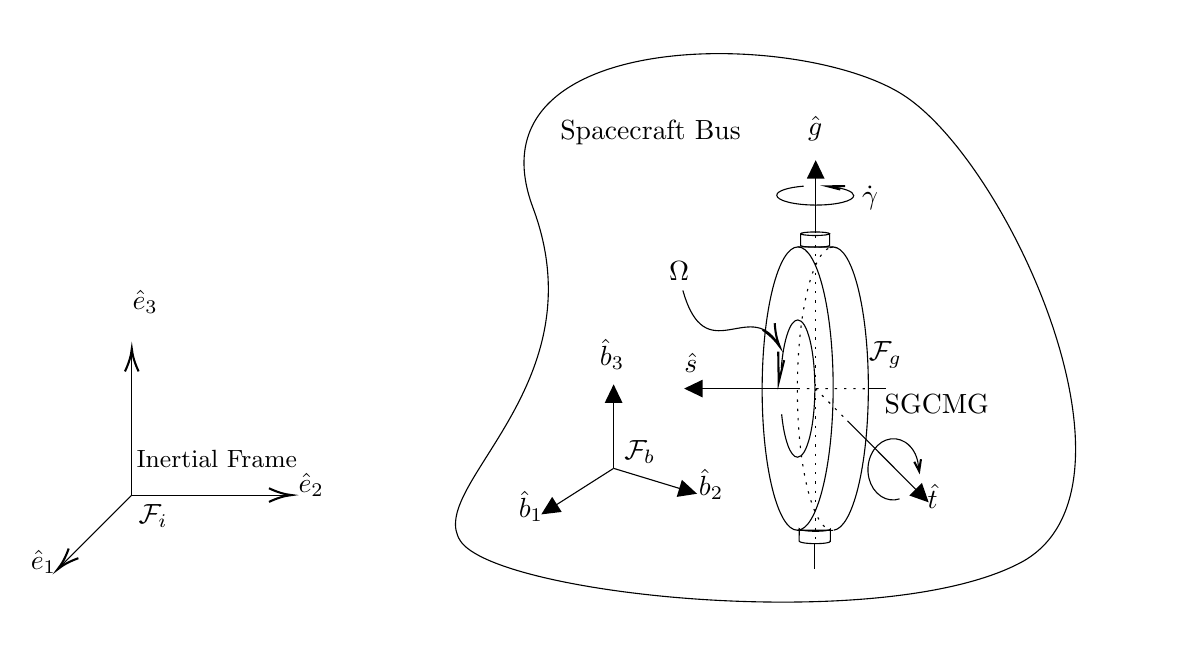
\begin{tikzpicture}[x=0.75pt,y=0.75pt,yscale=-1,xscale=1]
%uncomment if require: \path (0,300); %set diagram left start at 0, and has height of 300

%Straight Lines [id:da892975500466239] 
\draw    (73.1,228.21) -- (38.71,262.6) ;
\draw [shift={(37.3,264.02)}, rotate = 315] [color={rgb, 255:red, 0; green, 0; blue, 0 }  ][line width=0.75]    (10.93,-3.29) .. controls (6.95,-1.4) and (3.31,-0.3) .. (0,0) .. controls (3.31,0.3) and (6.95,1.4) .. (10.93,3.29)   ;
%Straight Lines [id:da5595617967419346] 
\draw    (73.1,228.21) -- (148.13,228.21) ;
\draw [shift={(150.13,228.21)}, rotate = 180] [color={rgb, 255:red, 0; green, 0; blue, 0 }  ][line width=0.75]    (10.93,-3.29) .. controls (6.95,-1.4) and (3.31,-0.3) .. (0,0) .. controls (3.31,0.3) and (6.95,1.4) .. (10.93,3.29)   ;
%Straight Lines [id:da36715700773366944] 
\draw    (73.1,228.21) -- (73.1,159.69) ;
\draw [shift={(73.1,157.69)}, rotate = 450] [color={rgb, 255:red, 0; green, 0; blue, 0 }  ][line width=0.75]    (10.93,-3.29) .. controls (6.95,-1.4) and (3.31,-0.3) .. (0,0) .. controls (3.31,0.3) and (6.95,1.4) .. (10.93,3.29)   ;
%Shape: Ellipse [id:dp29439730581719936] 
\draw   (394.05,108.64) .. controls (384.6,108.62) and (376.88,139.16) .. (376.8,176.85) .. controls (376.72,214.55) and (384.32,245.12) .. (393.76,245.14) .. controls (403.21,245.16) and (410.93,214.62) .. (411.01,176.93) .. controls (411.09,139.23) and (403.5,108.66) .. (394.05,108.64) -- cycle ;
%Shape: Arc [id:dp10136348529454264] 
\draw  [draw opacity=0] (411.29,245.14) .. controls (420.48,243.96) and (427.89,213.89) .. (427.97,176.96) .. controls (428.05,139.27) and (420.45,108.69) .. (411.01,108.67) .. controls (410.47,108.67) and (409.95,108.77) .. (409.43,108.96) -- (410.86,176.93) -- cycle ; \draw   (411.29,245.14) .. controls (420.48,243.96) and (427.89,213.89) .. (427.97,176.96) .. controls (428.05,139.27) and (420.45,108.69) .. (411.01,108.67) .. controls (410.47,108.67) and (409.95,108.77) .. (409.43,108.96) ;
%Shape: Arc [id:dp2890410550496316] 
\draw  [draw opacity=0][dash pattern={on 0.84pt off 2.51pt}] (412.91,109.1) .. controls (412.29,108.82) and (411.65,108.67) .. (411.01,108.67) .. controls (401.56,108.65) and (393.84,139.19) .. (393.76,176.89) .. controls (393.68,213.1) and (400.69,242.74) .. (409.61,245.04) -- (410.86,176.93) -- cycle ; \draw  [dash pattern={on 0.84pt off 2.51pt}] (412.91,109.1) .. controls (412.29,108.82) and (411.65,108.67) .. (411.01,108.67) .. controls (401.56,108.65) and (393.84,139.19) .. (393.76,176.89) .. controls (393.68,213.1) and (400.69,242.74) .. (409.61,245.04) ;
%Straight Lines [id:da4150676998790832] 
\draw    (394.05,108.64) -- (411.15,108.67) ;
%Straight Lines [id:da016544956486795437] 
\draw    (393.76,245.14) -- (410.87,245.18) ;
%Straight Lines [id:da5278828038695935] 
\draw    (342.23,176.89) -- (393.91,176.89) ;
\draw [shift={(339.23,176.89)}, rotate = 0] [fill={rgb, 255:red, 0; green, 0; blue, 0 }  ][line width=0.08]  [draw opacity=0] (8.93,-4.29) -- (0,0) -- (8.93,4.29) -- cycle    ;
%Shape: Arc [id:dp32526133226027953] 
\draw  [draw opacity=0] (386.19,189.27) .. controls (387.4,201.39) and (390.36,209.95) .. (393.84,209.96) .. controls (398.41,209.97) and (402.15,195.17) .. (402.19,176.91) .. controls (402.23,158.65) and (398.55,143.83) .. (393.98,143.82) .. controls (390.27,143.82) and (387.11,153.52) .. (386.02,166.9) -- (393.91,176.89) -- cycle ; \draw   (386.19,189.27) .. controls (387.4,201.39) and (390.36,209.95) .. (393.84,209.96) .. controls (398.41,209.97) and (402.15,195.17) .. (402.19,176.91) .. controls (402.23,158.65) and (398.55,143.83) .. (393.98,143.82) .. controls (390.27,143.82) and (387.11,153.52) .. (386.02,166.9) ;
\draw  [line width=0.75]  (384.54,159.04) -- (384.77,173.79) -- (387.42,163.21) ;
%Straight Lines [id:da9016484611183913] 
\draw  [dash pattern={on 0.84pt off 2.51pt}]  (393.91,176.89) -- (428.05,176.96) ;
%Straight Lines [id:da7421154457848562] 
\draw    (428.05,176.96) -- (436.57,176.96) ;
%Straight Lines [id:da9164158933331166] 
\draw  [dash pattern={on 0.84pt off 2.51pt}]  (402.46,176.91) -- (402.46,251.6) ;
%Straight Lines [id:da22474019923860356] 
\draw    (402.11,263.79) -- (402.11,251.6) ;
%Straight Lines [id:da8613838029876186] 
\draw    (402.6,101.79) -- (402.6,69.84) ;
\draw [shift={(402.6,66.84)}, rotate = 450] [fill={rgb, 255:red, 0; green, 0; blue, 0 }  ][line width=0.08]  [draw opacity=0] (8.93,-4.29) -- (0,0) -- (8.93,4.29) -- cycle    ;
%Straight Lines [id:da16901097367926288] 
\draw  [dash pattern={on 0.84pt off 2.51pt}]  (402.46,103.14) -- (402.46,176.91) ;
%Shape: Arc [id:dp65356329999233] 
\draw  [draw opacity=0] (409.35,79.56) .. controls (416.14,80.28) and (420.92,81.97) .. (420.92,83.92) .. controls (420.9,86.49) and (412.59,88.53) .. (402.36,88.48) .. controls (392.12,88.43) and (383.83,86.31) .. (383.84,83.75) .. controls (383.85,81.67) and (389.3,79.94) .. (396.81,79.38) -- (402.38,83.83) -- cycle ; \draw   (409.35,79.56) .. controls (416.14,80.28) and (420.92,81.97) .. (420.92,83.92) .. controls (420.9,86.49) and (412.59,88.53) .. (402.36,88.48) .. controls (392.12,88.43) and (383.83,86.31) .. (383.84,83.75) .. controls (383.85,81.67) and (389.3,79.94) .. (396.81,79.38) ;
\draw  [line width=0.75]  (416.79,79.38) -- (408.52,79.45) -- (414.44,80.98) ;

%Straight Lines [id:da8822537280465419] 
\draw    (417.93,192.45) -- (454.91,229.58) ;
\draw [shift={(457.03,231.71)}, rotate = 225.12] [fill={rgb, 255:red, 0; green, 0; blue, 0 }  ][line width=0.08]  [draw opacity=0] (8.93,-4.29) -- (0,0) -- (8.93,4.29) -- cycle    ;
%Straight Lines [id:da2857901157034881] 
\draw  [dash pattern={on 0.84pt off 2.51pt}]  (402.46,176.91) -- (417.93,192.45) ;
%Shape: Arc [id:dp592405706333649] 
\draw  [draw opacity=0] (452.15,215.84) .. controls (452.2,210.55) and (449.89,205.42) .. (445.78,202.77) .. controls (439.87,198.95) and (432.47,201.69) .. (429.25,208.89) .. controls (426.04,216.09) and (428.23,225.02) .. (434.14,228.83) .. controls (436.96,230.65) and (440.12,230.98) .. (443,230.04) -- (439.96,215.8) -- cycle ; \draw   (452.15,215.84) .. controls (452.2,210.55) and (449.89,205.42) .. (445.78,202.77) .. controls (439.87,198.95) and (432.47,201.69) .. (429.25,208.89) .. controls (426.04,216.09) and (428.23,225.02) .. (434.14,228.83) .. controls (436.96,230.65) and (440.12,230.98) .. (443,230.04) ;
\draw  [line width=0.75]  (453.3,210.92) -- (452.45,216.64) -- (450.1,212.19) ;
%Curve Lines [id:da7009133041810693] 
\draw    (338.61,129.61) .. controls (349.54,168.5) and (370.6,132.95) .. (384.4,155.15) ;
\draw [shift={(385.23,156.58)}, rotate = 241.27] [color={rgb, 255:red, 0; green, 0; blue, 0 }  ][line width=0.75]    (10.93,-3.29) .. controls (6.95,-1.4) and (3.31,-0.3) .. (0,0) .. controls (3.31,0.3) and (6.95,1.4) .. (10.93,3.29)   ;
%Straight Lines [id:da27425851065851226] 
\draw    (305.24,177.87) -- (305.24,215.33) ;
\draw [shift={(305.24,174.87)}, rotate = 90] [fill={rgb, 255:red, 0; green, 0; blue, 0 }  ][line width=0.08]  [draw opacity=0] (8.93,-4.29) -- (0,0) -- (8.93,4.29) -- cycle    ;
%Straight Lines [id:da26285156144971067] 
\draw    (342.56,226.7) -- (305.24,215.33) ;
\draw [shift={(345.43,227.57)}, rotate = 196.94] [fill={rgb, 255:red, 0; green, 0; blue, 0 }  ][line width=0.08]  [draw opacity=0] (8.93,-4.29) -- (0,0) -- (8.93,4.29) -- cycle    ;
%Straight Lines [id:da04641843522749123] 
\draw    (272.93,235.89) -- (305.24,215.33) ;
\draw [shift={(270.4,237.5)}, rotate = 327.54] [fill={rgb, 255:red, 0; green, 0; blue, 0 }  ][line width=0.08]  [draw opacity=0] (8.93,-4.29) -- (0,0) -- (8.93,4.29) -- cycle    ;
%Shape: Can [id:dp5706734483822697] 
\draw   (409.28,102.29) -- (409.28,107.93) .. controls (409.28,108.4) and (406.16,108.78) .. (402.3,108.78) .. controls (398.44,108.78) and (395.31,108.4) .. (395.31,107.93) -- (395.31,102.29) .. controls (395.31,101.82) and (398.44,101.43) .. (402.3,101.43) .. controls (406.16,101.43) and (409.28,101.82) .. (409.28,102.29) .. controls (409.28,102.76) and (406.16,103.14) .. (402.3,103.14) .. controls (398.44,103.14) and (395.31,102.76) .. (395.31,102.29) ;
%Flowchart: Stored Data [id:dp10460812002274933] 
\draw   (394.62,250.4) -- (394.68,244.43) .. controls (394.67,245.06) and (398.03,245.6) .. (402.17,245.64) .. controls (406.31,245.67) and (409.67,245.19) .. (409.68,244.57) -- (409.63,250.53) .. controls (409.62,251.16) and (406.26,251.64) .. (402.11,251.6) .. controls (397.97,251.57) and (394.62,251.03) .. (394.62,250.4) -- cycle ;

%Shape: Polygon Curved [id:ds2366249191175105] 
\draw   (266.37,89.71) .. controls (234.07,3.28) and (392.09,3.28) .. (443.59,34.71) .. controls (495.1,66.14) and (567.56,225.9) .. (501.21,260.82) .. controls (434.86,295.74) and (248.91,276.53) .. (231.45,250.34) .. controls (213.99,224.15) and (298.67,176.14) .. (266.37,89.71) -- cycle ;

% Text Node
\draw (72.18,128.4) node [anchor=north west][inner sep=0.75pt]    {$\hat{e}_{3}$};
% Text Node
\draw (74.1,205.21) node [anchor=north west][inner sep=0.75pt]  [font=\small] [align=left]  {\small Inertial Frame };
% Text Node
\draw (75.1,231.61) node [anchor=north west][inner sep=0.75pt]    {$\mathcal{F}_{i}$};
% Text Node
\draw (330.73,114.67) node [anchor=north west][inner sep=0.75pt]    {$\Omega $};
% Text Node
\draw (423.69,78.23) node [anchor=north west][inner sep=0.75pt]    {$\dot{\gamma }$};
% Text Node
\draw (455.31,221.77) node [anchor=north west][inner sep=0.75pt]    {$\hat{t}$};
% Text Node
\draw (338.12,158.52) node [anchor=north west][inner sep=0.75pt]    {$\hat{s}$};
% Text Node
\draw (397.65,44.39) node [anchor=north west][inner sep=0.75pt]    {$\hat{g}$};
% Text Node
\draw (426.97,152.93) node [anchor=north west][inner sep=0.75pt]    {$\mathcal{F}_{g}$};
% Text Node
\draw (309.13,200.68) node [anchor=north west][inner sep=0.75pt]    {$\mathcal{F}_{b}$};
% Text Node
\draw (258.3,224.98) node [anchor=north west][inner sep=0.75pt]    {$\hat{b}_{1}$};
% Text Node
\draw (345.11,214.44) node [anchor=north west][inner sep=0.75pt]    {$\hat{b}_{2}$};
% Text Node
\draw (297.36,151.81) node [anchor=north west][inner sep=0.75pt]    {$\hat{b}_{3}$};
% Text Node
\draw (278.28,46.29) node [anchor=north west][inner sep=0.75pt]   [align=left] {Spacecraft Bus};
% Text Node
\draw (434.57,178.5) node [anchor=north west][inner sep=0.75pt]   [align=left] {SGCMG};
% Text Node
\draw (23.2,253.4) node [anchor=north west][inner sep=0.75pt]    {$\hat{e}_{1}$};
% Text Node
\draw (152.18,216.29) node [anchor=north west][inner sep=0.75pt]    {$\hat{e}_{2}$};


\end{tikzpicture}
    \caption{Schematic illustration of Spacecraft with Momentum exchange device}
    \label{fig:tikSGCMGFrame}
\end{figure}

\subsection{Control Moment Gyro Model}
A generic CMG contains a flywheel spinning at constant rate $\displaystyle \Omega $, spin axis is rotated about fixed axis (gimbal axis), this action exerts gyroscopic torque on spacecraft body. Rotation angle $\displaystyle \delta $ is referred as gimbal angle. \autoref{fig:tikCMG} shows generic control moment gyroscope and its axis representation.
\begin{figure}[!ht]
    \centering
    

\tikzset{every picture/.style={line width=0.75pt}} %set default line width to 0.75pt        

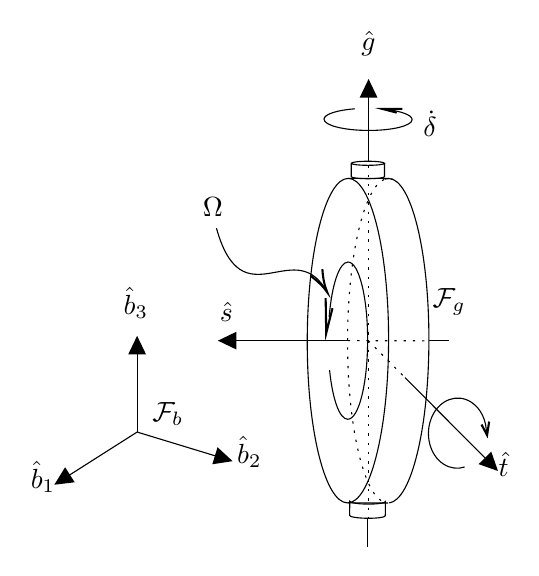
\begin{tikzpicture}[x=0.75pt,y=0.75pt,yscale=-1,xscale=1]
%uncomment if require: \path (0,336); %set diagram left start at 0, and has height of 336

%Shape: Ellipse [id:dp16305937027538286] 
\draw   (198.05,82.18) .. controls (187.23,82.16) and (178.38,117.14) .. (178.29,160.32) .. controls (178.2,203.5) and (186.9,238.52) .. (197.72,238.54) .. controls (208.54,238.57) and (217.39,203.58) .. (217.48,160.4) .. controls (217.57,117.23) and (208.87,82.21) .. (198.05,82.18) -- cycle ;
%Shape: Arc [id:dp5611693860078373] 
\draw  [draw opacity=0] (217.8,238.54) .. controls (228.32,237.19) and (236.81,202.75) .. (236.9,160.44) .. controls (236.99,117.27) and (228.29,82.25) .. (217.47,82.22) .. controls (216.86,82.22) and (216.26,82.33) .. (215.66,82.55) -- (217.31,160.4) -- cycle ; \draw   (217.8,238.54) .. controls (228.32,237.19) and (236.81,202.75) .. (236.9,160.44) .. controls (236.99,117.27) and (228.29,82.25) .. (217.47,82.22) .. controls (216.86,82.22) and (216.26,82.33) .. (215.66,82.55) ;
%Shape: Arc [id:dp4673444196641876] 
\draw  [draw opacity=0][dash pattern={on 0.84pt off 2.51pt}] (219.65,82.71) .. controls (218.94,82.39) and (218.21,82.23) .. (217.47,82.22) .. controls (206.65,82.2) and (197.8,117.19) .. (197.71,160.36) .. controls (197.63,201.84) and (205.65,235.79) .. (215.88,238.42) -- (217.31,160.4) -- cycle ; \draw  [dash pattern={on 0.84pt off 2.51pt}] (219.65,82.71) .. controls (218.94,82.39) and (218.21,82.23) .. (217.47,82.22) .. controls (206.65,82.2) and (197.8,117.19) .. (197.71,160.36) .. controls (197.63,201.84) and (205.65,235.79) .. (215.88,238.42) ;
%Straight Lines [id:da3790853736007833] 
\draw    (198.05,82.18) -- (217.64,82.22) ;
%Straight Lines [id:da49457185352382926] 
\draw    (197.72,238.54) -- (217.31,238.58) ;
%Straight Lines [id:da17676236612848806] 
\draw    (138.25,160.36) -- (197.88,160.36) ;
\draw [shift={(135.25,160.36)}, rotate = 0] [fill={rgb, 255:red, 0; green, 0; blue, 0 }  ][line width=0.08]  [draw opacity=0] (8.93,-4.29) -- (0,0) -- (8.93,4.29) -- cycle    ;
%Shape: Arc [id:dp4399957822164926] 
\draw  [draw opacity=0] (189.05,174.54) .. controls (190.43,188.43) and (193.82,198.23) .. (197.81,198.24) .. controls (203.05,198.25) and (207.33,181.3) .. (207.38,160.38) .. controls (207.42,139.46) and (203.21,122.5) .. (197.96,122.49) .. controls (193.72,122.48) and (190.1,133.59) .. (188.85,148.93) -- (197.88,160.36) -- cycle ; \draw   (189.05,174.54) .. controls (190.43,188.43) and (193.82,198.23) .. (197.81,198.24) .. controls (203.05,198.25) and (207.33,181.3) .. (207.38,160.38) .. controls (207.42,139.46) and (203.21,122.5) .. (197.96,122.49) .. controls (193.72,122.48) and (190.1,133.59) .. (188.85,148.93) ;
\draw  [line width=0.75]  (187.16,139.92) -- (187.42,156.81) -- (190.46,144.7) ;
%Straight Lines [id:da34755210780323087] 
\draw  [dash pattern={on 0.84pt off 2.51pt}]  (197.88,160.36) -- (237,160.45) ;
%Straight Lines [id:da33567491224781065] 
\draw    (237,160.45) -- (246.76,160.45) ;
%Straight Lines [id:da23155226852556665] 
\draw  [dash pattern={on 0.84pt off 2.51pt}]  (207.68,160.38) -- (207.68,245.94) ;
%Straight Lines [id:da35771586989491655] 
\draw    (207.29,259.9) -- (207.29,245.94) ;
%Straight Lines [id:da9106574700939476] 
\draw    (207.84,74.34) -- (207.84,37.31) ;
\draw [shift={(207.84,34.31)}, rotate = 450] [fill={rgb, 255:red, 0; green, 0; blue, 0 }  ][line width=0.08]  [draw opacity=0] (8.93,-4.29) -- (0,0) -- (8.93,4.29) -- cycle    ;
%Straight Lines [id:da20216065712708864] 
\draw  [dash pattern={on 0.84pt off 2.51pt}]  (207.68,75.89) -- (207.68,160.38) ;
%Shape: Arc [id:dp3776892833505412] 
\draw  [draw opacity=0] (215.57,48.87) .. controls (223.35,49.7) and (228.83,51.64) .. (228.82,53.87) .. controls (228.81,56.81) and (219.29,59.15) .. (207.57,59.09) .. controls (195.84,59.04) and (186.35,56.61) .. (186.36,53.67) .. controls (186.37,51.29) and (192.61,49.31) .. (201.21,48.67) -- (207.59,53.77) -- cycle ; \draw   (215.57,48.87) .. controls (223.35,49.7) and (228.83,51.64) .. (228.82,53.87) .. controls (228.81,56.81) and (219.29,59.15) .. (207.57,59.09) .. controls (195.84,59.04) and (186.35,56.61) .. (186.36,53.67) .. controls (186.37,51.29) and (192.61,49.31) .. (201.21,48.67) ;
\draw  [line width=0.75]  (224.09,48.67) -- (214.62,48.75) -- (221.4,50.5) ;

%Straight Lines [id:da42306237074586406] 
\draw    (225.4,178.18) -- (268.07,221.03) ;
\draw [shift={(270.19,223.16)}, rotate = 225.12] [fill={rgb, 255:red, 0; green, 0; blue, 0 }  ][line width=0.08]  [draw opacity=0] (8.93,-4.29) -- (0,0) -- (8.93,4.29) -- cycle    ;
%Straight Lines [id:da4976906999555484] 
\draw  [dash pattern={on 0.84pt off 2.51pt}]  (207.68,160.38) -- (225.4,178.18) ;
%Shape: Arc [id:dp8643023736796815] 
\draw  [draw opacity=0] (264.6,204.98) .. controls (264.66,198.91) and (262.02,193.04) .. (257.3,190) .. controls (250.53,185.63) and (242.05,188.78) .. (238.37,197.02) .. controls (234.69,205.26) and (237.2,215.49) .. (243.97,219.86) .. controls (247.2,221.94) and (250.82,222.32) .. (254.12,221.25) -- (250.64,204.93) -- cycle ; \draw   (264.6,204.98) .. controls (264.66,198.91) and (262.02,193.04) .. (257.3,190) .. controls (250.53,185.63) and (242.05,188.78) .. (238.37,197.02) .. controls (234.69,205.26) and (237.2,215.49) .. (243.97,219.86) .. controls (247.2,221.94) and (250.82,222.32) .. (254.12,221.25) ;
\draw  [line width=0.75]  (265.92,199.34) -- (264.94,205.9) -- (262.25,200.8) ;
%Curve Lines [id:da9723591382724126] 
\draw    (134.54,106.2) .. controls (147.07,150.75) and (171.19,110.03) .. (186.99,135.46) ;
\draw [shift={(187.95,137.1)}, rotate = 241.27] [color={rgb, 255:red, 0; green, 0; blue, 0 }  ][line width=0.75]    (10.93,-3.29) .. controls (6.95,-1.4) and (3.31,-0.3) .. (0,0) .. controls (3.31,0.3) and (6.95,1.4) .. (10.93,3.29)   ;
%Straight Lines [id:da23421207250028164] 
\draw    (96.32,161.05) -- (96.32,204.4) ;
\draw [shift={(96.32,158.05)}, rotate = 90] [fill={rgb, 255:red, 0; green, 0; blue, 0 }  ][line width=0.08]  [draw opacity=0] (8.93,-4.29) -- (0,0) -- (8.93,4.29) -- cycle    ;
%Straight Lines [id:da8003600910266351] 
\draw    (139.48,217.55) -- (96.32,204.4) ;
\draw [shift={(142.35,218.42)}, rotate = 196.94] [fill={rgb, 255:red, 0; green, 0; blue, 0 }  ][line width=0.08]  [draw opacity=0] (8.93,-4.29) -- (0,0) -- (8.93,4.29) -- cycle    ;
%Straight Lines [id:da5231524049233922] 
\draw    (58.94,228.17) -- (96.32,204.4) ;
\draw [shift={(56.41,229.78)}, rotate = 327.54] [fill={rgb, 255:red, 0; green, 0; blue, 0 }  ][line width=0.08]  [draw opacity=0] (8.93,-4.29) -- (0,0) -- (8.93,4.29) -- cycle    ;
%Shape: Can [id:dp3666821815276111] 
\draw   (215.5,74.91) -- (215.5,81.37) .. controls (215.5,81.91) and (211.92,82.35) .. (207.5,82.35) .. controls (203.08,82.35) and (199.5,81.91) .. (199.5,81.37) -- (199.5,74.91) .. controls (199.5,74.37) and (203.08,73.93) .. (207.5,73.93) .. controls (211.92,73.93) and (215.5,74.37) .. (215.5,74.91) .. controls (215.5,75.45) and (211.92,75.89) .. (207.5,75.89) .. controls (203.08,75.89) and (199.5,75.45) .. (199.5,74.91) ;
%Flowchart: Stored Data [id:dp10186943512192137] 
\draw   (198.71,244.56) -- (198.77,237.73) .. controls (198.76,238.45) and (202.6,239.07) .. (207.35,239.11) .. controls (212.09,239.15) and (215.95,238.6) .. (215.95,237.88) -- (215.89,244.72) .. controls (215.88,245.44) and (212.03,245.99) .. (207.29,245.94) .. controls (202.54,245.9) and (198.7,245.28) .. (198.71,244.56) -- cycle ;


% Text Node
\draw (88.61,133.55) node [anchor=north west][inner sep=0.75pt]    {$\hat{b}_{3}$};
% Text Node
\draw (143.3,205.28) node [anchor=north west][inner sep=0.75pt]    {$\hat{b}_{2}$};
% Text Node
\draw (43.86,217.35) node [anchor=north west][inner sep=0.75pt]    {$\hat{b}_{1}$};
% Text Node
\draw (102.38,188.87) node [anchor=north west][inner sep=0.75pt]    {$\mathcal{F}_{b}$};
% Text Node
\draw (237.43,134.17) node [anchor=north west][inner sep=0.75pt]    {$\mathcal{F}_{g}$};
% Text Node
\draw (203.11,9.84) node [anchor=north west][inner sep=0.75pt]    {$\hat{g}$};
% Text Node
\draw (134.93,140.57) node [anchor=north west][inner sep=0.75pt]    {$\hat{s}$};
% Text Node
\draw (269.17,213.02) node [anchor=north west][inner sep=0.75pt]    {$\hat{t}$};
% Text Node
\draw (232.94,48.46) node [anchor=north west][inner sep=0.75pt]    {$\dot{\delta }$};
% Text Node
\draw (126.68,90.2) node [anchor=north west][inner sep=0.75pt]    {$\Omega $};


\end{tikzpicture}

    \caption{Axis definition for generic Control Moment Gyroscope}
    \label{fig:tikCMG}
\end{figure}


Starting from initial gimbal angle $\displaystyle \delta_{0}$ spin and transverse axis as function of $\displaystyle \delta $ are evaluated in $\displaystyle \mathcal{F}_{b}$ as
\begin{equation}
\mathbf{R}( \delta ) =\cos \delta \ \mathbf{1} \ +\ ( 1-\cos \delta ) \ \hat{\mathbf{g}} \otimes \hat{\mathbf{g}} +\sin( \delta ) \ \hat{\mathbf{g}}^{\times }
\end{equation}
\begin{gather}
\hat{s}( t) =\ \mathbf{R}( \delta ) \ \hat{s}( t_{0})\\
\hat{t}( t) =\ \mathbf{R}( \delta ) \ \hat{t}( t_{0}) \notag
\end{gather}
\begin{equation}
\begin{pmatrix}
\hat{s}( t)\\
\hat{t}( t)
\end{pmatrix} =\begin{pmatrix}
\cos( \delta -\delta_{0}) & \sin( \delta -\delta_{0})\\
-\sin( \delta -\delta_{0}) & \cos( \delta -\delta_{0})
\end{pmatrix}\begin{pmatrix}
\hat{s}( t_{0})\\
\hat{t}( t_{0})
\end{pmatrix}
\end{equation}
Angular velocity vector gimbal frame $\displaystyle \mathcal{F}_{g}$ with respect to $\displaystyle \mathcal{F}_{b}$ is 
\begin{equation}
\omega _{\mathcal{F}_{g} /\mathcal{F}_{b}} =\dot{\delta}\hat{g}
\end{equation}
and angular velocity vector of reaction wheel frame $\displaystyle \mathcal{F}_{w}$ in $\displaystyle \mathcal{F}_{g}$ is represented as
\begin{equation}
\omega _{\mathcal{F}_{W} /\mathcal{F}_{g}} =\dot{\delta}\hat{g}
\end{equation}
Gimbal inertia matrix expressed in $\displaystyle \mathcal{F}_{G}$ as diagonal matrix with $\displaystyle J^{*}_{g}$ are gimbal frame inertia along superscript * represented as spin $\displaystyle \hat{s} \ $transverse $\displaystyle \hat{t}$ and $\displaystyle \hat{g}$ axis Subscript $G$ and $W$  $CMG$are used to identify gimbal, RW and CMG respectively.


\begin{gather}
J_{G} =\begin{pmatrix}
J^{s}_{G} & 0 & 0\\
0 & J^{t}_{G} & 0\\
0 & 0 & J^{g}_{G}
\end{pmatrix} \notag
\end{gather}
Flywheel inertia $\displaystyle J^s_{W}$ is much larger than gimbal inertia and is symmetric about $\displaystyle \hat{g}$ therefore $\displaystyle ^{\mathcal{F}_{W}} J_{W} =^{\mathcal{F} g} J_{s}$ thus reaction wheel inertia about spin axis are given by $\displaystyle J^{s}_{W}$ and $\displaystyle J^{t}_{W} =J^{g}_{W}$

\begin{equation}
J_{W} =\begin{pmatrix}
J^{s}_{W} & 0 & 0\\
0 & J^{t}_{W} & 0\\
0 & 0 & J^{t}_{W}
\end{pmatrix}
\end{equation}
Constant diagonal matrix $\displaystyle J_{g}$ and $\displaystyle J_{s}$ are expressed in $\displaystyle \mathcal{F}_{b}$ as
\begin{gather}
J_{G} =J^{s}_{G} \ \hat{s} \ \hat{s}^{T} +J^{t}_{G}\hat{t} \ \hat{t}^{T} +\ J^{g}_{G} \ \hat{g} \ \hat{g}^{T}\\
J_{W} =J^{s}_{W} \ \hat{s} \ \hat{s}^{T} +J^{t}_{W}\hat{t} \ \hat{t}^{T} +\ J^{g}_{W} \ \hat{g} \ \hat{g}^{T} \notag
\end{gather}
and tensor of inertia for CMG system is sum of gimbal and reaction wheel inertia and written in $\displaystyle \mathcal{F}_{b}$ \ as
\begin{equation}
J_{CMG} =J^{s}_{CMG} \ \hat{s} \ \hat{s}^{T} +J^{t}_{CMG}\hat{t} \ \hat{t}^{T} +\ J^{g}_{CMG} \ \hat{g} \ \hat{g}^{T}
\end{equation}
CMG as asymmetric moving masses, note that center of mass of reaction wheel does may have offset from gimbal axis inertia property of spacecraft change with gamble rotation and are function of $\displaystyle \delta ( t)$. Using axis angle rotation matrix $\displaystyle \mathbf{R}( \delta )$
\begin{equation}
J_{CMG}( \delta ) =J^{s}_{CMG} \ \mathbf{R}( \delta )\hat{s}_{0} \ \hat{s}^{T}_{0}\mathbf{R}( \delta )^{T} +J^{t}_{CMG}\mathbf{R}( \delta )\hat{t} \ \hat{t}^{T}\mathbf{R}( \delta )^{T} +\ J^{g}_{CMG} \ \hat{g} \ \hat{g}^{T}
\end{equation}
We can see that $\displaystyle J_{CMG}$ is not constant and in order to realize angular momentum of CMG in body frame we need to evaluate derivative of CMG inertia tensor

\begin{equation}
\begin{aligned}
\dot{J}_{CMG} & =J^{s}_{CMG} \ \left[\dot{\hat{s}} \ \hat{s} +\hat{s} \ \dot{\hat{s}}\right] +J^{t}_{CMG}\left[\dot{\hat{t}} \ \hat{t} +\hat{t} \ \dot{\hat{t}}\right]\\
 & =\dot{\delta}\left( J^{s}_{CMG} -J^{t}_{CMG}\right)[\hat{t} \ \hat{s} +\hat{s} \ \hat{t}]
\end{aligned}
\label{eqn:Jcmg_dot}
\end{equation}

From \autoref{eqn:Jcmg_dot} we can say that derivative of CMG inertia tensor is function of gimbal velocity and difference in moment of inertia about spin and transverse axis. Since these are very small compared and $\displaystyle \dot{J}_{CMG}$ is also very low compared to spacecraft inertia.

We have velocity $\displaystyle \omega $ of spacecraft body frame $\displaystyle \mathcal{F}_{b}$ measured in inertial frame $\displaystyle \mathcal{F}_{i}$ now angular velocity $\displaystyle \omega _{G}$ and $\displaystyle \omega_{w}$of gimbal and flywheel are represented in terms  gimbal angular velocity $\displaystyle \Omega_{G}$ and RW angular velocity $\displaystyle \Omega _{W}$ is


\begin{equation}
\begin{aligned}
\omega _{G} & =\omega +\Omega _{G} =\omega +\dot{\delta}\hat{g}\\
\omega _{W} & =\omega +\Omega _{W} =\omega +\dot{\delta}\hat{g} +\Omega \hat{s}
\end{aligned}
\label{eqn:omega_inG}
\end{equation}

From \autoref{eqn:Jcmg_dot} and \autoref{eqn:omega_inG} Gimbal angular momentum $\displaystyle\mathcal{H}_{G}$, RW angular momentum $\displaystyle \mathcal{H}_{W}$, \ and CMG angular momentum $\displaystyle \mathcal{H}_{CMG}$ \ are evaluated as


\begin{equation}
\begin{aligned}
\mathcal{H}_{G} & =J_{G} \cdotp \omega _{G}\\
 & =\omega +\dot{\delta}\hat{g}\\
 & =J_{G} \cdotp \omega +J^{g}_{G} \ \dot{\delta \ }\hat{g}
\end{aligned}
\end{equation}
RW Momentum,
\begin{equation}
\begin{aligned}
\mathcal{H}_{W} & =J_{W} \cdotp \omega _{W}\\
 & =\omega +\dot{\delta}\hat{g} +\Omega \hat{s}\\
 & =J_{W} \cdotp \omega +J^{g}_{W} \ \dot{\delta} \ \hat{g} +J^s_{W} \ \Omega \hat{s}
\end{aligned}
\end{equation}
CMG Momentum is sum of RW abd Gimbal momentum as,
\begin{equation}
\begin{aligned}
\mathcal{H}_{CMG} & =\mathcal{H}_{G} +\mathcal{H}_{W}\\
 & =( J_{G} +J_{W}) \cdotp \omega +\ \left( J^{g}_{G} +J^{g}_{W}\right)\dot{\delta} \ \hat{g} +J_{W} \ \Omega \ \hat{s}\\
 & =J_{CMG}( \delta ) \cdotp \omega +\ J^{g}_{CMG} \ \dot{\delta} \ \hat{g} +J^s_{W} \ \Omega \ \hat{s}
\end{aligned}\\
\label{eqn_Hcmg}
\end{equation}
From \autoref{eqn_Hcmg} we can say that CMG angular momentum is function of body, gimbal, RW angular velocity and gimbal angle $\delta$

\section{Spacecraft Attitude Dynamics}
Rigid body having angular momentum $\displaystyle \mathcal{H}$ with respect to center of mass and applied torque $\displaystyle \mathbf{\tau }$, From newton Euler rigid body dynamics we know that rate of change of angular momentum of body is equal to torque applied to it. Time rate of change of angular momentum in body frame is
\begin{gather}
\frac{d\mathcal{H}}{dt} =\mathbf{\tau }\\
\dot{\mathcal{H}} =\mathbf{\tau } \notag
\end{gather}
Using transport theorem derivative of angular momentum expressed in $\displaystyle \mathcal{F}_{I}$ gives us Newton Euler equation for attitude dynamics.
\begin{equation}
\dot{\mathcal{H}} +\omega \times \mathcal{H} =\tau 
\label{eqn:NewtonEulerB}
\end{equation}

\noindent Assuming the hypothesis of rigid body and neglecting all elastic properties of spacecraft in free falling orbit we can expand the torque $\displaystyle \tau $ as combination of disturbance torque $\displaystyle \tau _{d}$ external environmental torque $\displaystyle \tau _{e}$ and control torque $\displaystyle \mathbf{u}$ thus \autoref{eqn:NewtonEulerB} becomes
\begin{equation}
\dot{\mathcal{H}} +\omega \times \mathcal{H} =\tau _{d} +\tau _{e} +\mathbf{u}
\label{eqn:NewtonEulerI}
\end{equation}
Environmental torques $\displaystyle \tau _{e}$ are the major source of external disturbances that influence dynamics of spacecraft. Gravity gradient torques acting on spacecraft due to variation in gravitational pull acting on distributed mass, they provide small but have significant contribution over the period of time. Due to center of pressure is not coincident with center of mass presence of very small air density at Low Earth Orbit, variation in aerodynamic forces distribution causes couple around center of mass. Magnetic materials and current flowing through electrical systems interacts with earths magnetic field causing contributes to external torque. Solar radiation pressure on spacecraft surface exposed to sun produces torque generally significant amount at Geostationary Orbits. These torques $\displaystyle \tau _{e}$ are known and can be modeled. On the other hand those which are not modeled are disturbance torques $\displaystyle \tau _{d}$ these are due to elastic modes, thruster misalignment, uncertainty in center of gravity and rotating parts.

\noindent The demand control torque $\displaystyle \mathbf{u}$ is provided by actuators such as thrusters, momentum devices, magnetotorquer in order to reorient the spacecraft in desired states or to maintain its attitude based on mission requirements. Following section discuss the modeling of momentum deceives to produce $\displaystyle \mathbf{u}$. Bearing in mind that momentum exchange devices operate on the principle of distributing angular momentum among parts of system keeping total angular momentum conserved as a consequence $\displaystyle \mathbf{u}$ is zero as long as any external saturation system is not present. Other torques $\displaystyle \tau _{e}$ and $\displaystyle \tau _{d}$ are disregarded for preliminary modeling. Accordingly equation becomes
\begin{equation}
\dot{\mathcal{H}} +\omega \times \mathcal{H} = 0
\label{eqn:TorqueFreeEOM}
\end{equation}
For the spacecraft equipped with CMG $\displaystyle \mathcal{H}$ is sum of angular momentum of spacecraft platform $\displaystyle \mathcal{H}_{P}$ and CMG $\displaystyle \mathcal{H}_{CMG}$. Whereas Inertia tensor of platform is
\begin{equation}
J_{P} =J_{P,0} +m\sum ^{n}_{k=1}( ||\vec{\mathbf{d}}_{k} ||\ \vec{\mathbf{1}} -\vec{\mathbf{d}}_{k}\vec{\mathbf{d}}_{k})
\end{equation}
Here, $\displaystyle J_{P,0}$ is inertia of platform without CMG and $\displaystyle m$ is mass of $\displaystyle k^{th}$ CMG whose center of mass is at distance $\displaystyle \vec{\mathbf{d}}_{k}$ from center of mass of entire system. The angular momentum of platform is
\begin{equation}
\mathcal{H}_{P} =J_{P} \cdotp \omega 
\end{equation}

Total system angular momentum of spacecraft equipped \ with $\displaystyle n$ number of SGCMGs is 
\begin{tcolorbox}
\begin{equation}
\begin{aligned}
\mathcal{H} & =\mathcal{H}_{P} +\sum ^{n}_{k=1}\mathcal{H}^{k}_{CMG}\\
 & =J_{P} \cdotp \omega +\sum ^{n}_{k=1}\left( J^{k}_{CMG}( \delta_{k}) \cdotp \omega +\ J^{g}_{CMG} \ \dot{\delta}_{k} \ \hat{g}_{k} +J^{s}_{W} \ \Omega _{k} \ \hat{s}_{k}\right)\\
 & =\left[ J_{P} +\sum ^{n}_{k=1} J^{k}_{CMG}( \delta_{k})\right] \cdotp \omega +\ J^{g}_{CMG} \ \sum ^{n}_{k=1}\dot{\delta}_{k} \ \hat{g}_{k} +J^{s}_{W}\sum ^{n}_{k=1} \ \Omega _{k} \ \hat{s}_{k}
\end{aligned}\\
\label{eqn:H_Total}
\end{equation}
\end{tcolorbox}

Time derivative of \autoref{eqn:H_Total} in platform frame $\mathcal{H}_P$ is expressed as

\begin{equation}
\begin{aligned}
\frac{d\mathcal{H}}{dt} & =\left[ J_{P} +\sum ^{n}_{k=1} J^{k}_{CMG}( \delta_{k})\right] \cdotp \dot{\omega } +\\
 & +\sum ^{n}_{k=1}\dot{J}^{k}_{CMG}( \delta_{k}) \cdotp \omega +\\
 & +\ J^{g}_{CMG}\sum ^{n}_{k=1} \ \ddot{\delta}_{k} \ \hat{g}_{k} +J^{s}_{W}\sum ^{n}_{k=1} \ \dot{\Omega }_{k} \ \hat{s}_{k} +\ J^{s}_{W} \ \sum ^{n}_{k=1} \Omega _{k}\dot{\delta}_{k} \ \hat{t}_{k}
\end{aligned}
\end{equation}Substituting inertia derivative from \autoref{eqn:Jcmg_dot} we have
\begin{equation}
\begin{aligned}
\dot{\mathcal{H}} & =\left[ J_{P} +\sum ^{n}_{k=1} J^{k}_{CMG}( \delta_{k})\right] \cdotp \dot{\omega } +\\
 & +\dot{\delta}\left( J^{s}_{CMG} -J^{t}_{CMG}\right)\sum ^{n}_{k=1}(\hat{t}_{k} \ \hat{s}_{k} +\hat{s}_{k} \ \hat{t}_{k}) \cdotp \omega +\\
 & +\ J^{g}_{CMG} \ \sum ^{n}_{k=1}\ddot{\delta}_{k} \ \hat{g}_{k} +J^{s}_{W}\sum ^{n}_{k=1} \ \dot{\Omega }_{k} \ \hat{s}_{k} +\ J^{s}_{W} \ \sum ^{n}_{k=1} \Omega _{k}\dot{\delta}_{k} \ \hat{t}_{k}
\end{aligned}
\label{eqn:TorqueFreeEOM_H}
\end{equation}
Cross multiplying \autoref{eqn:H_Total} by body angular velocity $\omega$ we get gyroscopic part of Euler attitude equation
\begin{equation}
\begin{aligned}
\omega \times \mathcal{H} & =\omega \times \left[ J_{P} +\sum ^{n}_{k=1} J^{k}_{CMG}( \delta_{k})\right] \cdotp \omega \\
 & +\ J^{g}_{CMG} \ \omega \times \sum ^{n}_{k=1}\dot{\delta}_{k} \ \hat{g}_{k}\\
 & +\ J^{s}_{W} \omega \times \sum ^{n}_{k=1} \ \Omega _{k} \ \hat{s}_{k}
\end{aligned}
\label{eqn:TorqueFreeEOM_xH}
\end{equation}
Substituting \autoref{eqn:TorqueFreeEOM_xH} and \autoref{eqn:TorqueFreeEOM_xH} in to \autoref{eqn:TorqueFreeEOM} we have Generalized attitude dynamics of a rigid satellite equipped with a cluster of $\displaystyle n$ identical single gimbal VSCMGs
%///////////////VSCMG EOM/////////////////////


\begin{tcolorbox}
\begin{equation}
\begin{aligned}
\dot{\mathcal{H}} +\omega \times \mathcal{H} & =
\left[ J_{P} +\sum ^{n}_{k=1} J^{k}_{CMG}( \delta_{k})\right] \cdotp \dot{\omega }+\omega \times \left[ J_{P} +\sum ^{n}_{k=1} J^{k}_{CMG}( \delta_{k})\right] \cdotp \omega \\
 & +\ \dot{\delta}\left( J^{s}_{CMG} -J^{t}_{CMG}\right)\sum ^{n}_{k=1}(\hat{t}_{k} \ \hat{s}_{k} +\hat{s}_{k} \ \hat{t}_{k}) \cdotp \omega \\
 & +\ J^{s}_{W}\sum ^{n}_{k=1} \ \dot{\Omega }_{k} \ \hat{s}_{k} +\ J^{s}_{W} \ \sum ^{n}_{k=1} \Omega _{k}\dot{\delta}_{k} \ \hat{t}_{k} +\ J^{s}_{W} \omega \times \sum ^{n}_{k=1} \ \Omega _{k} \ \hat{s}_{k}\\
 & +J^{g}_{CMG} \ \sum ^{n}_{k=1}\ddot{\delta}_{k} \ \hat{g}_{k} +J^{g}_{CMG} \ \omega \times \sum ^{n}_{k=1}\dot{\delta}_{k} \ \hat{g}_{k}
\end{aligned}
\label{eqn:EOM_FULL}
\end{equation}
\end{tcolorbox}

%//////////////////END EOM/////////////////////
Dynamical equation \autoref{eqn:EOM_FULL} is composition of contribution effects due to spacecraft angular velocity, gyroscopic effects the angular momentum of the entire system, variation of moment of inertia flywheel and gimbal velocities explained in \autoref{tab:vscmg_eom_explain} as reasoning \ of each terms contribution in entire system dynamics.A generalized dynamics for a satellite equipped with generic number of momentum exchange devices. We can see that this equation of motion comprises dynamics of reaction wheel, CMG and VSCMG 
\begin{table}[!ht]
\centering
\begin{tabular}{p{0.30\textwidth}||p{0.7\textwidth}}
\toprule
\begin{center} Contribution rationale  \end{center}& \begin{center}
     Term
 \end{center} \\
\midrule
Variation of satellite angular velocity & 
\begin{equation*}
\left[ J_{P} +\sum ^{n}_{k=1} J^{k}_{CMG}( \delta_{k})\right] \cdotp \dot{\omega }
\vspace{-1em}\end{equation*} \\
\hline 
 Gyroscopic effects due to angular momentum of entire system & 
\begin{equation*}
\omega \times \left[ J_{P} +\sum ^{n}_{k=1} J^{k}_{CMG}( \delta_{k})\right] \cdotp \omega 
\vspace{-1em}\end{equation*} \\
\hline 
 variation of the tensor of inertia & 
\begin{equation*}
\dot{\delta}\left( J^{s}_{CMG} -J^{t}_{CMG}\right)\sum ^{n}_{k=1}(\hat{t}_{k} \ \hat{s}_{k} +\hat{s}_{k} \ \hat{t}_{k}) \cdotp \omega 
\vspace{-1em}\end{equation*} \\
\hline 
variation reaction wheel velocities & 
\begin{equation*}
\ J^{s}_{W}\sum ^{n}_{k=1} \ \dot{\Omega }_{k} \ \hat{s}_{k} +\ J^{s}_{W} \ \sum ^{n}_{k=1} \Omega _{k}\dot{\delta}_{k} \ \hat{t}_{k} +\ J^{s}_{W} \omega \times \sum ^{n}_{k=1} \ \Omega _{k} \ \hat{s}
\vspace{-1em}\end{equation*} \\
\hline 
 variation of gimbals velocities & 
\begin{equation*}
J^{g}_{CMG} \ \sum ^{n}_{k=1}\ddot{\delta}_{k} \ \hat{g}_{k} +J^{g}_{CMG} \ \omega \times \sum ^{n}_{k=1}\dot{\delta}_{k} \ \hat{g}_{k}
\vspace{-1em}\end{equation*} \\
\bottomrule
\end{tabular}
    \caption{Explanation of individual terms in generalize equation of motion for satellite with generic number of VSCMG}
    \label{tab:vscmg_eom_explain}
\end{table}

\subsection{Reaction Wheel (RW)}
If we freeze the gimbal, i.e. $\displaystyle \dot{\delta} =0$ in \autoref{eqn:EOM_FULL}, resultant equation is satellite with reaction wheels simplified as
\begin{equation}
\dot{\mathcal{H}} +\omega \times \mathcal{H} =J \cdotp \dot{\omega } +\omega \times J \cdotp \omega +\ J^{s}_{W}\sum ^{n}_{k=1} \ \dot{\Omega }_{k} \ \hat{s}_{k} +\ J^{s}_{W} \omega \times \sum ^{n}_{k=1} \ \Omega _{k} \ \hat{s}_{k} =0
\end{equation}
here $\displaystyle J=J_{P} +\sum ^{n}_{k=1} J^{k}_{CMG}$ and derivative of $\displaystyle \dot{J}$ is zero. For regulation maneuver which conveys maintain fixed attitude counteracting the external disturbance making body rate $\displaystyle \omega =0$ becomes.
\begin{equation}
J^{s}_{W}\sum ^{n}_{k=1} \ \dot{\Omega }_{k} \ \hat{s}_{k} =\tau _{d}
\end{equation}
Three reaction wheels with their spin axis mutually perpendicular are sufficient to counteract disturbance in any axis as long as saturation (maximum limit of angular momentum) does not occurs. Output torque is torque is proportional to rate of change of RW angular velocity and moment of inertia.

\subsection{Control Moment Gyroscope (CMG)}
Keeping angular velocity of RW \ $\displaystyle \Omega $ constant in \autoref{eqn:EOM_FULL} we get e attitude equation of a satellite equipped with control moment gyros as 
\begin{equation}
\begin{aligned}
\dot{\mathcal{H}} +\omega \times \mathcal{H} & =\left[ J_{P} +\sum ^{n}_{k=1} J^{k}_{CMG}( \delta_{k})\right] \cdotp \dot{\omega } +\omega \times \left[ J_{P} +\sum ^{n}_{k=1} J^{k}_{CMG}( \delta_{k})\right] \cdotp \omega \\
 & +\ \dot{\delta}\left( J^{s}_{CMG} -J^{t}_{CMG}\right)\sum ^{n}_{k=1}(\hat{t}_{k} \ \hat{s}_{k} +\hat{s}_{k} \ \hat{t}_{k}) \cdotp \omega \\
 & +\ J^{s}_{W} \ \sum ^{n}_{k=1} \Omega _{k}\dot{\delta}_{k} \ \hat{t}_{k} +\ J^{s}_{W} \omega \times \sum ^{n}_{k=1} \ \Omega _{k} \ \hat{s}_{k}\\
 & +J^{g}_{CMG} \ \sum ^{n}_{k=1}\ddot{\delta}_{k} \ \hat{g}_{k} +J^{g}_{CMG} \ \omega \times \sum ^{n}_{k=1}\dot{\delta}_{k} \ \hat{g}_{k}
\end{aligned}
\end{equation}


For regulation maneuver disturbance torque can be counteracted as
\begin{equation}
J^{s}_{W} \ \sum ^{n}_{k=1} \Omega _{k}\dot{\delta}_{k} \ \hat{t}_{k} +J^{g}_{CMG} \ \sum ^{n}_{k=1}\ddot{\delta}_{k} \ \hat{g}_{k} =\tau _{d}
\label{eqb:cmg_tau_d}
\end{equation}
Torque produced through CMG is sum of gyroscopic couple due to variation in RW axis variation and acceleration of gimbal frame. Since moment of inertia of CMG and acceleration along gimbal axis is very small \autoref{eqb:cmg_tau_d} is simplified as
\begin{equation}
J^{s}_{W} \ \sum ^{n}_{k=1} \Omega _{k}\dot{\delta}_{k} \ \hat{t}_{k} =\tau _{d}
\label{eqn:cmg_tau}
\end{equation}
\autoref{eqn:cmg_tau} is torque amplification due to gyroscopic effects of RW in body frame which is larger compared to RW. CMG torques are along transverse axis $\displaystyle \hat{t}$ moving in $\displaystyle \mathcal{F}_{b}$ and cannot produce orthogonal torque known as singularity.
\begin{equation}
\begin{aligned}
\dot{\mathcal{H}} +\omega \times \mathcal{H} & =\left[ J_{P} +\sum ^{n}_{k=1} J^{k}_{CMG}( \delta_{k})\right] \cdotp \dot{\omega } +\omega \times \left[ J_{P} +\sum ^{n}_{k=1} J^{k}_{CMG}( \delta_{k})\right] \cdotp \omega \\
 & +\ \dot{\delta}\left( J^{s}_{CMG} -J^{t}_{CMG}\right)\sum ^{n}_{k=1}(\hat{t}_{k} \ \hat{s}_{k} +\hat{s}_{k} \ \hat{t}_{k}) \cdotp \omega \\
 & +\ J^{s}_{W} \ \sum ^{n}_{k=1} \Omega _{k}\dot{\delta}_{k} \ \hat{t}_{k} +\ J^{s}_{W} \omega \times \sum ^{n}_{k=1} \ \Omega _{k} \ \hat{s}_{k}\\
 & +J^{g}_{CMG} \ \sum ^{n}_{k=1}\ddot{\delta}_{k} \ \hat{g}_{k} +J^{g}_{CMG} \ \omega \times \sum ^{n}_{k=1}\dot{\delta}_{k} \ \hat{g}_{k}
\end{aligned}
\end{equation}
For regulation maneuver torque is evaluated as
\begin{equation}
J^{s}_{W} \ \sum ^{n}_{k=1} \Omega _{k}\dot{\delta}_{k} \ \hat{t}_{k} +J^{g}_{CMG} \ \sum ^{n}_{k=1}\ddot{\delta}_{k} \ \hat{g}_{k} =\tau _{d}
\end{equation}
Simplified for small gimbal acceleration, regulation maneuver torque
\begin{equation}
J^{s}_{W} \ \sum ^{n}_{k=1} \Omega _{k}\dot{\delta}_{k} \ \hat{t}_{k} =\tau _{d}
\end{equation}
\subsection{Variable Speed Control Moment Gyroscope (VSCMG)}

Taking advantage from both reaction wheel and CMG for regulation maneuver to neutralize external disturbance $\displaystyle \tau _{d}$ we have
\begin{equation}
\ J^{s}_{W}\sum ^{n}_{k=1} \ \dot{\Omega }_{k} \ \hat{s}_{k} +J^{s}_{W} \ \sum ^{n}_{k=1} \Omega _{k}\dot{\delta}_{k} \ \hat{t}_{k} +J^{g}_{CMG} \ \sum ^{n}_{k=1}\ddot{\delta}_{k} \ \hat{g}_{k} =\tau _{d}
\end{equation}
is combination of RW and torque amplification due to CMG. Trivial presence in CMG can be escaped with RW and high torques are generated with gyroscopic forces. This thesis focuses on VSCMG with pyramid cluster. In order to simplify numerical computation direction vectors can be arranged in matrix form. For n-VSCMG, Unit direction vectors of Gimbal, Spin and Transverse axis axis are evaluated based on their initial orientation

\begin{gather}
\mathcal{G}_{g} =[\hat{g}_{1} \cdots \ \hat{g}_{n}]_{3\times n} =\mathcal{G}_{g0} \notag\\
\mathcal{G}_{s} \ =\ [\hat{s}_{1} \cdots \ \hat{s}_{n}]_{3\times n} =\mathcal{G}_{s0}\cos \delta +\mathcal{G}_{t0}\sin \delta  \notag\\
\mathcal{G}_{t} \ =[\hat{t}_{1} \cdots \ \hat{t}_{n}]_{3\times n} =\mathcal{- G_{s0}\sin \delta +G}_{t0}\cos \delta 
\end{gather}

This thesis is focused on pyramid cluster of four VSCMG units. Single Gimbal Control Moment Gyroscope basis vectors, initially orientation of each CMG spin and gimbal axis is shown in \autoref{fig:VSCMGPyramid} with gimbal axis skewed by angle $\beta$.


\tikzset{every picture/.style={line width=0.75pt}} %set default line width to 0.75pt
\begin{figure}[h]
\centering


\tikzset{every picture/.style={line width=0.75pt}} %set default line width to 0.75pt        

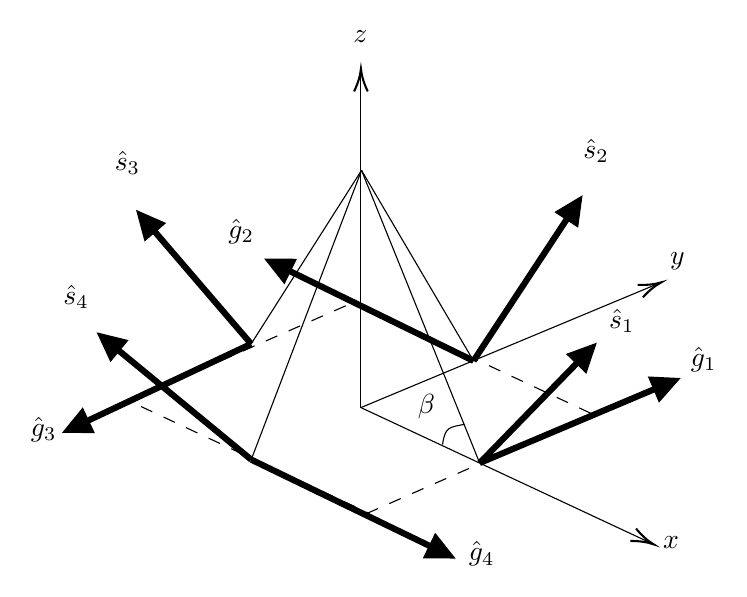
\begin{tikzpicture}[x=0.75pt,y=0.75pt,yscale=-1,xscale=1]
%uncomment if require: \path (0,260); %set diagram left start at 0, and has height of 260

%Shape: Rectangle [id:dp017783013341910126] 
\draw  [dash pattern={on 4.5pt off 4.5pt}] (307.47,113.95) -- (422.51,167.82) -- (314.44,215.41) -- (199.4,161.55) -- cycle ;
%Straight Lines [id:da44988304357834097] 
\draw    (310.95,164.68) -- (450.2,229.75) ;
\draw [shift={(452.01,230.59)}, rotate = 205.05] [color={rgb, 255:red, 0; green, 0; blue, 0 }  ][line width=0.75]    (10.93,-3.29) .. controls (6.95,-1.4) and (3.31,-0.3) .. (0,0) .. controls (3.31,0.3) and (6.95,1.4) .. (10.93,3.29)   ;
%Straight Lines [id:da3169132363517273] 
\draw    (310.95,164.68) -- (310.95,3.43) ;
\draw [shift={(310.95,1.43)}, rotate = 450] [color={rgb, 255:red, 0; green, 0; blue, 0 }  ][line width=0.75]    (10.93,-3.29) .. controls (6.95,-1.4) and (3.31,-0.3) .. (0,0) .. controls (3.31,0.3) and (6.95,1.4) .. (10.93,3.29)   ;
%Straight Lines [id:da03800207830963842] 
\draw [line width=2.25]    (368.16,191.38) -- (460.41,152.4) ;
\draw [shift={(465.02,150.45)}, rotate = 517.0899999999999] [fill={rgb, 255:red, 0; green, 0; blue, 0 }  ][line width=0.08]  [draw opacity=0] (14.29,-6.86) -- (0,0) -- (14.29,6.86) -- cycle    ;
%Straight Lines [id:da7176914327617441] 
\draw    (310.95,164.68) -- (453.78,105.11) ;
\draw [shift={(455.63,104.35)}, rotate = 517.36] [color={rgb, 255:red, 0; green, 0; blue, 0 }  ][line width=0.75]    (10.93,-3.29) .. controls (6.95,-1.4) and (3.31,-0.3) .. (0,0) .. controls (3.31,0.3) and (6.95,1.4) .. (10.93,3.29)   ;
%Straight Lines [id:da7179733571465603] 
\draw [line width=2.25]    (171.44,174.72) -- (258.05,134.01) ;
\draw [shift={(166.92,176.85)}, rotate = 334.82] [fill={rgb, 255:red, 0; green, 0; blue, 0 }  ][line width=0.08]  [draw opacity=0] (14.29,-6.86) -- (0,0) -- (14.29,6.86) -- cycle    ;
%Straight Lines [id:da8667824746636326] 
\draw [line width=2.25]    (258.1,189.75) -- (352.1,235.22) ;
\draw [shift={(356.6,237.4)}, rotate = 205.81] [fill={rgb, 255:red, 0; green, 0; blue, 0 }  ][line width=0.08]  [draw opacity=0] (14.29,-6.86) -- (0,0) -- (14.29,6.86) -- cycle    ;
%Straight Lines [id:da9218968130041245] 
\draw [line width=2.25]    (365.19,142.16) -- (268.78,95.07) ;
\draw [shift={(264.29,92.88)}, rotate = 386.03] [fill={rgb, 255:red, 0; green, 0; blue, 0 }  ][line width=0.08]  [draw opacity=0] (14.29,-6.86) -- (0,0) -- (14.29,6.86) -- cycle    ;
%Straight Lines [id:da6650223825146806] 
\draw [line width=2.25]    (368.16,191.38) -- (421.11,136.98) ;
\draw [shift={(424.6,133.4)}, rotate = 494.23] [fill={rgb, 255:red, 0; green, 0; blue, 0 }  ][line width=0.08]  [draw opacity=0] (14.29,-6.86) -- (0,0) -- (14.29,6.86) -- cycle    ;
%Straight Lines [id:da37227200254977566] 
\draw [line width=2.25]    (365.19,142.16) -- (414.99,66.52) ;
\draw [shift={(417.74,62.34)}, rotate = 483.36] [fill={rgb, 255:red, 0; green, 0; blue, 0 }  ][line width=0.08]  [draw opacity=0] (14.29,-6.86) -- (0,0) -- (14.29,6.86) -- cycle    ;
%Straight Lines [id:da8487690207159158] 
\draw [line width=2.25]    (258.05,134.01) -- (205.86,73.19) ;
\draw [shift={(202.6,69.4)}, rotate = 409.36] [fill={rgb, 255:red, 0; green, 0; blue, 0 }  ][line width=0.08]  [draw opacity=0] (14.29,-6.86) -- (0,0) -- (14.29,6.86) -- cycle    ;
%Straight Lines [id:da10313815978305096] 
\draw [line width=2.25]    (258.1,189.75) -- (187.46,131.58) ;
\draw [shift={(183.6,128.4)}, rotate = 399.47] [fill={rgb, 255:red, 0; green, 0; blue, 0 }  ][line width=0.08]  [draw opacity=0] (14.29,-6.86) -- (0,0) -- (14.29,6.86) -- cycle    ;
%Straight Lines [id:da577231942329048] 
\draw    (311.24,50.38) -- (368.16,191.38) ;
%Straight Lines [id:da021184935151887796] 
\draw    (311.24,50.38) -- (258.1,189.75) ;
%Straight Lines [id:da9892209684505493] 
\draw    (311.24,50.38) -- (258.05,134.01) ;
%Straight Lines [id:da6195700121447263] 
\draw    (311.24,50.38) -- (365.19,142.16) ;
%Curve Lines [id:da0914926090159498] 
\draw    (350.28,182.46) .. controls (351.53,173.5) and (353.86,174.28) .. (360.87,172.72) ;

% Text Node
\draw (468.7,134.14) node [anchor=north west][inner sep=0.75pt]    {$\hat{g}_{1}$};
% Text Node
\draw (245.81,72.81) node [anchor=north west][inner sep=0.75pt]    {$\hat{g}_{2}$};
% Text Node
\draw (361.74,228.05) node [anchor=north west][inner sep=0.75pt]    {$\hat{g}_{4}$};
% Text Node
\draw (150.66,167.97) node [anchor=north west][inner sep=0.75pt]    {$\hat{g}_{3}$};
% Text Node
\draw (429.3,115.9) node [anchor=north west][inner sep=0.75pt]    {$\hat{s}_{1}$};
% Text Node
\draw (416.84,34.11) node [anchor=north west][inner sep=0.75pt]    {$\hat{s}_{2}$};
% Text Node
\draw (191.08,40.08) node [anchor=north west][inner sep=0.75pt]    {$\hat{s}_{3}$};
% Text Node
\draw (166.37,104.54) node [anchor=north west][inner sep=0.75pt]    {$\hat{s}_{4}$};
% Text Node
\draw (337.16,156.94) node [anchor=north west][inner sep=0.75pt]    {$\beta $};
% Text Node
\draw (455.25,225.33) node [anchor=north west][inner sep=0.75pt]    {$x$};
% Text Node
\draw (458.67,88.63) node [anchor=north west][inner sep=0.75pt]    {$y$};
% Text Node
\draw (306,-18.09) node [anchor=north west][inner sep=0.75pt]    {$z$};


\end{tikzpicture}

\caption{VSCMG Pyramid Cluster initial orientation}
\label{fig:VSCMGPyramid}
\end{figure}

Evaluation of commutative gimbal, spin and transverse axis in represented as $\mathcal{G}_g$,$\mathcal{G}_s$ and $\mathcal{G}_t$ respectively about body frame $\mathcal{G}_b$ with basis vector ${b_1,b_2,b_3}$ alinged with ${x,y,x}$. Gimbale axis of all CMGs are oriented by Skew angle $\beta$ is given as
\begin{equation}
\mathcal{G}_g = 
\begin{pmatrix}
 -\sin{}\beta &      0 & \sin{\beta} &       0 \\
       0 & \sin{\beta} &      0 & -\sin{\beta} \\
  \cos{\beta} & \cos{\beta} & \cos{\beta} &  \cos{\beta}
\end{pmatrix}
\end{equation}
\begin{equation}
\mathcal{G}_s =
\begin{pmatrix}
\cos{\beta} \cos{\delta_1} & -\sin{\delta_2} & -\cos{\beta} \cos{\delta_3} &  \sin{\delta_4} \\
-\sin{\delta_1} & -\cos{\beta} \cos{\delta_2} &  \sin{\delta_3} &  \cos{\beta} \cos{\delta_4} \\
\sin{\beta} \cos{\delta_1} &  \sin{\beta} \cos{\delta_2} &  \sin{\beta} \cos{\delta_3} &  \sin{\beta} \cos{\delta_4} 
\end{pmatrix}
\end{equation}
\begin{equation}
\mathcal{G}_t =
\begin{pmatrix}
\cos{\beta} \sin{\delta_1} &         \cos{\delta_2} & -\cos{\beta} \sin{\delta_3} &       -\cos{\delta_4} \\
       \cos{\delta_1} & -\cos{\beta} \sin{\delta_2} &        -\cos{\delta_3} & \cos{\beta} \sin{\delta_4} \\
\sin{\beta} \sin{\delta_1} &  \sin{\beta} \sin{\delta_2} &  \sin{\beta} \sin{\delta_3} & \sin{\beta} \sin{\delta_4}
\end{pmatrix}
\end{equation}

\autoref{eqn:EOM_FULL} can be written in the form of matrix for as 
\begin{tcolorbox}
\begin{equation}
\begin{aligned}
\dot{\mathcal{H}} +\omega \times \mathcal{H} & =J\dot{\omega } +\omega ^{\times }\left( J\omega +\mathcal{G}_{t} J^{g}_{CMG}\dot{\delta } +\mathcal{G}_{s} J^{s}_{W} \Omega \right)\\
 & +\mathcal{G}_{t}[\dot{\delta }]^{d}\left( J^{s}_{CMG} -J^{t}_{CMG}\right)\mathcal{G}^{T}_{s} +\mathcal{G}_{s}[\dot{\delta }]^{d}\left( J^{s}_{CMG} -J^{t}_{CMG}\right)\mathcal{G}^{T}_{t}\\
 & +\mathcal{G}_{t} J^{s}_{W}[ \Omega ]^{d}\dot{\delta } +\mathcal{G}_{s} J^{s}_{W}\dot{\Omega } +\mathcal{G} J^{g}_{CMG}\ddot{\delta }\\
 & =0
\end{aligned}
\end{equation}

\end{tcolorbox}
here cumulative \ moment of inertia including all SGCMG units and platform is denoted as $\displaystyle J$ 
\begin{equation*}
J=J_{P} +\sum ^{n}_{k=1} J^{k}_{CMG}( \gamma _{k})
\end{equation*}
and $\displaystyle [ \Omega ]^{d}$ and $\displaystyle [\dot{\delta }]^{d}$ are diagonal matrices with elements being RW anguler velocities and gimbal velocities.

% Singularities
\chapter{Singularity Analysis}
\label{chap:3}


In this chapter I will discuss my stylistic choices of \textsf{sapthesis}.
I will show the page layout geometry and I will describe the page style. \cite{Shirazi2014}


\begin{figure}[!h]
    \centering
    

\tikzset{every picture/.style={line width=0.75pt}} %set default line width to 0.75pt        

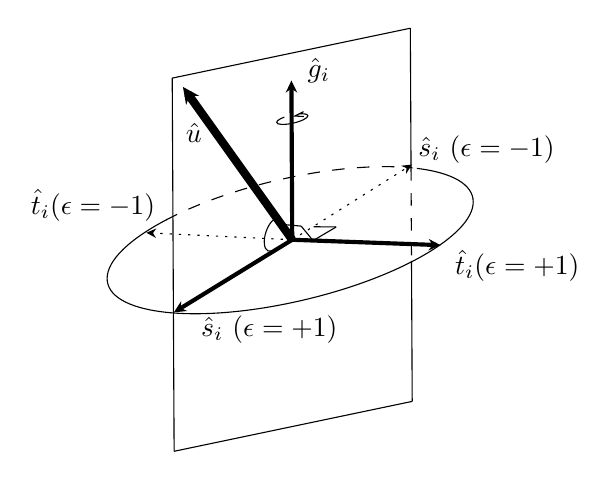
\begin{tikzpicture}[x=0.5pt,y=0.5pt,yscale=-1,xscale=1]
%uncomment if require: \path (0,348); %set diagram left start at 0, and has height of 348

%Straight Lines [id:da7916208743434348] 
\draw [line width=1.5]    (325.78,157.42) -- (243.69,207.79) ;
\draw [shift={(240.28,209.89)}, rotate = 328.47] [fill={rgb, 255:red, 0; green, 0; blue, 0 }  ][line width=0.08]  [draw opacity=0] (8.75,-4.2) -- (0,0) -- (8.75,4.2) -- (5.81,0) -- cycle    ;
%Straight Lines [id:da6063053587743079] 
\draw [line width=1.5]    (325.78,157.42) -- (429.04,161.18) ;
\draw [shift={(433.04,161.33)}, rotate = 182.09] [fill={rgb, 255:red, 0; green, 0; blue, 0 }  ][line width=0.08]  [draw opacity=0] (8.75,-4.2) -- (0,0) -- (8.75,4.2) -- (5.81,0) -- cycle    ;
%Straight Lines [id:da8584098766750565] 
\draw [line width=1.5]    (325.78,157.42) -- (325.22,46.36) ;
\draw [shift={(325.2,42.36)}, rotate = 449.71] [fill={rgb, 255:red, 0; green, 0; blue, 0 }  ][line width=0.08]  [draw opacity=0] (8.75,-4.2) -- (0,0) -- (8.75,4.2) -- (5.81,0) -- cycle    ;
%Straight Lines [id:da36750414352491156] 
\draw  [dash pattern={on 0.84pt off 2.51pt}]  (325.78,157.42) -- (409.76,104.66) ;
\draw [shift={(412.3,103.06)}, rotate = 507.86] [fill={rgb, 255:red, 0; green, 0; blue, 0 }  ][line width=0.08]  [draw opacity=0] (7.14,-3.43) -- (0,0) -- (7.14,3.43) -- (4.74,0) -- cycle    ;
%Straight Lines [id:da051548852230852926] 
\draw  [dash pattern={on 0.84pt off 2.51pt}]  (325.78,157.42) -- (223.36,152.49) ;
\draw [shift={(220.36,152.35)}, rotate = 362.75] [fill={rgb, 255:red, 0; green, 0; blue, 0 }  ][line width=0.08]  [draw opacity=0] (7.14,-3.43) -- (0,0) -- (7.14,3.43) -- (4.74,0) -- cycle    ;
%Straight Lines [id:da17659245242461763] 
\draw [line width=3]    (325.78,157.42) -- (276.96,89.13) -- (250.31,51.86) ;
\draw [shift={(246.82,46.98)}, rotate = 414.43] [fill={rgb, 255:red, 0; green, 0; blue, 0 }  ][line width=0.08]  [draw opacity=0] (11.97,-5.75) -- (0,0) -- (11.97,5.75) -- (7.95,0) -- cycle    ;
%Straight Lines [id:da48871347567863976] 
\draw    (341.17,148.01) -- (357.58,148.17) ;
%Straight Lines [id:da5947811121524507] 
\draw    (340.86,158.03) -- (357.58,148.17) ;
%Straight Lines [id:da18808003722282884] 
\draw    (318.62,146.33) -- (332.25,147.55) ;
%Straight Lines [id:da3929565984820087] 
\draw    (332.25,147.55) -- (340.86,158.03) ;
%Shape: Arc [id:dp1302171161481871] 
\draw  [draw opacity=0] (311.27,165.16) .. controls (311.04,165.28) and (310.81,165.38) .. (310.58,165.46) .. controls (306.98,166.74) and (304.84,162.5) .. (305.8,156) .. controls (306.72,149.85) and (310.07,143.88) .. (313.48,142.17) -- (312.33,153.69) -- cycle ; \draw   (311.27,165.16) .. controls (311.04,165.28) and (310.81,165.38) .. (310.58,165.46) .. controls (306.98,166.74) and (304.84,162.5) .. (305.8,156) .. controls (306.72,149.85) and (310.07,143.88) .. (313.48,142.17) ;
%Shape: Arc [id:dp4658593680079681] 
\draw  [draw opacity=0] (415.85,105.83) .. controls (440.9,108.83) and (456.52,117.16) .. (456.59,130) .. controls (456.72,155.04) and (397.59,187.75) .. (324.53,203.07) .. controls (251.47,218.39) and (192.14,210.5) .. (192.01,185.46) .. controls (191.94,172.1) and (208.74,156.56) .. (235.52,142.64) -- (324.3,157.73) -- cycle ; \draw   (415.85,105.83) .. controls (440.9,108.83) and (456.52,117.16) .. (456.59,130) .. controls (456.72,155.04) and (397.59,187.75) .. (324.53,203.07) .. controls (251.47,218.39) and (192.14,210.5) .. (192.01,185.46) .. controls (191.94,172.1) and (208.74,156.56) .. (235.52,142.64) ;
%Shape: Arc [id:dp7085048189876144] 
\draw  [draw opacity=0][dash pattern={on 4.5pt off 4.5pt}] (234.57,143.14) .. controls (258.09,130.76) and (289.52,119.63) .. (324.07,112.39) .. controls (358.2,105.23) and (389.34,103.14) .. (412.84,105.5) -- (324.3,157.73) -- cycle ; \draw  [dash pattern={on 4.5pt off 4.5pt}] (234.57,143.14) .. controls (258.09,130.76) and (289.52,119.63) .. (324.07,112.39) .. controls (358.2,105.23) and (389.34,103.14) .. (412.84,105.5) ;
%Straight Lines [id:da5865544576762574] 
\draw    (411.14,4.55) -- (411.65,105.77) ;
%Straight Lines [id:da7590207701341669] 
\draw    (239.07,40.6) -- (240.43,310.29) ;
%Straight Lines [id:da790374687044014] 
\draw    (239.07,40.6) -- (411.14,4.55) ;
%Straight Lines [id:da17494293181301823] 
\draw    (240.43,310.29) -- (412.5,274.23) ;
%Straight Lines [id:da5701402858596814] 
\draw    (411.99,172.73) -- (412.5,274.23) ;
%Straight Lines [id:da2349258321762262] 
\draw  [dash pattern={on 4.5pt off 4.5pt}]  (411.65,105.77) -- (411.99,172.73) ;
%Shape: Arc [id:dp4799622522622564] 
\draw  [draw opacity=0] (330.58,66.45) .. controls (334.42,66.13) and (337.09,66.63) .. (337.1,67.85) .. controls (337.1,69.54) and (332.07,71.96) .. (325.85,73.26) .. controls (319.63,74.57) and (314.58,74.26) .. (314.58,72.57) .. controls (314.57,71.45) and (316.78,70.01) .. (320.09,68.78) -- (325.84,70.21) -- cycle ; \draw   (330.58,66.45) .. controls (334.42,66.13) and (337.09,66.63) .. (337.1,67.85) .. controls (337.1,69.54) and (332.07,71.96) .. (325.85,73.26) .. controls (319.63,74.57) and (314.58,74.26) .. (314.58,72.57) .. controls (314.57,71.45) and (316.78,70.01) .. (320.09,68.78) ;
\draw   (333.97,64.87) -- (327.59,67.99) -- (334.21,68.38) ;

% Text Node
\draw (441.66,162.98) node [anchor=north west][inner sep=0.75pt]    {$\hat{t}_{i}( \epsilon =+1)$};
% Text Node
\draw (258,210.4) node [anchor=north west][inner sep=0.75pt]    {$\hat{s}_{i} \ ( \epsilon =+1)$};
% Text Node
\draw (415,80.4) node [anchor=north west][inner sep=0.75pt]    {$\hat{s}_{i} \ ( \epsilon =-1)$};
% Text Node
\draw (135,119.4) node [anchor=north west][inner sep=0.75pt]    {$\hat{t}_{i}( \epsilon =-1)$};
% Text Node
\draw (247,71.4) node [anchor=north west][inner sep=0.75pt]    {$\hat{u}$};
% Text Node
\draw (335,24.4) node [anchor=north west][inner sep=0.75pt]    {$\hat{g}_{i}$};
\end{tikzpicture}

    \caption{Vector representation at singular gimble state}
    \label{fig:tikCMG}
\end{figure}

\begin{figure}[h]
\centering
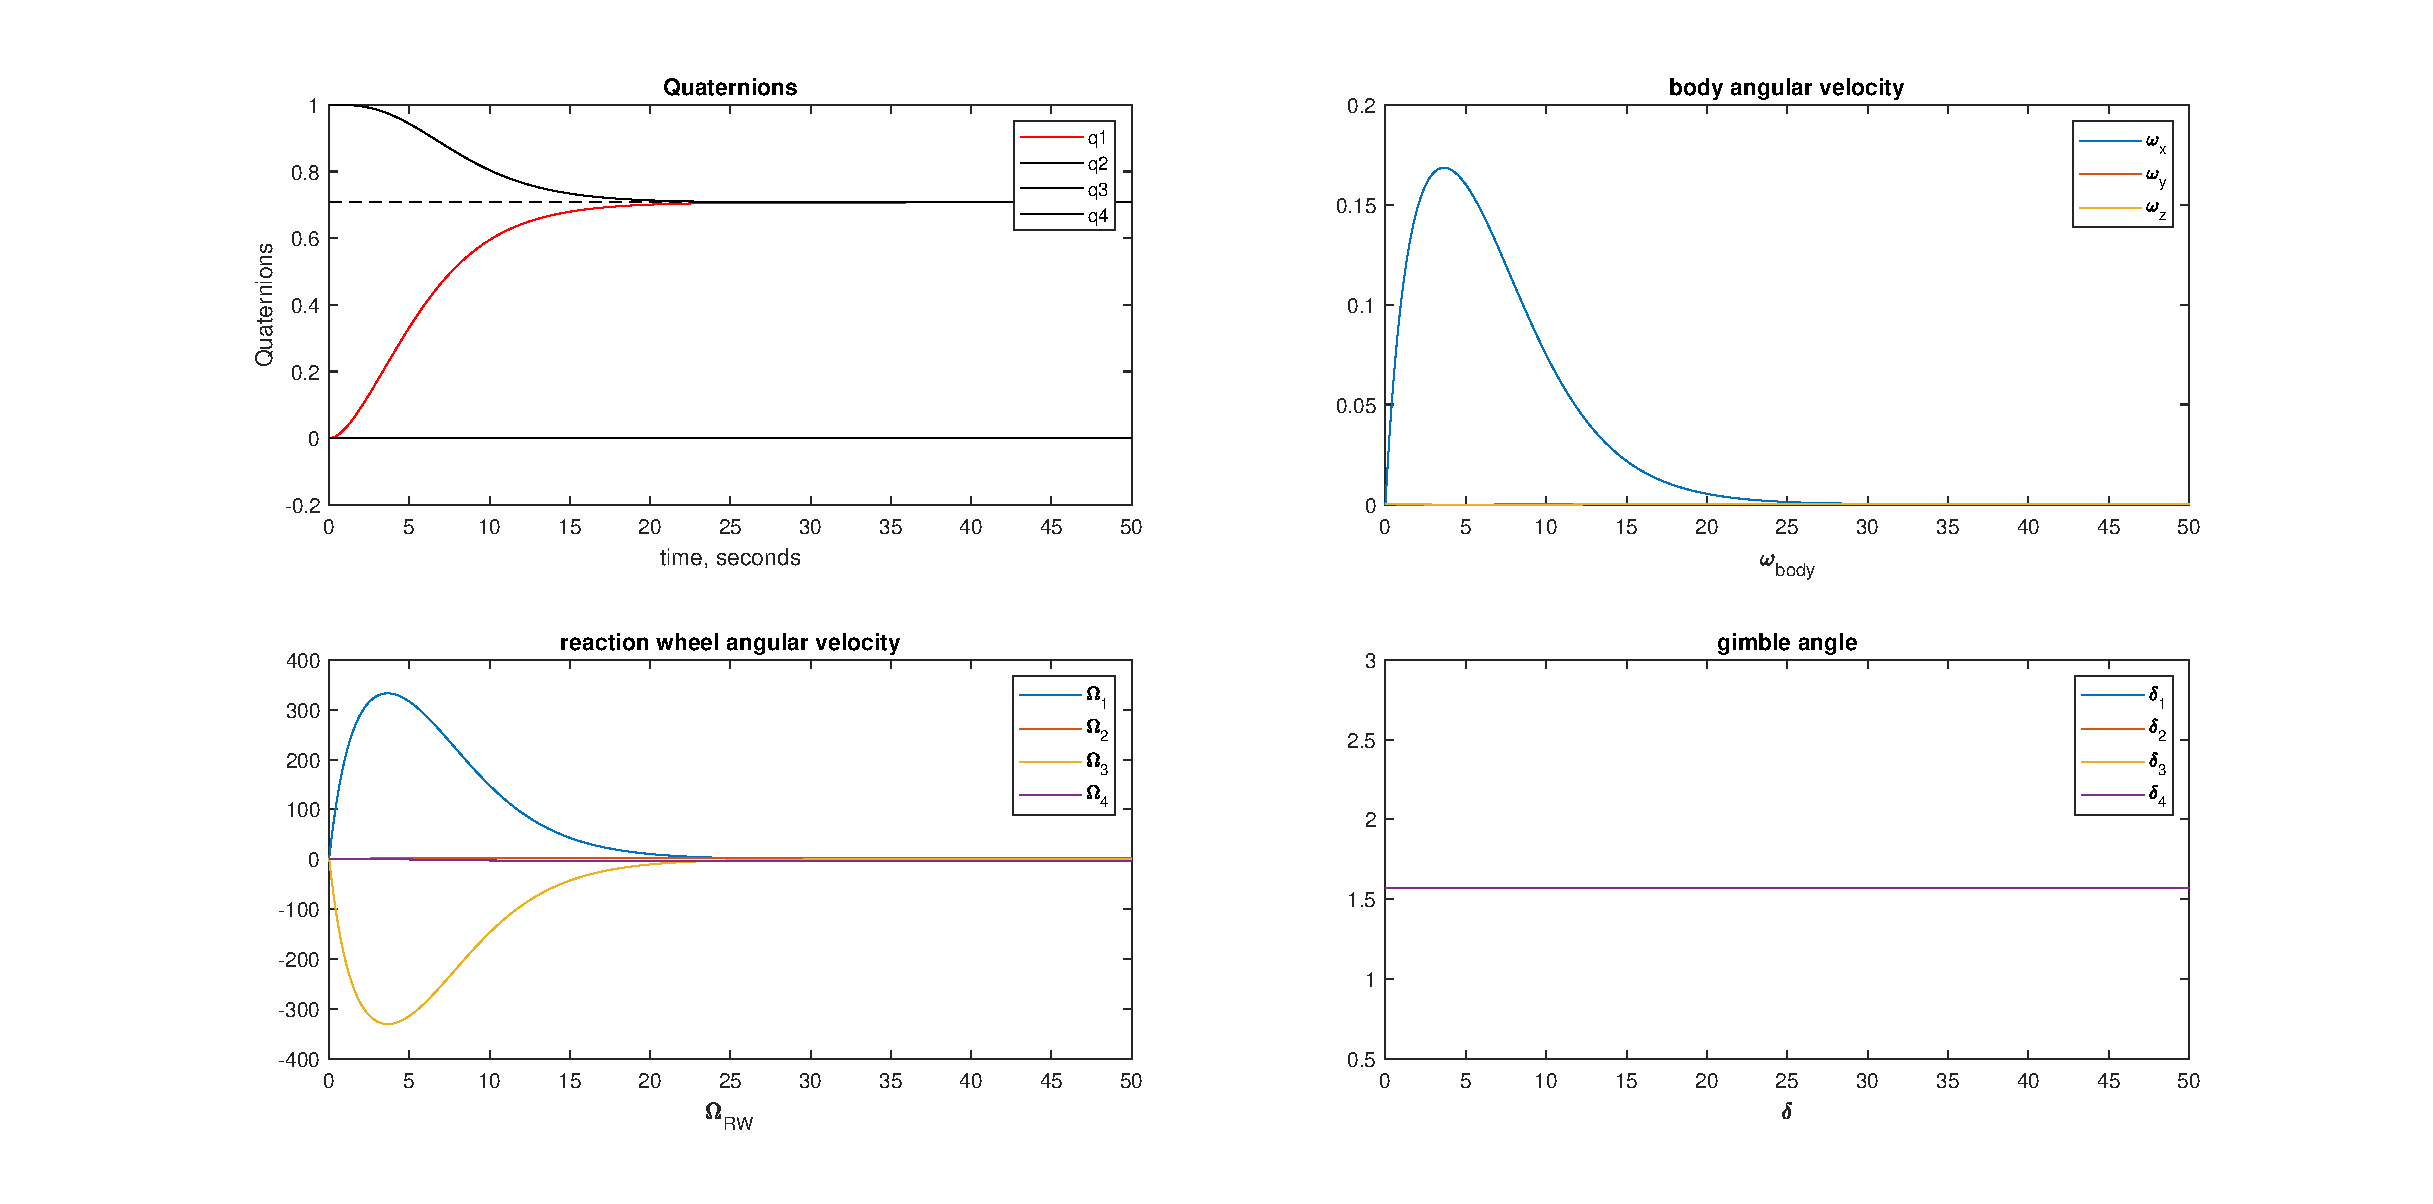
\includegraphics[scale=0.5]{figures/fig4.eps}
\end{figure}

\section{Page layout}

The page is fixed at the dimensions of an A4 paper, therefore you have to print your thesis on A4 paper to obtain the best results. The font dimension is fixed at 11\, pt. The text column and the margins are chosen to fill to the best an A4 paper while keeping a reasonable line length (396\, pt) for a good readability. The text height and the text width are in golden ratio (\textasciitilde 1.6180) as well as the outer and inner margins in a two-side document after binding margin removal. Also the top margin (excluding the header) and bottom margin are in the golden ratio. In Fig.~\ref{layout} a sketch of the \textsf{sapthesis} page layout is shown. \acrlong{vscmg}

\begin{figure}[h]
\centering
\setlength{\unitlength}{0.27mm}
\begin{picture}(420,297)(-210,0)
\polyline(-210,0)(210,0)(210,297)(-210,297)(-210,0)
\Line(0,0)(0,297)
\put(27.05,37.4){\polygon(0,0)(139.2,0)(139.2,223.8)(0,223.8)}
\put(-27.05,37.4){\polygon(0,0)(-139.2,0)(-139.2,223.8)(0,223.8)}
\put(27.05,268.16){\polygon(0,0)(139.2,0)(139.2,4.22)(0,4.22)}
\put(-27.05,268.16){\polygon(0,0)(-139.2,0)(-139.2,4.22)(0,4.22)}
\end{picture}
\caption{Page layout scheme of \textsf{sapthesis class} using a zero binding margin.}
\label{layout}
\end{figure}


\section{Page style}

The captions have a smaller font respect to the text and the label is in boldface. The appearance of the margin notes has been improved.
They have the same font dimension of the footnotes and are typed in italics.
Moreover I defined a new command to typeset margin note aligned to the left on the right page and vice versa on the left page.
Notice that if a binding margin greater than 1.5\, cm is used, the dimensions of the margin notes become too small and very ugly.
Do not use them in this case.

The mathematical objects, figures and tables are numbered within the chapters (e.g. 1.1, 1.2,\ldots for the first chapter, 2.1, 2.2 for the second one and so on\ldots). See for example the number of this simple equation
\begin{equation}
x_{1,2}=\frac{-b\pm\sqrt{b^2-4ac}}{2a}
\end{equation}


The title page is automatically composed when the \texttt{\bs maketitle} command is given.
The parameters needed for the title page, author, title, etc\ldots , are supplied by dedicated commands explained in the next section.
Two copies of the university logo in \texttt{pdf} format, one for color printing and the other one for black and white printing, are supplied in the \textsf{sapthesis} package. They are shown in Fig.~\ref{fig:largenenough}.

\begin{figure}
\centering
\includegraphics[width=0.7\textwidth]{sapienza-MLred-pos}\\[3ex]
\includegraphics[width=0.7\textwidth]{sapienza-MLblack-pos}
\caption{Logo of the Sapienza -- University of Rome.}
\label{fig:largenenough}
\end{figure}



\section{About figures and tables}

As regards the image formats, please use vector images as much as possible! Use jpg images only for photographs! pdf\LaTeX\ supports the pdf, jpg and png formats.

A very simple table is show in Tab.~\ref{tab:letters}. Remember to typeset
always the table caption above the table. Do not use vertical lines.

\begin{table}
\caption{This is a simple table.}
\label{tab:letters}
\centering
\begin{tabular}{lcc}
\toprule
Letter & Test & Test \\
\midrule
A & C & E \\
B & D & F \\
\bottomrule
\end{tabular}
\end{table}


\section{A section}

In this manual you can skip the gray text because it is just dummy text.



\section{Another section}

In this manual you can skip the gray text because it is just dummy text.



%  Controller Design
\chapter{Controller Design}
\label{chap:4}
In the interest of trajectory tracking and regulation maneuver during mission life cycle of spacecraft, suitable controller law is crucial choice ensuring accuracy and stability in presence of disturbances. Bearing in mind that the equation of motion for a spacecraft equipped with VSCMG units are highly complex and nonlinear in nature. It is clear that \autoref{eqn:EOM_FULL} is time varying function of change in moment of inertia, gimbal angle, reaction wheel and gimbal angular velocity and acceleration. Nested control architecture is realized. As shown in \autoref{fig:control_architecture}, Outer feedback loop deals with evaluation of torques $\tau_{c}$ based on state error with the intention of regulation or trajectory tracking. Furthermore, inner control loop to produce required torque from individual actuators. RW generates torque by accelerating flywheel whereas in case CMG, torque is proportional to angular momentum of RW and gimbal velocity. The idea is to find out particular combination of gimbal velocities and RW accelerations in order to produce required torque demanded by outer loop with strong emphasis on avoiding singularity.
\begin{figure}[!h]
    \centering
    \tikzstyle{block} = [draw, fill=blue!0, rectangle, 
    minimum height=3em, minimum width=5em,align=center]
\tikzstyle{sum} = [draw, fill=blue!0, circle, node distance=1cm]
\tikzstyle{input} = [coordinate]
\tikzstyle{tmp} = [coordinate]
\tikzstyle{output} = [coordinate]
\tikzstyle{pinstyle} = [pin edge={to-,thin,black}]

\begin{tikzpicture}[auto, node distance=2cm,>=latex']
% Boxing and labelling noise shapers
	\draw [color=black,thick,fill={rgb:black,1;white,30}](6.2,1.2) rectangle (11.2,-0.8);
	\node at (6,1) [below=1mm, right=2mm] {{Spacecraft Bus}};
	
    \node [input, name=input] {};
    \node [sum, right of=input](sum) {};
    \node [block, right of=sum, name=ctrl,node distance=1.5cm]
        {Control \\ Law};
    \node [block, right of=ctrl, name=str,node distance=2.5cm]
        {Steering \\ Law};
    \node [block, right of=str,node distance=2.5cm] (cmg)
        {VSCMG \\ Cluster};
    \node [block, right of=cmg,node distance=2.5cm] (sys)
        {Platform \\ Dynamics};
    \node [output,right of=sys,node distance=2cm] (output){};
    
    
    \draw [draw,->] (input) -- node {$r$} (sum);
    \draw[->](sum)--node {$e$}(ctrl);
    \draw[->](ctrl)--node {$\tau_c$}(str);
    \draw[->](str)--node {}(cmg);
    \draw[->](cmg)--node {$\tau_{a}$}(sys);
    \draw[->](sys)-- node [name=y] {$y$}(output);
    \node[tmp,below of=sys,node distance=1.5cm](fo1){};
    \node[tmp,below of=y,node distance=2.5cm](fo2){};
    \draw[->](y)--(fo2)-|node[pos=0.99] {$-$} 
        node [near start] {Spacecraft State feedback}(sum);
    \draw[->](sys)--(fo1)-|node [near start] {VSCMG State feedback}(str);


\end{tikzpicture}

    %\includegraphics{}
    \caption{VSCMG Spacecraft Control Architecture}
    \label{fig:control_architecture}
\end{figure}

\section{Lyapunov Stability Method}
Lyapunov stability is widely used methods for continuous time nonlinear systems, two methods proposed by Aleksandr Lyapunov in1892 are indirect method in which behavior linearized system about equilibrium point is examined whereas direct method to verify stability of nonlinear system by inspecting evaluation of "lyapunov function" an energy like positive definite function composed of \ system states. If the carefully constructed scalar function decreases over time, the system under study is proved to be stable. It is possible to realize controller which dissipates selected scalar function.

Consider continuous, time-invariant nonlinear system with state $\displaystyle x$ and control input $\displaystyle u$.
\begin{equation*}
\dot{x} =f( x,u)
\end{equation*}
The idea behind Lyapunov direct method is crafting positive definite scalar function $\displaystyle \mathcal{V}( x)$ and substituting $\displaystyle u=u( x)$ making it closed loop dynamical system such a way that with derived controller the derivative $\displaystyle \dot{\mathcal{V}}( x)$ becomes negative. Stability critaria is
\begin{equation}
 \begin{aligned}
\mathcal{V}( x)  >0 & & \\
\dot{\mathcal{V}}( x) < 0 & & \\
\mathcal{V}( x)\rightarrow \infty , & & ||x||\rightarrow \infty 
\end{aligned}
\label{eqn:lyp_cond}
\end{equation}


If selected scalar function with derived controller satisfies \autoref{eqn:lyp_cond} then system is said to be asymptotically stable. 



\section{Model based Controller Design}
A control law must be designed in such a way that it guaranties asymptotic stability of states, by shifting global equilibrium to desired state. For external feedback control loop let $\displaystyle \mathcal{F}_{d}$ be desired body fixed rotating frame and spacecraft current state body fixed reference frame $\displaystyle \mathcal{F}_{b}$ described with respect to inertial frame $\displaystyle \mathcal{F}_{i}$. As described in \autoref{chap:2} let $\displaystyle \omega $ be the angular velocity of $\displaystyle \mathcal{F}_{b}$ and $\displaystyle q=q_{0} +q_{v}$ be current attitude of $\displaystyle \mathcal{F}_{b}$. Lets recall rotation matrix from $\displaystyle \mathcal{F}_{i}$ to $\displaystyle \mathcal{F}_{b}$

\begin{equation}
\mathbf{R} (\mathbf{q} )=\left( q^{2}_{0} -\mathbf{q}^{T}_{v}\mathbf{q}_{v}\right)\mathbf{I}_{3\times 3} +2\mathbf{q}_{v}\mathbf{q}^{T}_{v} +2q_{0}\mathbf{q}^{\times }
\end{equation}Similarly, \ $\displaystyle q_{d} =q_{d,0} +q_{d,v}$ the attitude quaternion of $\displaystyle \mathcal{F}_{d}$ and $\displaystyle ^{i} \omega _{d}$ be angular velocity of desired reference frame. The rotation matrix which transforms $\displaystyle \mathcal{F}_{i}$ to $\displaystyle \mathcal{F}_{b}$ is

\begin{equation}
\mathbf{R} (\mathbf{q}_{d} )=\left( q^{2}_{0,d} -\mathbf{q}^{T}_{v,d}\mathbf{q}_{v,d}\right)\mathbf{I}_{3\times 3} +2\mathbf{q}_{v,d}\mathbf{q}^{T}_{v,d} +2q_{0,d}\mathbf{q}^{\times }_{d}
\end{equation}Attitude of $\displaystyle \mathcal{F}_{b}$ described with respect to $\displaystyle \mathcal{F}_{b}$ can be considered as deviation in tracking, hence with tracking error quaternion $\displaystyle q_{e} =q_{e,0} +q_{e,v}$ rotation matrix among body and desired frame is expressed as\begin{equation}
\mathbf{R} (\mathbf{q}_{e} )=\left( q^{2}_{0,e} -\mathbf{q}^{T}_{e,d}\mathbf{q}_{e,d}\right)\mathbf{I}_{3\times 3} +2\mathbf{q}_{e,d}\mathbf{q}^{T}_{e,d} +2q_{0,e}\mathbf{q}^{\times }_{e}
\end{equation}recalling from chap error quaternion representation in vectorial and eigen axis from
\begin{equation}
\begin{pmatrix}
\mathbf{q}_{e,0}\\
q_{v,e}
\end{pmatrix} =\begin{pmatrix}
\cos( \varepsilon /2) \ \\
\mathbf{\hat{e}}\sin( \varepsilon /2)
\end{pmatrix} =\begin{pmatrix}
q_{0} q_{d,0} +\mathbf{q}^{T}\mathbf{q}_{d}\\
-q_{0} q_{d,v} +q_{d,0} q_{v} -q_{v} \times q_{d,v}
\end{pmatrix}
\end{equation}
When current attitude and desired attitude are same, angular displacement is $\displaystyle \varepsilon $ becomes zero making error quaternion

\begin{equation}
\mathbf{q}_{e} =\begin{pmatrix}
q_{e,0}\\
q_{v,e}
\end{pmatrix} =\begin{pmatrix}
1\\
\mathbf{0}
\end{pmatrix}
\end{equation}Angular velocity tracking error $\displaystyle \omega _{e}$ is angular velocity of body frame with respect to desired frame $\displaystyle \mathcal{F}_{d}$ can be expressed in $\displaystyle \mathcal{F}_{b}$ as 
\label{eqn:qe_zero}
\begin{equation*}
\omega _{e} =\omega -\mathbf{R} (\mathbf{q}_{e} )^{i} \omega _{d} =\omega -\omega _{d}
\end{equation*}
here $\displaystyle \omega _{d}$ is angular velocity of desired frame with respect to current body frame. The quaternion kinematics for error tracking expressed in body frame
\begin{equation}
\begin{aligned}
\dot{\mathbf{q}_{e}} & =\frac{1}{2}\begin{bmatrix}
-\mathbf{\omega }_{e} \cdot q_{e,v}\\
q_{e,0}\mathbf{\omega }_{e} -q^{\times }_{e,v}
\end{bmatrix}\\
\mathbf{q}_{e} & =\frac{1}{2}\begin{bmatrix}
0 & -\mathbf{\omega }_{e}\\
\mathbf{\omega }_{e} & -\mathbf{\omega }^{\times }_{e}
\end{bmatrix}\begin{bmatrix}
q_{e,0}\\
q_{e,v}
\end{bmatrix}
\end{aligned}
\end{equation}
Similar approach will be used to derive ``Reward Function'' for training Neural Netrwork policy with \acrfull{rl} methods.
\subsection{The Lyapunov Candidate Function}
Based on previously developed analogy of quaternion tracking error and angular velocity tracking error, for shifted target equilibrium candidate Lyapunov function is selected as

\begin{equation}
\mathcal{V} =\frac{1}{2} \omega ^{T}_{e}\mathbf{K}^{-1} J\omega _{e} +q_{e,v} q^{T}_{e,v} +( q_{e,0} -1)^{2}
\label{eqn:lyp_first}
\end{equation}
Here. $\displaystyle J$ is inertia tensor of complete spacecraft and function and $\displaystyle \mathbf{K}^{-1}_{3\times 3}$ is positive definite matrix. consequently $\displaystyle \mathcal{V}$ guaranties to be positive definite since all the terms in \autoref{eqn:lyp_first} are in quadratic form. From \autoref{eqn:qe_zero} we can deduce that that Candidate becomes zero when velocity tracking error and quaternion error becomes zero. With unit norm quaternion property
\begin{equation}
q^{2}_{e,0} +q_{e,v} q^{T}_{e,v} =1
\end{equation}
\begin{equation}
( q_{e,0} -1)^{2} +q_{e,v} q^{T}_{e,v} =( q_{e,0} -1)^{2} +1-q^{2}_{e,0} =2( 1-q_{e,0})
\label{eqn:unit_norm_quat_rearanged}
\end{equation}
Using above relation Lyapunov Candidate function is reduced to
\begin{equation}
\mathcal{V} =\frac{1}{2} \omega ^{T}_{e}\mathbf{K}^{-1} J\omega _{e} +2( 1-q_{e,0})
\label{eqn:lyp_first_reduced}
\end{equation}
Another popular candidate function selected for regulation is purely based on kinetic energy of spacecraft which is
\begin{equation}
\mathcal{V} =\frac{1}{2} \omega ^{T} J\omega 
\end{equation}

\subsection{Stability Analysis}
In order to evaluate stability of system, Candidate function derivative $\displaystyle \dot{\mathcal{V}}$ should be negative which guaranties asymptotic stability of system, in this case chosen function is
\begin{equation}
\mathcal{V} =\frac{1}{2} \omega ^{T}_{e}\mathbf{K}^{-1}_{q} J\omega _{e} +2( 1-q_{e,0})
\end{equation}
taking time derivative of candidate function
\begin{equation}
\dot{\mathcal{V}} =\frac{1}{2} \omega ^{T}_{e}\mathbf{K}^{-1}_{q}\dot{J} \omega _{e} +\omega ^{T}_{e}\mathbf{K}^{-1}_{q} J\dot{\omega }_{e} -2\dot{q}_{e,0}
\end{equation}
Substituting derivative of inertia tensor in above expression we have
\begin{equation}
\begin{aligned}
\dot{\mathcal{V}} & =\frac{1}{2}\left( J^{s}_{CMG} -J^{t}_{CMG}\right) \omega ^{T}_{e}\mathbf{K}^{-1}_{q}\sum ^{n}_{k=1}\dot{\delta }_{k}[\hat{t}_{k} \ \hat{s}_{k} +\hat{s}_{k} \ \hat{t}_{k}] \cdotp \omega _{e}\\
 & -\ \left( J^{s}_{CMG} -J^{t}_{CMG}\right) \omega ^{T}_{e}\mathbf{K}^{-1}_{q}\sum ^{n}_{k=1}\dot{\delta }_{k}[\hat{t}_{k} \ \hat{s}_{k} +\hat{s}_{k} \ \hat{t}_{k}] \cdotp \omega \\
 & -\ \omega ^{T}_{e}\mathbf{K}^{-1}_{q}[ \omega \times J\omega ]\\
 & -\ \omega ^{T}_{e}\mathbf{K}^{-1}_{q}\left[ J^{s}_{W}\sum ^{n}_{k=1} \ \dot{\Omega }_{k} \ \hat{s}_{k} +\ J^{s}_{W} \ \sum ^{n}_{k=1} \Omega _{k}\dot{\delta }_{k} \ \hat{t}_{k} +J^{s}_{W} \omega \times \sum ^{n}_{k=1} \ \Omega _{k} \ \hat{s}_{k}\right]\\
 & -\ \omega ^{T}_{e}\mathbf{K}^{-1}_{q}\left[ J^{g}_{CMG}\sum ^{n}_{k=1} \ \ddot{\delta }_{k} \ \hat{g}_{k} +\ J^{g}_{CMG} \ \omega \times \sum ^{n}_{k=1}\dot{\delta }_{k} \ \hat{g}_{k}\right]\\
 & -\ \omega ^{T}_{e}\mathbf{K}^{-1}_{q} J\dot{\omega }_{d} +\omega _{e} q^{T}_{e}
\end{aligned}
\label{eqn:lyp_deriv_expanded1}
\end{equation}
In order to ensure $\displaystyle \dot{\mathcal{V}} < 0$, from expression above taking $\displaystyle \omega _{e}$ common and introducing new positive definite matrix $\displaystyle \mathbf{K}_{w}$ such a way that \autoref{eqn:lyp_deriv_expanded1} becomes
\begin{equation}
\dot{\mathcal{V}} =-\ \omega ^{T}_{e}\mathbf{K}^{-1}_{q}\mathbf{K}_{w} \omega _{e}
\end{equation}
\begin{equation}
\begin{aligned}
-\mathbf{K}^{-1}_{q}\mathbf{K}_{w} \omega _{e} & =-\frac{1}{2}\left( J^{s}_{CMG} -J^{t}_{CMG}\right)\mathbf{K}^{-1}_{q}\sum ^{n}_{k=1}\dot{\delta }_{k}[\hat{t}_{k} \ \hat{s}_{k} +\hat{s}_{k} \ \hat{t}_{k}] \cdotp ( \omega +\omega _{d})\\
 & -\ \mathbf{K}^{-1}_{q}[ \omega \times J\omega ]\\
 & -\ \mathbf{K}^{-1}_{q}\left[ J^{s}_{W}\sum ^{n}_{k=1} \ \dot{\Omega }_{k} \ \hat{s}_{k} +\ J^{s}_{W} \ \sum ^{n}_{k=1} \Omega _{k}\dot{\delta }_{k} \ \hat{t}_{k} +J^{s}_{W} \omega \times \sum ^{n}_{k=1} \ \Omega _{k} \ \hat{s}_{k}\right]\\
 & -\ \mathbf{K}^{-1}_{q}\left[ J^{g}_{CMG}\sum ^{n}_{k=1} \ \ddot{\delta }_{k} \ \hat{g}_{k} +\ J^{g}_{CMG} \ \omega \times \sum ^{n}_{k=1}\dot{\delta }_{k} \ \hat{g}_{k}\right]\\
 & -\ \mathbf{K}^{-1}_{q} J\dot{\omega }_{d} +q_{e}
\end{aligned}
\label{eqn:lyp_deriv_withK}
\end{equation}
Since $\displaystyle \mathbf{K}^{-1}_{q}$ appears in both sides, \autoref{eqn:lyp_deriv_withK} can be expressed as 
\begin{equation}
\begin{aligned}
 & \frac{1}{2}\left( J^{s}_{CMG} -J^{t}_{CMG}\right)\sum ^{n}_{k=1}\dot{\delta }_{k}[\hat{t}_{k} \ \hat{s}_{k} +\hat{s}_{k} \ \hat{t}_{k}] \cdotp ( \omega +\omega _{d})\\
 & +\ J^{s}_{W}\sum ^{n}_{k=1} \ \dot{\Omega }_{k} \ \hat{s}_{k} +\ J^{s}_{W} \ \sum ^{n}_{k=1} \Omega _{k}\dot{\delta }_{k} \ \hat{t}_{k}\\
 & +\ J^{g}_{CMG}\sum ^{n}_{k=1} \ \ddot{\delta }_{k} \ \hat{g}_{k} +\ J^{g}_{CMG} \ \omega \times \sum ^{n}_{k=1}\dot{\delta }_{k} \ \hat{g}_{k}\\
 & =\ \mathbf{K}_{w} \omega _{e} +\mathbf{K}_{q} q_{e} -J\dot{\omega }_{d} -\omega \times \left[ J\omega +J^{s}_{W}\sum ^{n}_{k=1} \ \Omega _{k} \ \hat{s}_{k}\right]
\end{aligned}
\label{eqn:lyp_deriv_fin1}
\end{equation}
Substituting \autoref{eqn:lyp_deriv_fin1} in  \autoref{eqn:EOM_FULL} complete nonlinear dynamical equation
\begin{equation}
J\dot{\omega _{e}} +\dot{J} \omega _{e} =\ -\mathbf{K}_{w} \omega _{e} -\mathbf{K}_{q} q_{e}
\label{eqn:error_tracking_eom}
\end{equation}
\autoref{eqn:error_tracking_eom} is error tracking control of VSCMG, we can see it resembles proportional derivative control, $\displaystyle \mathbf{K}_{q}$ being proportional gain while $\displaystyle \mathbf{K}_{w}$ can be considered as derivative gain matrix.In terms of control torque $\displaystyle u$ expression is 
\begin{tcolorbox}
\begin{equation}
u=-\mathbf{K}_{w} \omega _{e} -\mathbf{K}_{q} q_{e}
\end{equation}
\end{tcolorbox}

Expression assures asymptotic stability of $\displaystyle \omega _{e}$, In order to make sure \autoref{eqn:lyp_first} satisfies Lyapunov criterion, and guarantying asymptotic stability of all the states as we know $\displaystyle \omega _{e,\infty }\rightarrow 0$ thus $\displaystyle \dot{\omega }_{e,\infty }\rightarrow 0$ we can demonstrate the quaternion vector components tends to zero and scalar becomes 1 thus making 
\begin{equation}
\mathbf{K}_{q} q_{e,\infty } =0
\end{equation}
From argument above we can ensure that \ $\displaystyle q_{e,\infty }$ tends to zero thus \autoref{eqn:lyp_first} satisfies  Lyapunov  criterion for all states. Now, rearranging control variables in order to have control torque that can be generated internally all momentum exchange devices is expressed as
\begin{equation*}
\begin{aligned}
u & =\frac{1}{2}\left( J^{s}_{CMG} -J^{t}_{CMG}\right)\sum ^{n}_{k=1}\dot{\delta }_{k}[\hat{t}_{k} \ \hat{s}_{k} +\hat{s}_{k} \ \hat{t}_{k}] \cdotp ( \omega +\omega _{d})\\
 & +\ J^{s}_{W}\sum ^{n}_{k=1} \ \dot{\Omega }_{k} \ \hat{s}_{k} +\ J^{s}_{W} \ \sum ^{n}_{k=1} \Omega _{k}\dot{\delta }_{k} \ \hat{t}_{k}\\
 & +\ J^{g}_{CMG}\sum ^{n}_{k=1} \ \ddot{\delta }_{k} \ \hat{g}_{k} +\ J^{g}_{CMG} \ \omega \times \sum ^{n}_{k=1}\dot{\delta }_{k} \ \hat{g}_{k}
\end{aligned}
\end{equation*}
Consequently. demand torque required to make $\displaystyle \omega _{e,\infty }$ and $\displaystyle q_{e,\infty }$ tends to zero is
\begin{equation}
u =\mathbf{K}_{w} \omega _{e} +\mathbf{K}_{q} q_{e} -J\dot{\omega }_{d} -\ \omega \times \left[ J\omega +J^{s}_{W}\sum ^{n}_{k=1} \ \Omega _{k} \ \hat{s}_{k}\right]
\end{equation}
Making close loop dynamics of Spacecraft with VSCMG suitable for both trajectory tracking and regulation becomes
\begin{equation}
\dot{J\omega } +\frac{1}{2}\dot{J} \omega _{e} +\omega \times \left[ J\omega +^{s}_{W}\sum ^{n}_{k=1} \ \Omega _{k} \ \hat{s}_{k}\right] =-u
\end{equation}

\section{Steering Law}
In order to generate torque required to reach desired state, appropriate signal must be provided to momentum exchange devices present in spacecraft. VSCMG produce torque using reaction wheel angular acceleration $\displaystyle \dot{\Omega }$, gimbal velocity $\displaystyle \dot{\delta }$ and gimbal acceleration $\displaystyle \ddot{\delta }$. In the interest of evaluating precise values taking into consideration for particular arrangement of generic number of VSCMG cluster.

Demand torque expression written in terms of momentum exchange devices given in equation can be expressed in matrix form for generic number of VSCMG units as
\begin{equation}
u=B\ddot{\delta } +C\dot{\delta } +D\dot{\Omega }
\label{eqn:steering_controller}
\end{equation}
here coefficient matrices $\displaystyle B_{3\times n}$, $\displaystyle C_{3\times n}$ and $\displaystyle D_{3\times n}$ are composed of 3 rows and $\displaystyle n$ columns as
\begin{equation}
\begin{aligned}
B & =J^{g}_{CMG}\sum ^{n}_{k=1} \ \hat{g}_{k}\\
B & =J^{g}_{CMG}\mathcal{G}_{g}
\end{aligned}
\end{equation}
\begin{equation}
\begin{aligned}
C & =\sum ^{n}_{k=1}\left[ J^{s}_{W} \ \Omega _{k} \ \hat{t}_{k} +\frac{1}{2}\left( J^{s}_{CMG} -J^{t}_{CMG}\right)[\hat{t}_{k} \ \hat{s}_{k} +\hat{s}_{k} \ \hat{t}_{k}] \cdotp ( \omega +\omega _{d}) +\ J^{g}_{CMG} \ \omega \times \ \hat{g}_{k}\right]\\
C & =J^{s}_{W} \ [ \Omega ]^{d}\mathcal{G}_{t} +\frac{1}{2}\left( J^{s}_{CMG} -J^{t}_{CMG}\right)\mathcal{G}_{st\omega ^{+}} +J^{g}_{CMG} \ \omega \times \mathcal{G}_{g}
\end{aligned}
\label{eqn:steerC_full}
\end{equation}
\begin{equation}
\begin{aligned}
D & =\sum ^{n}_{k=1} J^{s}_{W}\hat{s}_{k}\dot{\Omega }_{k}\\
D & =J^{s}_{W}\mathcal{G}_{s}
\end{aligned}
\end{equation}
where, direction cosines of gimbal spin and transverse axis are written as
\begin{equation*}
\mathcal{G}_{g} =\begin{bmatrix}
| & | &  & |\\
\hat{g}_{1} & \hat{g}_{2} & \dotsc  & \hat{g}_{n}\\
| & | &  & |
\end{bmatrix}_{3\times n}  \mathcal{G} t=\begin{bmatrix}
| & | &  & |\\
\hat{t}_{1} & \hat{t}_{2} & \dotsc  & \hat{t}_{n}\\
| & | &  & |
\end{bmatrix}_{3\times n}  \mathcal{G} s=\begin{bmatrix}
| & | &  & |\\
\hat{s}_{1} & \hat{s}_{2} & \dotsc  & \hat{s}_{n}\\
| & | &  & |
\end{bmatrix}_{3\times n}
\end{equation*}
\begin{equation*}
\mathcal{G} st\omega ^{+} =\begin{bmatrix}
| &  & |\\
[\hat{t}_{1}\hat{s}_{1} +\hat{s}_{1}\hat{t}_{1}] \cdotp ( \omega +\omega _{d}) & \dotsc  & [\hat{t}_{1}\hat{s}_{1} +\hat{s}_{1}\hat{t}_{1}] \cdotp ( \omega +\omega _{d})\\
| &  & |
\end{bmatrix}_{3\times n}
\end{equation*}Diagonal matrix is represented by brackets with superscript $\displaystyle [ \ ]^{d}$ as
\begin{equation*}
[ \Omega ]^{d} =\begin{bmatrix}
\Omega _{1} &  &  & 0\\
 & \Omega _{2} &  & \\
 &  & \ddots  & \\
0 &  &  & \Omega _{n}
\end{bmatrix}_{3\times n}
\end{equation*}
Neglecting smaller terms in \autoref{eqn:steerC_full}, $\displaystyle C$ becomes
\begin{equation}
C=J^{s}_{W}[ \Omega ]^{d}\mathcal{G}_{t}
\end{equation}
And for momentum wheel portion, keeping constant gimbal angle at all times makes $\displaystyle D$ constant, thus \autoref{eqn:steering_controller} is simplified as
\begin{equation}
\begin{aligned}
u & =\sum ^{n}_{k=1} J^{s}_{W}\hat{s}_{k}\dot{\Omega }_{k}\\
u & =D\dot{\Omega }_{k}
\end{aligned}
\label{eqn:mw_ik}
\end{equation}
\autoref{eqn:mw_ik} is considering only reaction wheel based control torques.Whereas keeping RW angular velocity $\displaystyle \dot{\Omega }$ constant and neglecting very small gimbal acceleration term, CMG based control is achieved as 
\begin{equation}
u=C[\dot{\delta }]^{d}
\label{eqn:cmg_control_only}
\end{equation}
\subsection{Reaction Wheel Optimization}
As seen earlier sections, VSCMG clusters gives ability to produced torques by only using Reaction Wheels as torque producing unit, and required torques can be realized by
\begin{equation}
u=D\dot{\Omega }
\end{equation}
Since number of equations 3 and are more than number of unknown variables due to the fact that more that there will be more than three reaction wheels present for the purpose redundancy. The solution has dimension $\displaystyle \mathcal{N}( D) =m-n$ degrees of freedom. Where number of equations $\displaystyle n=3$ and number of unknown variables $\displaystyle m >3$. There is no trivial solution for such problem and required solution can only be found with optimization criteria. In this case minimum norm criteria is used for RW acceleration. Let us define Lagrangian $\displaystyle \mathcal{L}$ and Lagrangian 
\begin{equation}
\mathcal{L}(\dot{\Omega }) =||\dot{\Omega } ||=\dot{\Omega }^{T}\dot{\Omega }
\end{equation}
In order to minimize $\displaystyle \min \ ||\dot{\Omega } ||$ for $\displaystyle u=D\dot{\Omega }$ by introducing Lagrangian multiplier $\displaystyle \lambda $
\begin{equation}
f=\dot{\Omega }^{T}\dot{\Omega } +\lambda ^{T}( u-D\dot{\Omega })
\label{eqn:min_norm_Omega}
\end{equation}
Conditions for minimum norm solutions is partial differentiation above function with respect to $\displaystyle \dot{\Omega }$ and $\displaystyle \lambda $ must be equal to zero
\begin{equation}
\begin{aligned}
\frac{\partial f}{\partial \dot{\Omega }} & =0\\
\frac{\partial f}{\partial \lambda } & =0
\end{aligned}
\label{eqn:min:norm_Omega_lagrange}
\end{equation}
Thus from \autoref{eqn:min_norm_Omega} and \autoref{eqn:min:norm_Omega_lagrange} optimum Lagrangian multiplier $\displaystyle \lambda ^{*}$ is
\begin{gather}
\dot{\Omega }^{*} =\frac{1}{2} D^{T} \lambda ^{*}\\
\begin{aligned}
u & =D\dot{\Omega }^{*}\\
u & =\frac{1}{2} DD^{T} \lambda ^{*}
\end{aligned}
\end{gather}
Matrix $\displaystyle DD^{T}$ is full rank making it invertible thus equation for optimum acceleration $\displaystyle \dot{\Omega }$ for $\displaystyle u$ is
\begin{gather}
\dot{\Omega }^{*} =D^{T}\left( DD^{T}\right)^{-1} u\\
\dot{\Omega }^{*} =D^{\dagger } u
\label{eqn:pinvD}
\end{gather}
here $\displaystyle D^{\dagger } =D^{T}\left( DD^{T}\right)^{-1}$ is pseudo inverse of matrix $\displaystyle D$ commonly used in inverse kinematics of robotics manipulator. Although \autoref{eqn:pinvD} guaranties optimum solution, but does not address the saturation problem involved with RW. Since we know that $\displaystyle \ker D\neq 0$, Extra degree of freedom gives ability to employ reaction null method which basically distributing momentum among flywheels without producing torque. As a result angular momentum of RWs can be minimized with taking minimum norm as
\begin{equation}
\mathcal{L}(\mathcal{H}) =\mathcal{HH}^{T}
\end{equation}
and thus angular momentum can be minimized for required $\displaystyle \mathcal{H}_{r}$ by optimum angular momentum expression
\begin{equation}
\mathcal{H}^{*} =S^{T}\left( SS^{T}\right)^{-1}\mathcal{H}_{r} =S^{\dagger }\mathcal{H}_{r}
\end{equation}
Equation above gives optimum steering of MW for desaturation, \autoref{eqn:pinvD} gives power optimized RW control law. In order to minimize both power consumption with desaturation, requited command torque is written with introducing vector $\displaystyle x$ such that $\displaystyle Sx=0$ that is $\displaystyle x\in \ker\{S\}$
\begin{equation}
u =S\left[ J^{s}_{W}\dot{\Omega }^{*} +\mathbf{x}\right]
\label{eqn:OptiRW_and_disat}
\end{equation}
Optimum angular momentum by introducing Lagrange multiplier $\displaystyle \lambda $ is
\begin{equation}
\mathcal{H}^{*} =\frac{1}{2} S^{T} \lambda ^{*}
\label{eqn:OptimumMomentum}
\end{equation}
\newacronym{svd}{SVD}{Singular Value Decomposition}
Let us rewrite the expression by \acrfull{svd} of $\displaystyle S$ as $\displaystyle S=\mathbf{U\Sigma V}^{T}$, where left singular vector $\displaystyle \mathbf{UU}^{T} =\mathbf{I}_{3\times 3}$ and right singular vector $\displaystyle \mathbf{VV}^{T} =\mathbf{I}_{4\times 4}$ and $\displaystyle \mathbf{\Sigma }_{3\times 4}$ is rectangular diagonal matrix with non negative real numbers on diagonal $\displaystyle \sigma _{i}$ are singular values
\begin{equation}
\mathbf{\Sigma } =\begin{pmatrix}
\sigma _{1} & 0 & 0 & 0\\
0 & \sigma _{2} & 0 & 0\\
0 & 0 & \sigma _{3} & 0
\end{pmatrix}
\end{equation}
applying \acrshort{svd} to $\displaystyle S$ and multiplying by $\displaystyle \mathbf{V}^{T}$ \autoref{eqn:OptiRW_and_disat} becomes
\begin{equation}
\begin{aligned}
\mathbf{V}^{T}\mathcal{H}^{*} & =\frac{1}{2}\mathbf{V}^{T}\mathbf{V\Sigma }^{T}\mathbf{U}^{T} \lambda ^{*}\\
 & =\frac{1}{2}\mathbf{\Sigma }^{T}\mathbf{U}^{T} \lambda ^{*}\\
 & =\mathbf{\Sigma }^{T}\mathbf{U}^{T}\overline{\lambda }^{*}
\end{aligned}
\end{equation}
Forth column $\displaystyle \mathbf{v}_{4}$ of \autoref{eqn:OptimumMomentum}  is null vector thus
\begin{equation}
\gamma =\mathbf{v}^{T}_{4}\mathcal{H}^{*} =0
\label{opti_index_1}
\end{equation}
\autoref{opti_index_1} denotes that if angular momentum is optimum $\displaystyle \gamma $ becomes zero thus can be considered as optimality index for angular momentum distribution. Similarly, $\displaystyle \mathbf{v}^{T}_{4}\dot{\Omega }$ becomes zero only if $\displaystyle \dot{\Omega }$ is optimal. Introducing optimality index, torque required is
\begin{equation}
u =S\tau =S\left[ J^{s}_{W}\dot{\Omega } -\gamma \mathbf{k}\right]
\label{eqn:opt_tau_c1}
\end{equation}
multiplying \autoref{eqn:opt_tau_c1} by $\displaystyle \mathbf{v}^{T}_{4}$ and rate of change of angular momentum $\displaystyle \dot{\mathcal{H}} =\tau $
\begin{equation*}
\begin{aligned}
\mathbf{v}^{T}_{4}\dot{\mathcal{H}} & =J^{s}_{W}\dot{\Omega }^{*} -\gamma \mathbf{v}^{T}_{4}\mathbf{k}\\
 & =-\gamma \mathbf{v}^{T}_{4}\mathbf{k}
\end{aligned}
\end{equation*}
we can deduce that
\begin{equation}
\dot{\gamma } =-\mathbf{v}^{T}_{4}\mathbf{k} \gamma 
\end{equation}
$\displaystyle \mathbf{k} =\beta \mathbf{v}_{4}$ for nonzero positive $\displaystyle \beta $, consequently $\displaystyle \mathbf{v}^{T}_{4}\mathbf{v}_{4} =1$ we get
\begin{equation}
\dot{\gamma } +\beta \gamma =0
\end{equation}
as a result $\displaystyle \gamma $ tends to zero distributing angular momentum in optimal way. Again using SVD and taking $\displaystyle S\mathbf{k} =\beta S\mathbf{v}_{4}$ \autoref{eqn:opt_tau_c1} can be written as 
\begin{equation}
\begin{aligned}
\beta S\mathbf{v}_{4} & =\beta \mathbf{U\Sigma V^{T} v}_{4}\\
 & =\beta \mathbf{U\Sigma }\begin{pmatrix}
0\\
0\\
0\\
1
\end{pmatrix}\\
 & =0
\end{aligned}
\end{equation}
From above expression, it is clear that $\displaystyle \mathbf{v}_{4}$ belongs to null space of matrix $\displaystyle S$, thus does not contribute to produce output torque but useful to redistribute angular momentum. Finally, torque produced by Reaction Wheel is
\begin{equation}
u =J^{s}_{W}\dot{\Omega } -\beta \gamma \mathbf{v}_{4}
\end{equation}

\subsection{Acceleration-Based Gimbal Tracking}
Since signal given to the electric motors are superposed to be proportional to acceleration another feedback loop is needed for gimbal velocity $\displaystyle \dot{\delta }$. Once required gimbal velocity $\displaystyle \dot{\delta }_{r}$ is determined by steering law then gimbal acceleration can approximated to
\begin{equation}
\ddot{\delta } =\mathbf{K}_{\dot{g}}(\dot{\delta } -\dot{\delta }_{r}) +\ddot{\delta } \approx \mathbf{K}_{\dot{g}}(\dot{\delta }\dot{+\delta }_{r})
\end{equation}
by selecting appropriate gain matrix $\displaystyle \mathbf{K}_{\dot{g}}$ tracking $\displaystyle \dot{\delta }_{r}$ is possible and $\displaystyle \ \ \dot{\delta }\rightarrow \dot{\delta }_{r}$ as $\displaystyle t\rightarrow \infty $.


\subsection{Velocity Based VSCMGs Steering Law}
As discussed earlier, minimum three Reaction Wheels arranged in each body axis are capable of producing torque in any direction but amplitude is small. On the other hand CMGs gives ability to amplify the torque but also come with singularity problem, i.e. when all transverse \ axis are in same plane and demand torque is normal to this plane. Combining ability of both CMG and RW we get Variable Speed Control moment gyroscope in which ability to produce torque with RW can be used to escape or avoid singular states. Consequently feedback law for VSCMG is
\begin{equation}
\mathbf{\tau }_{r} =B\ddot{\delta } +C\dot{\delta } +D\dot{\Omega }
\end{equation}
In this case $\displaystyle B$ is very small thus can be neglected, otherwise $\displaystyle \ddot{\delta }$ becomes very large an unseasonable to produce demand torque, thus VSCMG equation becomes
\begin{equation}
\mathbf{\tau }_{r} =C\dot{\delta } +D\dot{\Omega }
\label{eqn:vsscmg_torque_full}
\end{equation}
This thesis is focused on pyramid cluster of VSCMG units, let us define variables as
\begin{equation}
x=\begin{pmatrix}
\dot{\delta }\\
\dot{\omega }
\end{pmatrix}
\end{equation}
\begin{equation}
\mathbf{Q} =\begin{bmatrix}
C & D
\end{bmatrix}
\end{equation}
thus \autoref{eqn:vsscmg_torque_full} becomes
\begin{equation}
\mathbf{\tau }_{r} =\mathbf{Q} x
\label{eqn:vscmg_small}
\end{equation}
we know that $\displaystyle C$ tends singular as its determinant reaches zero, thus to have some sense of singularity, can be measured as
\begin{equation}
m_{w} =\sqrt{\det \ CC^{T}} 
\end{equation}
in \autoref{eqn:vscmg_small} we have more unknowns than equations, hence problem can be solved with optimization method, let weighted Lagrangian function be
\begin{equation}
\mathcal{L}( x) =x^{T} W^{-1} x
\end{equation}
here weight matrix is diagonal matrix with positive scalar weights $\displaystyle \alpha _{i}$ are associated with gimbal rates, and $\displaystyle \beta _{i} =k_{0} e^{-k_{1} m_{w}}$ are associated with reaction wheel accelerations, as $\displaystyle m_{w}$ becomes larger more weight is given to gimbal velocities, contrary to this more RWs are weighted more as $\displaystyle m_{w}$ tends to zero.

\begin{equation}
W=\begin{pmatrix}
\alpha _{1} & 0 & 0 & 0 & 0 & 0 & 0 & 0\\
0 & \alpha _{2} & 0 & 0 & 0 & 0 & 0 & 0\\
0 & 0 & \alpha _{3} & 0 & 0 & 0 & 0 & 0\\
0 & 0 & 0 & \alpha _{4} & 0 & 0 & 0 & 0\\
0 & 0 & 0 & 0 & \beta _{1} & 0 & 0 & 0\\
0 & 0 & 0 & 0 & 0 & \beta _{2} & 0 & 0\\
0 & 0 & 0 & 0 & 0 & 0 & \beta _{3} & 0\\
0 & 0 & 0 & 0 & 0 & 0 & 0 & \beta _{4}
\end{pmatrix}
\end{equation}
scalar quantities $\displaystyle k_{0}$ and $\displaystyle k_{1}$ are chosen carefully for desired performance. The optimization problem formulated as


\begin{equation}
\begin{cases}
\min\{\mathcal{L}( x)\}\\
Qx=u
\end{cases}
\end{equation}
Using Lagrange multiplier let the function be
\begin{equation}
f=x^{T} W^{-1} x+\lambda ^{T}( u -Qx)
\end{equation}
Conditions to solve above mentioned optimization functions are
\begin{equation}
\begin{cases}
\frac{\partial f}{\partial x} & =0\\
\frac{\partial f}{\partial \lambda } & =0
\end{cases}
\end{equation}
thus to have optimum acceleration for required torque relation becomes
\begin{equation}
x^{*} =\frac{1}{2} WQ^{T} \lambda ^{*}
\end{equation}
\begin{equation}
u =\frac{1}{2} QWQ^{T} \lambda ^{*}
\end{equation}
$\displaystyle QWQ^{T}$guaranties to be invertible hence we have optimal acceleration vector in the form of
\begin{equation}
x^{*} =WQ^{T}\left( QWQ^{T}\right)^{-1} u
\end{equation}

\begin{equation}
\begin{pmatrix}
\dot{\delta }\\
\dot{\omega }
\end{pmatrix}^{*} =WQ^{T}\left( QWQ^{T}\right)^{-1} u
\label{eqn:vscmg_steering_1}
\end{equation}
It is clear that scalar component $\displaystyle \beta _{i}$ of weight matrix $\displaystyle W_{i}$ depends on singularity measure $\displaystyle m_{c}$ of CMG. When CMG are not singular $\displaystyle m_{c}$ is large making $\displaystyle \beta _{i}$ very small but in case of CMG singularity beta becomes larger intern making smooth transition to reaction wheel based control. Although this steering law works well in order to avoid CMG singularities, we also need to introduce $\displaystyle m_{w}$ the singularity measure for Reaction Wheels. To consider both RW and CMG singularities weights are determined as
\begin{gather}
\beta =k_{0}\exp( -k_{1} m_{c} /m_{w})\\
m_{w} =\sqrt{\det \ DD^{T}} \notag
\end{gather}

where $\displaystyle m_{w}$ is singularity measure of reaction wheel cluster. These weights takes care of both CMG and RW singularities. Although there are certain conditions where both $\displaystyle m_{w}$ and $\displaystyle m_{c}$ are very small, this may occur when wheel spin rate is zero for all RWs and CMGs are in singular state. To deal with this issue let us take \acrlong{svd} of $\displaystyle Q=\mathbf{U\Sigma V}^{T}$
\begin{equation*}
\begin{aligned}
\mathbf{\Sigma } & =\begin{pmatrix}
\sigma _{1} & 0 & 0 & 0 & 0 & 0 & 0 & 0\\
0 & \sigma _{2} & 0 & 0 & 0 & 0 & 0 & 0\\
0 & 0 & \sigma _{3} & 0 & 0 & 0 & 0 & 0
\end{pmatrix}_{3\times 8}\\
\mathbf{U} & =\begin{pmatrix}
u_{1} & u_{2} & u_{3}
\end{pmatrix}_{3\times 3}\\
\mathbf{V} & =\begin{pmatrix}
v_{1} & v_{2} & v_{3} & v_{4} & v_{5} & v_{6} & v_{7} & v_{8}
\end{pmatrix}_{8\times 8}
\end{aligned}
\end{equation*}
$\displaystyle Q$ can be represented with singular values $\displaystyle \sigma _{i}$, right singular matrix $\displaystyle \mathbf{V}$ and left singular matrix $\displaystyle \mathbf{U}$ as
\begin{equation}
Q=\sum ^{3}_{i=1} \sigma _{i} u_{i} v^{T}_{i}
\end{equation}
in this way $\displaystyle Q^{-1}$ can be computed as

 
\begin{equation}
Q^{-1} =\sum ^{3}_{i=1}\frac{1}{\sigma _{i}} v_{i} u^{T}_{i}
\end{equation}
Introducing singularity measure of complete VSCMG cluster $\displaystyle m_{v} =\sqrt{\det \ QQ^{T}}$ in \autoref{eqn:vscmg_steering_1} we have SVD based steering law to escape singularity as
\begin{equation}
\begin{pmatrix}
\dot{\delta }\\
\dot{\omega }
\end{pmatrix}^{*} =WQ^{T}\left( QWQ^{T}\right)^{-1} u+\kappa v_{1}
\label{eqn:vscmg_steering_full_1}
\end{equation}

where 
\begin{gather}
\beta =k_{0}\exp( -k_{1} m_{c} /m_{w}) \notag\\
\kappa =k_{3}\exp( -k_{4} m_{v})
\end{gather}
for large $\displaystyle m_{v}$ \autoref{eqn:vscmg_steering_full_1} approaches \autoref{eqn:vscmg_steering_1} otherwise to escape singular state, maximum torque applied orthogonal to singular surface through vector $\displaystyle v_{1}$.
Hybrid of \autoref{eqn:vscmg_steering_full_1} with Off diagonal Singularity Robust steering law is given as
\begin{tcolorbox}
\begin{equation}
\begin{pmatrix}
\dot{\delta }\\
\dot{\omega }
\end{pmatrix} =WQ^{T}\left( QWQ^{T} +\lambda \mathbf{E}\right)^{-1} u+\kappa v_{1}
\label{eqn:vscmg_steering_full_HSR}
\end{equation}
\end{tcolorbox}

$\textbf{E}$ is not a diagonal metrics instead symmetric metrics with non diagonal elements.
\begin{equation}
\mathbf{E} =\begin{pmatrix}
1 & \epsilon _{3} & \epsilon _{2}\\
\epsilon _{3} & 1 & \epsilon _{1}\\
\epsilon _{2} & \epsilon _{1} &  1
\end{pmatrix}
\end{equation}
weights of non diagonal elements of $E$ are harmonics composed as
$\displaystyle \epsilon _{i} =\epsilon _{0}\sin( nt+\varphi ) ,\ \varphi _{i} =\{0,\pi /2,\pi \}$ 

%  Numerical Sims
\chapter{Numerical Simulations}
\label{chap:5}
Numerical Simulations are performed in order to have better understanding of system and for validation of control and steering law. For better system sizing a priory results from numerical simulations are important and very crucial in design process. Adaptive Runge Kutta method is used for numerical integration of nonlinear equation of motion. Customized software code is developed with ability to easily change system physical characteristics and constants in equation of motion. Developed code is capable to simulate Reaction Wheel, CMG individually and combination of both as VSCMG. Tests results are discussed for regulation and rest to rest with the vicinity of singular states.

\section{A priory dimensions}
Small form factor is considered utmost priority in design of test bench, hence starting with base platform considering which should fit under 250x250x250$\displaystyle mm^{3}$ and should not weigh more than 1.5kg. Apart from these test bed should also capable of carrying out maneuver with angular rate more than $\displaystyle 3^{\circ } /sec$. For preliminary understanding, parameters shown in \autoref{tbl:sys_param_pre} considered for simulations. 
\begin{table}[!h]
        \centering
        
\begin{tabular}{p{0.2\textwidth}|p{0.27\textwidth}|p{0.30\textwidth}|p{0.1\textwidth}}
\toprule
 Parameter & Symbol & Value & Unit \\
\midrule
 Skew Angle & $\displaystyle \beta $ & $\displaystyle 54.73$ & $\displaystyle deg$ \\

 Platform Inertia & $\displaystyle J_{P}$ & $\displaystyle diag([ 0.08,0.08,0.015])$ & $\displaystyle kg\cdotp m^{2}$ \\

 RW Inertia & $\displaystyle J^{s}_{W}$ & $\displaystyle 10\times 10^{-6}$ & $\displaystyle kg\cdotp m^{2}$ \\

 RW Inertia & $\displaystyle J^{g}_{W} ,\quad J^{t}_{W}$ & $\displaystyle 5\times 10^{-6}$ & $\displaystyle kg\cdotp m^{2}$ \\

 Gimbal Inertia & $\displaystyle J^{s}_{G} ,\ J^{t}_{G} ,\ J^{g}_{G}$ & $\displaystyle 3\times 10^{-6}$ & $\displaystyle kg\cdotp m^{2}$ \\

 CMG Inertia & $\displaystyle J^{s}_{CMG} ,\ J^{t}_{CMG} ,\ J^{g}_{CMG}$ & $\displaystyle diag([ 15,8,8]) \times 10^{-6}$ & $\displaystyle kg\cdotp m^{2}$ \\
\bottomrule
\end{tabular}
        \caption{Preliminary system configuration and dimensions}
        \label{tbl:sys_param_pre}
        \end{table}

\section{RW based ACS}
This section covers results in order to verify the dynamical model and sizing of reaction wheel. Two cases ha been studied, rest to rest reorientation to cancel attitude error and station keeping maneuver with initial angular velocity error.
\subsection{Rest to rest reorientation with RW only}
Consider a case where satellite has to be reoriented $\displaystyle 60\ \deg$ about its yaw axis in order to point solar panels towards sun, maneuver has to be done only using RWs and as per state defined in \autoref{tbl:states_rw_rr_y60}. This yaw error should be canceled within 20 seconds in order to satisfy minimum agility required.


\begin{table}[!h]
        \centering
        
\begin{tabular}{p{0.15\textwidth}|p{0.30\textwidth}|p{0.2\textwidth}}
\toprule
 Parameter & Value & Unit \\
\midrule
 $\displaystyle q$ & $\displaystyle [ 1\ 0\ 0\ 0]^{T}$ & - \\

 $\displaystyle \omega $ & $\displaystyle [ 0\ 0\ 0]^{T}$ & $\displaystyle \deg /\sec$ \\

 $\displaystyle q_{d}$ & $\displaystyle [\cos( \pi /6) \ 0\ 0\ \sin( \pi /6)]^{T}$ & - \\

 $\displaystyle \omega_d $ & $\displaystyle [ 0\ 0\ 0]^{T}$ & $\displaystyle rad/\sec$ \\

 $\displaystyle \delta $ & $\displaystyle [ 0\ 0\ 0\ 0]^{T}$ & $\displaystyle rad$ \\

 $\displaystyle \Omega $ & $\displaystyle [ 0\ 0\ 0\ 0]^{T}$ & $\displaystyle rad/\sec$ \\

 \bottomrule
\end{tabular}
        \caption{Initial and desired states with yaw error of $\displaystyle 60\deg$}
        \label{tbl:states_rw_rr_y60}
\end{table}

\begin{figure}[H]
     \centering
    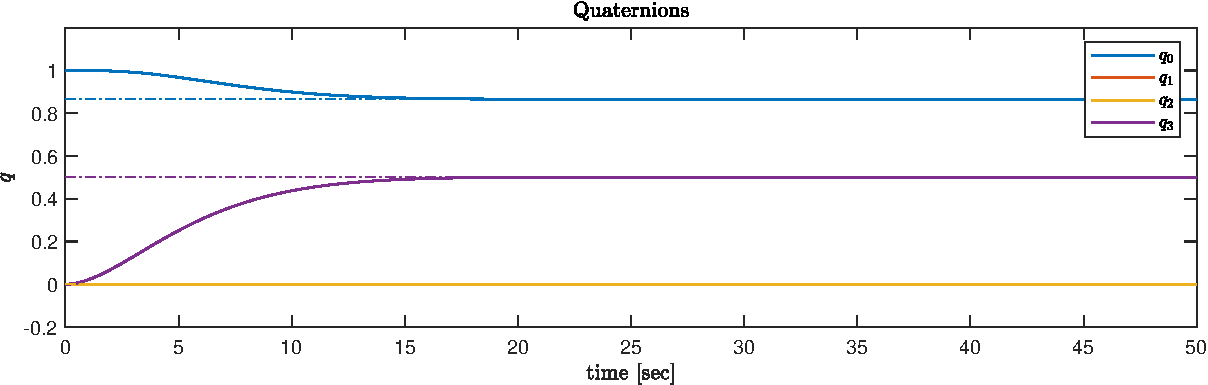
\includegraphics[width=1.0\columnwidth]{figures/plots/RW/rw_rr_y60_q.pdf}
    \caption{Quaternions for RW only rest to rest maneuver}
    \label{plt:rw_rr_y60_q_1}
\end{figure}
\noindent \autoref{plt:rw_rr_y60_q_1} to \autoref{plt:rw_rr_y60_Om_dot_1} are results
for given conditions in \autoref{tbl:states_rw_rr_y60}. It is clear from \autoref{plt:rw_rr_y60_q_1} that system approaches steady state within 20 seconds. Controller gains are selected such that attitude in terms of Euler angle is shown in \autoref{plt:rw_rr_y60_ypr_1} approaches reference yaw angle without overshoot.
\begin{figure}[H]
    \centering
    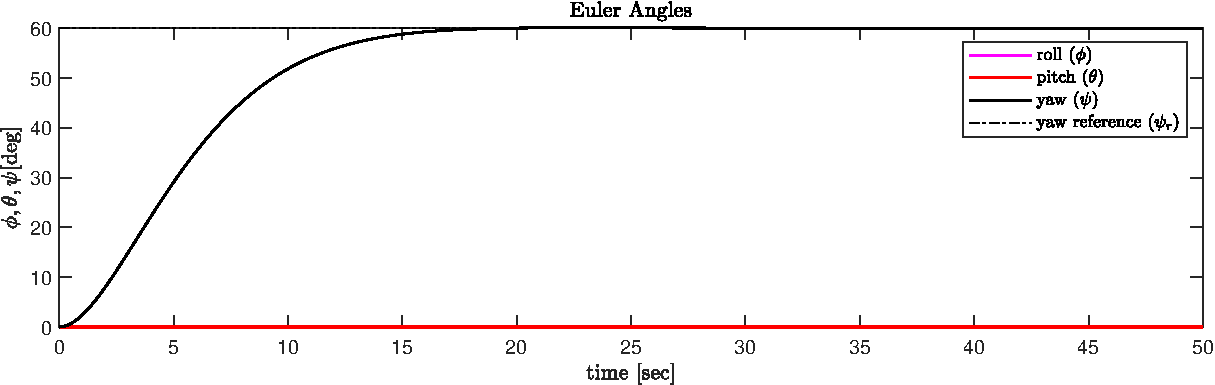
\includegraphics[width=0.9\columnwidth]{figures/plots/RW/rw_rr_y60_ypr.pdf}
    \caption{Euler angles for RW only rest to rest maneuver}
    \label{plt:rw_rr_y60_ypr_1}
\end{figure}

\begin{figure}[H]
    \centering
    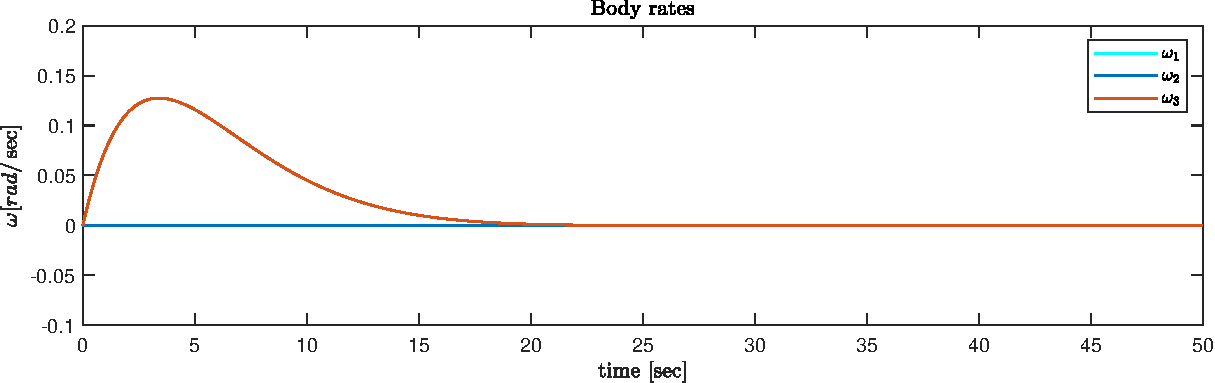
\includegraphics[width=0.9\columnwidth]{figures/plots/RW/rw_rr_y60_w.pdf}
    \caption{Body rates for RW only rest to rest maneuver}
    \label{plt:rw_rr_y60_w_1}
\end{figure}

\noindent Notice in \autoref{plt:rw_rr_y60_w_1} body angular velocity about yaw third axis considered as yaw starts from $0 rad/\sec$. Peak angular velocity $0.125 rad/\sec \approx 7.16^\circ/\sec$ occurs near 4 seconds and overall satisfying agility criteria of $3^\circ/\sec$ by reaching steady state close to $20 \sec$.

\begin{figure}[H]
    \centering
    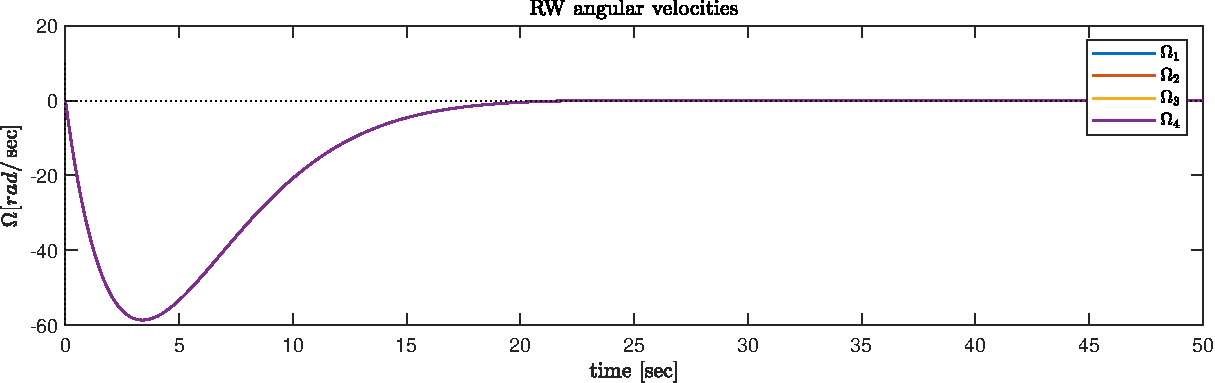
\includegraphics[width=0.9\columnwidth]{figures/plots/RW/rw_rr_y60_Om.pdf}
    \caption{RW velocity for RW only rest to rest maneuver}
    \label{plt:rw_rr_y60_Om_1}
\end{figure}

\begin{figure}[H]
    \centering
    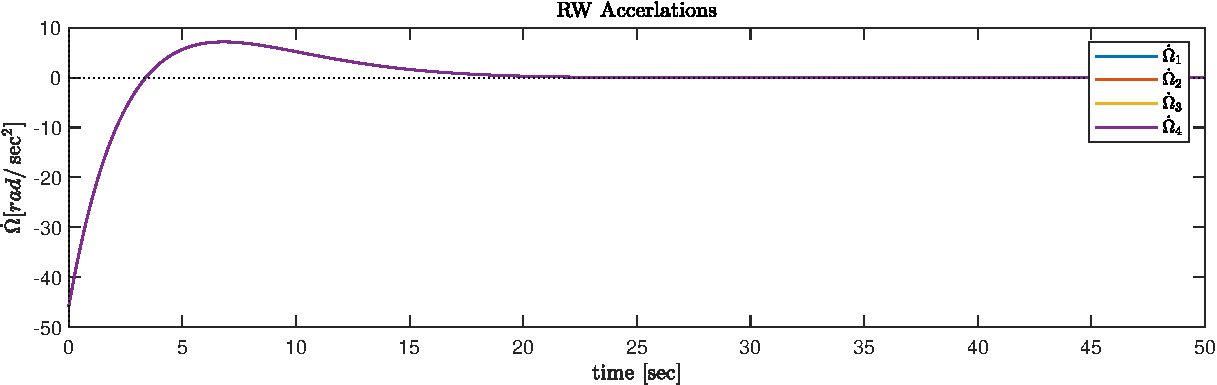
\includegraphics[width=0.8\columnwidth]{figures/plots/RW/rw_rr_y60_Om_dot.pdf}
    \caption{RW accelerations for RW only rest to rest maneuver}
    \label{plt:rw_rr_y60_Om_dot_1}
\end{figure}

\noindent All the reaction wheels rotated in same direction with almost equal rate which is understandable for given situation, maximum wheel speed is within reasonable range close to $60 rad/\sec \approx 570 RPM$, although initial RW acceleration starts from $-50 rad/\sec^2$ which probably should be smoothed by introducing proper gain scheduling, although these results are with preliminary assumption of geometrical properties and inertia and may change for final geometry.


\subsection{Regulation maneuver with RW only ACS}
Consider a scenario in which a satellite with configuration mentioned in \autoref{tbl:sys_param_pre} but subjected to small disturbance along body axis undergoes initial body rate error $\displaystyle \omega _{e} =[ -2\ 5\ 2]^{T} deg/sec$ \ has to counteract this error and should maintain its steady state such a way that asymptotic $\displaystyle q_{e} =[ 1\ 0\ 0\ 0]^{T}$. This is type of station attitude keeping maneuver often needs to performed when satellite deploy it's antenna or solar panel or subjected to impulse disturbance. Starting with same initial conditions from \autoref{tbl:states_rw_rr_y60} except $\displaystyle q_{d} =q=[ 1\ 0\ 0\ 0]^{T}$

\begin{figure}[H]
     \centering
    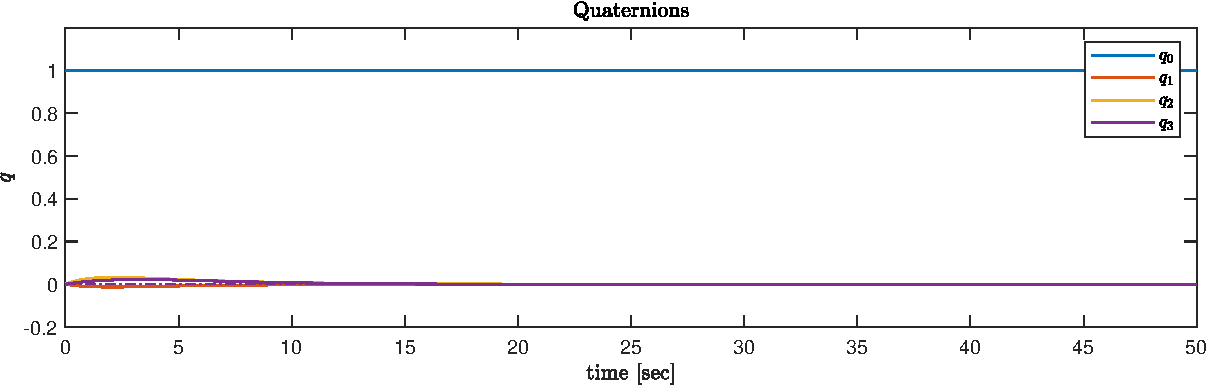
\includegraphics[width=0.8\columnwidth]{figures/plots/RW/rw_reg_w252_q.pdf}
    \caption{Quaternions for RW only station keeping maneuver}
    \label{plt:rw_reg_w252_q_1}
\end{figure}


\begin{figure}[H]
    \centering
    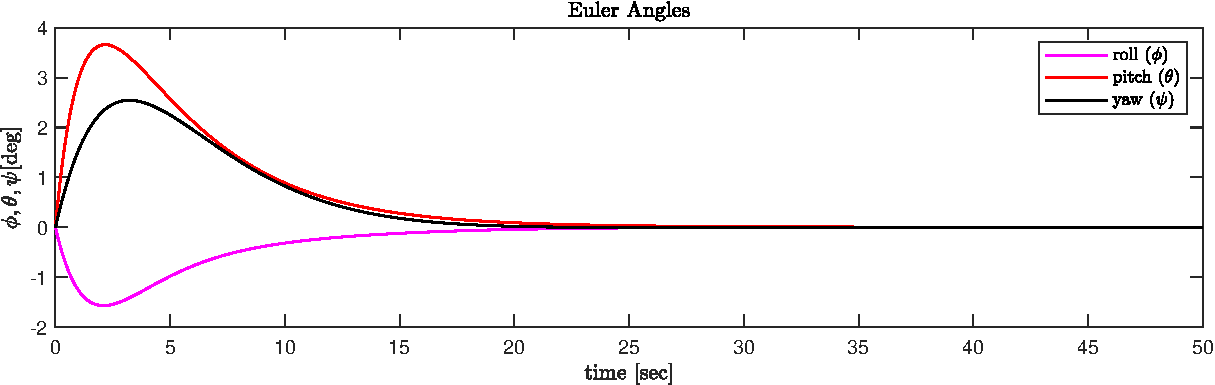
\includegraphics[width=0.8\columnwidth]{figures/plots/RW/rw_reg_w252_ypr.pdf}
    \caption{Euler angles for RW only station keeping maneuver}
    \label{plt:rw_rr_reg_w252_ypr_1}
\end{figure}
\noindent Results of initial body error problem are shown in \autoref{plt:rw_reg_w252_q_1} to  \autoref{plt:rw_rw_reg_w252_Om_dot_1}. We can note quaternion initially at rest are subjected to small variation and approaches its initial state in about 15 seconds. This is clearly visible in terms of Euler angles shown in \autoref{plt:rw_rr_reg_w252_ypr_1} all three angles roll pitch and yaw moved to peak angles approximately $ -1.5\degree, 3.5\degree $ and $ 2.4\degree $ respectively and slowly approaches to zero. Body rates shown in \autoref{plt:rw_reg_w252_w_1} starts from $ [-0.0349, 0.0873 0.0349] rad/sec$ smoothly approaches zero without showing any overshoot thanks to selected controller gain values. 

\begin{equation}
\mathbf{Kq} =\begin{pmatrix}
300 & 0 & 0\\
0 & 300 & 0\\
0 & 0 & 300
\end{pmatrix} ;\quad \mathbf{Kw} =\begin{pmatrix}
850 & 0 & 0\\
0 & 850 & 0\\
0 & 0 & 850
\end{pmatrix}
\label{eqn:RWO_gains}
\end{equation}

\noindent In \autoref{plt:rw_reg_w252_Om_1} notice how RW rates starting from zero diverge initially for 5 seconds and then maintain steady state velocities within range of -50 to 100 rad/sec although these are within the limit but may undergo saturation for large disturbances

\begin{figure}[H]
    \centering
    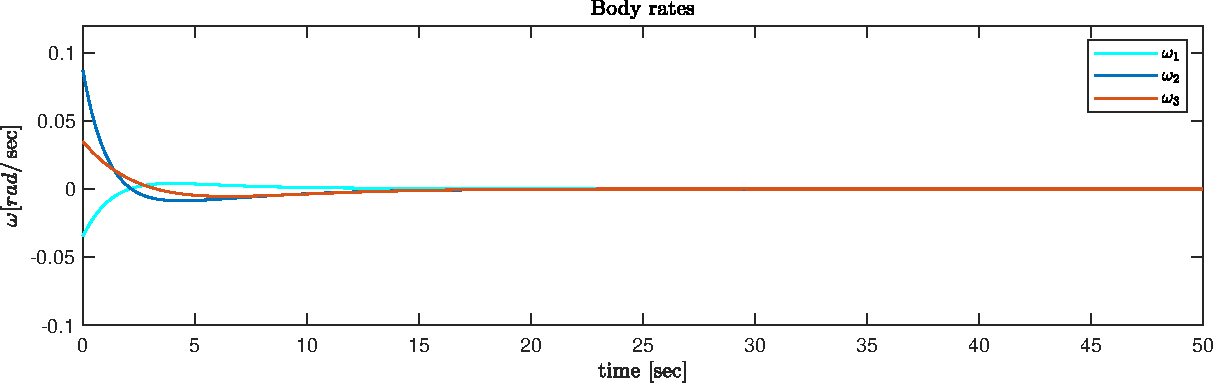
\includegraphics[width=0.9\columnwidth]{figures/plots/RW/rw_reg_w252_w.pdf}
    \caption{Body rates for RW only station keeping maneuver}
    \label{plt:rw_reg_w252_w_1}
\end{figure}


\begin{figure}[H]
    \centering
    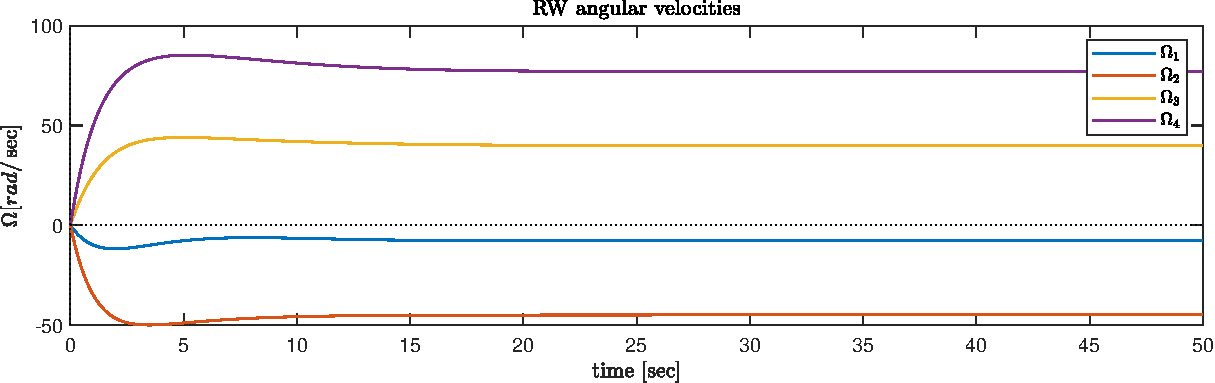
\includegraphics[width=0.9\columnwidth]{figures/plots/RW/rw_reg_w252_Om.pdf}
    \caption{RW velocity for RW only station keeping maneuver}
    \label{plt:rw_reg_w252_Om_1}
\end{figure}

\begin{figure}[H]
    \centering
    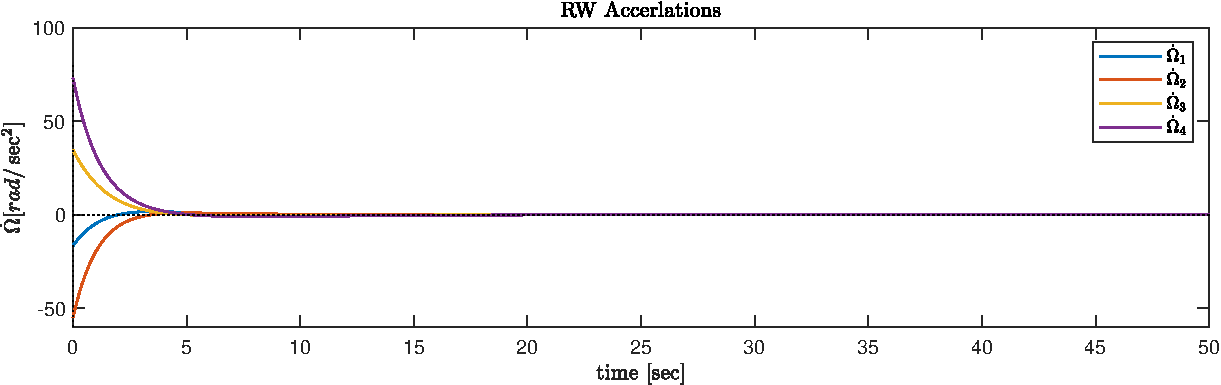
\includegraphics[width=0.9\columnwidth]{figures/plots/RW/rw_reg_w252_Om_dot.pdf}
    \caption{RW accelerations for RW only station keeping maneuver}
    \label{plt:rw_rw_reg_w252_Om_dot_1}
\end{figure}
\noindent From \autoref{plt:rw_rr_y60_Om_dot_1} we can see that Reaction wheels undergoes accelerations with magnitude up to $rad /\sec^2$ this parameter depends on inertia ratio of Platform to RW and can be reduced by either reducing platform inertia or by increasing RW inertia which is not suitable most of the time, thus torque amplification by CMG can be performed.
\section{CMG based ACS}
Despite the fact that RW based ACS is capable of eliminating attitude error in any direction, magnitude of torque produced is very low and limited by RW inertia, and may lead to saturation for large torque requirements. Subsequently, in the interest of taking advantage of torque amplification rest to rest and regulation maneuver are studied with CMG only control system.  
\subsection{Rest to rest reorientation with CMG only ACS}
Consider a satellite has to perform reorientation maneuver in order to cancel the attitude error in Euler angle $[\phi \ \theta \ \psi] = [30 \ 60 \ 90] \deg$ considering initial and desired states mentioned in \autoref{tbl:rr_ypr306090}


\begin{table}[!h]
        \centering
        
\begin{tabular}{p{0.15\textwidth}|p{0.40\textwidth}|p{0.15\textwidth}}
\toprule
 Parameter & Value & Unit \\
\midrule
 $\displaystyle q$ & $\displaystyle [ 1\ 0\ 0\ 0]^{T}$ & - \\
\hline 
 $\displaystyle \omega $ & $\displaystyle [ 0\ 0\ 0]^{T}$ & $\displaystyle \deg /\sec$ \\
\hline 
 $\displaystyle q_{d}$ & $\displaystyle [ 0.6830\ -0.1830\ 0.5000\ 0.5000]^{T}$ & - \\
\hline 
 $\displaystyle \omega _{d}$ & $\displaystyle [ 0\ 0\ 0]^{T}$ & $\displaystyle rad/\sec$ \\
\hline 
 $\displaystyle \delta $ & $\displaystyle \left[\frac{\pi }{2} ,\ \frac{\pi }{2} ,\ \frac{\pi }{2} ,\ \frac{\pi }{2}\right]^{T}$ & $\displaystyle rad$ \\
\hline 
 $\displaystyle \Omega $ & $\displaystyle [ 800,\ 800,\ 800,\ 800]^{T}$ & $\displaystyle rad/\sec$ \\
 \bottomrule
\end{tabular}
        \caption{Initial and desired states for attitude error $\displaystyle \phi =30\degree ,\theta =60\degree ,\ \psi =90\degree $}
\label{tbl:rr_ypr306090}
\end{table}
\noindent Time criterion for maneuver to be performed within 30 seconds will demonstrate performance beyond baseline agility requirement, and to do so Horowitz gains should be carefully selected for asymptotic stability. 


\begin{equation}
\mathbf{Kq} =\begin{pmatrix}
1 & 0 & 0\\
0 & 1 & 0\\
0 & 0 & 1
\end{pmatrix} ;\quad \mathbf{Kw} =\begin{pmatrix}
1.5 & 0 & 0\\
0 & 1.5 & 0\\
0 & 0 & 1.5
\end{pmatrix}
\label{eqn:CMO_gains}
\end{equation}
Notice gains selected for \acrshort{cmg} only \acrshort{acs} are much lower than those mentioned in \autoref{eqn:RWO_gains} selected for \acrshort{rw}  only \acrshort{acs}, we can infer that CMG can produce much higher torques compared with RW thus gain is reduced by order of magnitude of hundreds.

\begin{figure}[H]
     \centering
    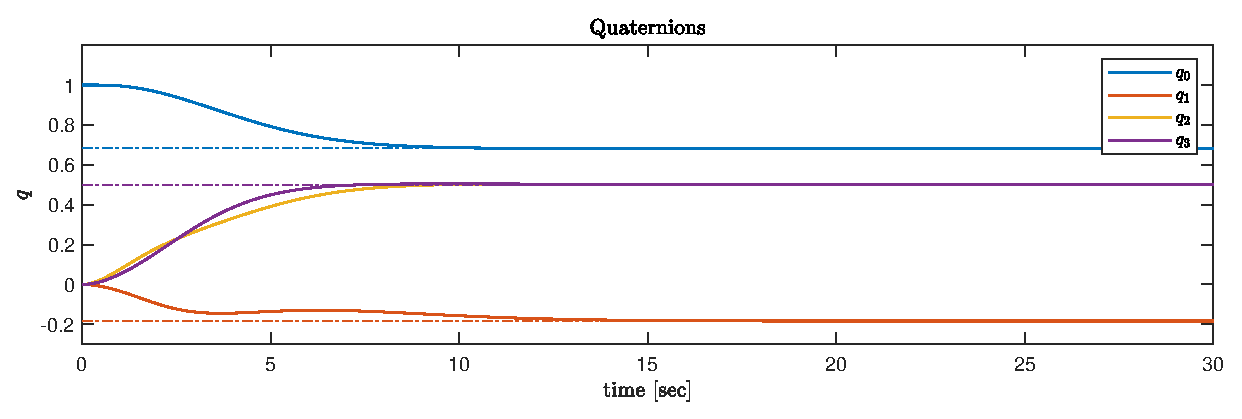
\includegraphics[width=0.9\columnwidth]{figures/plots/CMG/cm_rr_ypr369_q.eps}
    \caption{Quaternions for CMG only reorientation with attitude error $\displaystyle [\phi\ \theta\ \psi] =[30,\ 60,\ 90]\degree $}
    \label{plt:cm_rr_ypr369_q_2}
\end{figure}

\begin{figure}[H]
     \centering
    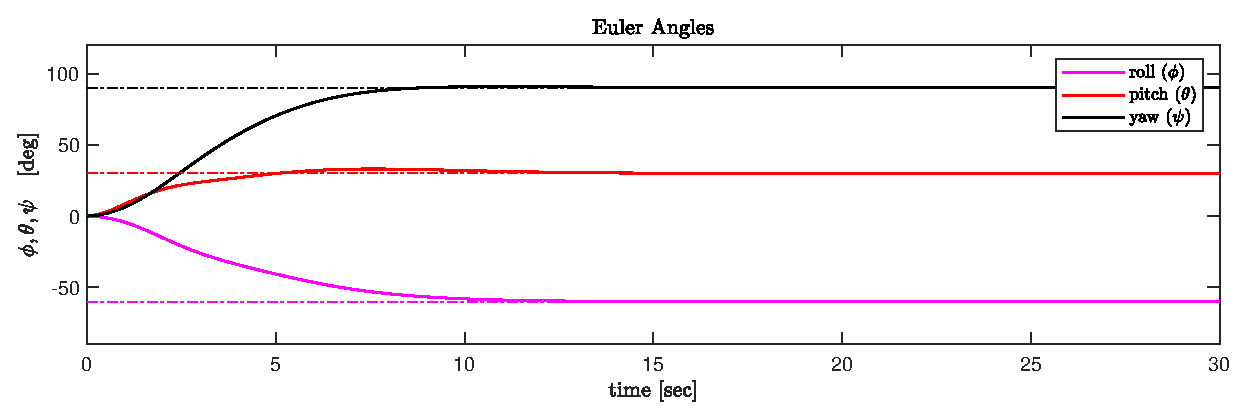
\includegraphics[width=0.9\columnwidth]{figures/plots/CMG/cm_rr_ypr369_ypr.eps}
    \caption{Euler angles for CMG only reorientation with attitude error $\displaystyle [\phi\ \theta\ \psi] =[30,\ 60,\ 90]\degree $}
    \label{plt:cm_rr_ypr369_ypr_2}
\end{figure}
\autoref{plt:cm_rr_ypr369_q_2} to \autoref{plt:cm_rr_ypr369_delta_dot_dot_2} are results for attitude error compensation maneuver with reference roll pitch yaw set as $\displaystyle [\phi\ \theta\ \psi] =[30,\ 60,\ 90]\degree $. Since gimbal state is far away from singularity, satellite smoothly approaches to reference states clearly seen from \autoref{plt:cm_rr_ypr369_q_2} and \autoref{plt:cm_rr_ypr369_ypr_2}.
\begin{figure}[H]
     \centering
    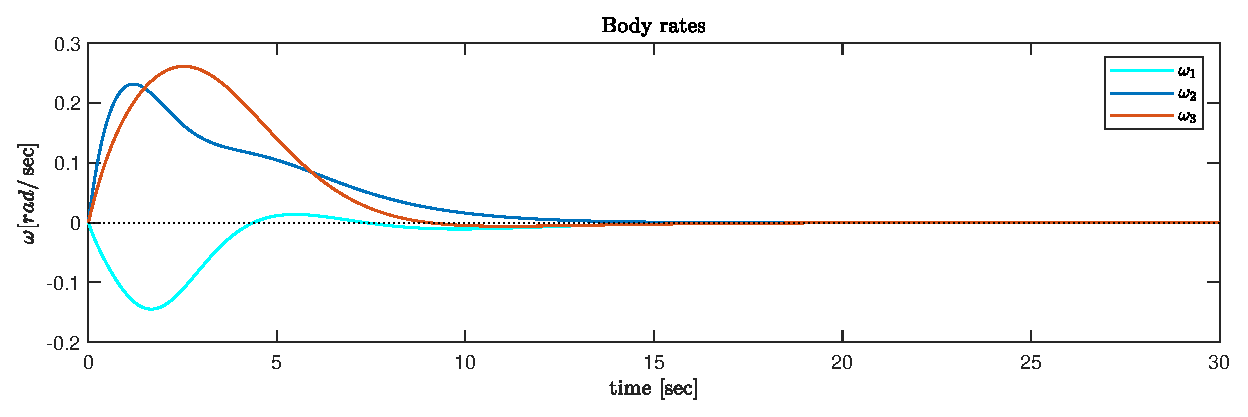
\includegraphics[width=0.9\columnwidth]{figures/plots/CMG/cm_rr_ypr369_w.eps}
    \caption{Body rates for CMG only reorientation with attitude error $\displaystyle [\phi\ \theta\ \psi] =[30,\ 60,\ 90]\degree $}
    \label{plt:cm_rr_ypr369_w_2}
\end{figure}
With negligible overshoot in body rate about third axis, satellite reaches steady state within 20 seconds seen in \autoref{plt:cm_rr_ypr369_w_2}. Gimbal angles initially set at $\pi/2 rad$ remains within magnitude of 1.2 to 1.9 radiance and no more than $20 \degree$ variation in gimbal angles is noticeable in \autoref{plt:cm_rr_ypr369_delta_2}. Although gimbal angular velocities shown in \autoref{plt:cm_rr_ypr369_delta_dot_2} has rapid variations which is understandable due to such a large slew motion is performed within 20 seconds.Moreover, smooth curves denotes CMG, was far away from singularity. 

\begin{figure}[H]
     \centering
    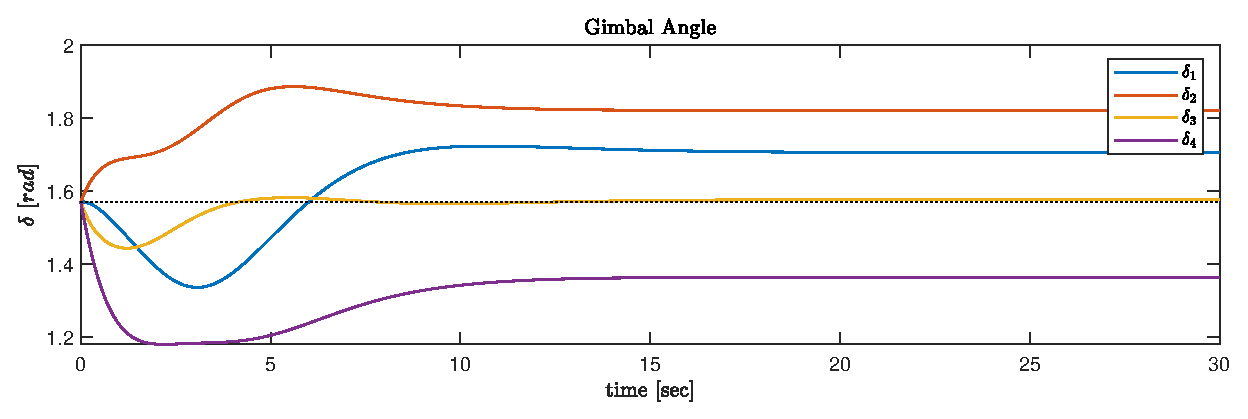
\includegraphics[width=0.9\columnwidth]{figures/plots/CMG/cm_rr_ypr369_delta.eps}
    \caption{Gimbal angles for CMG only reorientation with attitude error $\displaystyle [\phi\ \theta\ \psi] =[30,\ 60,\ 90]\degree $}
    \label{plt:cm_rr_ypr369_delta_2}
\end{figure}

\begin{figure}[H]
     \centering
    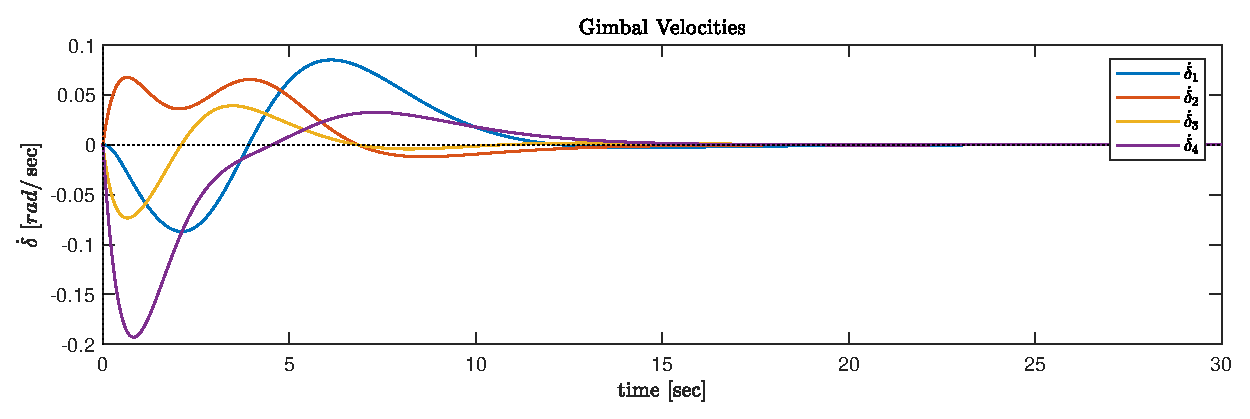
\includegraphics[width=0.9\columnwidth]{figures/plots/CMG/cm_rr_ypr369_delta_dot.eps}
    \caption{Gimbal rates for CMG only reorientation with attitude error $\displaystyle [\phi\ \theta\ \psi] =[30,\ 60,\ 90]\degree $}
    \label{plt:cm_rr_ypr369_delta_dot_2}
\end{figure}
\noindent Gimbal acceleration shown in \autoref{plt:cm_rr_ypr369_delta_dot_dot_2} are signals provided to gimbal motor in order to track required gimbal velocity for steering law. These accelerations are proportional to current supplied to gimbal motor. Acceleration magnitude is within range of $1 rad/\sec^2$ will not compromise the structural integrity of system.

\begin{figure}[H]
     \centering
    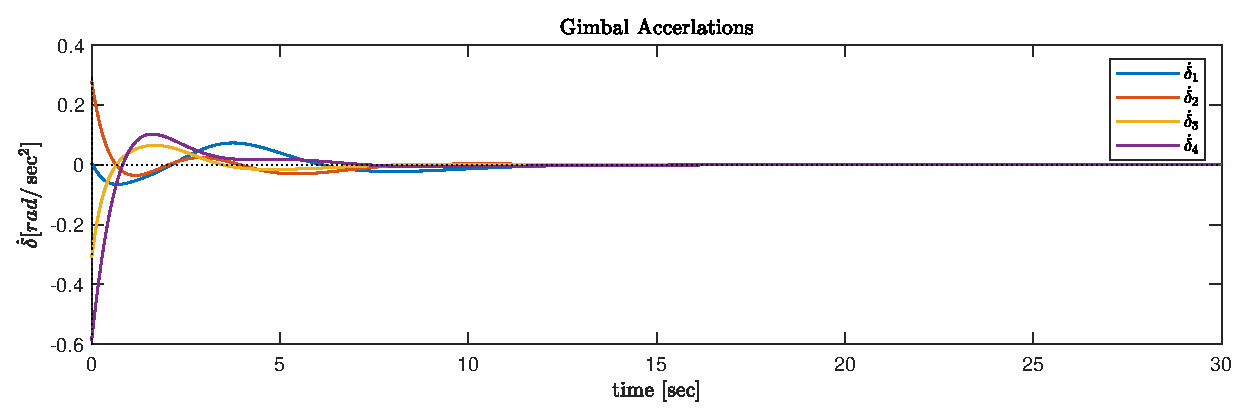
\includegraphics[width=0.9\columnwidth]{figures/plots/CMG/cm_rr_ypr369_delta_dot_dot.eps}
    \caption{Gimbal rates for CMG only reorientation with attitude error $\displaystyle [\phi\ \theta\ \psi] =[30,\ 60,\ 90]\degree $}
    \label{plt:cm_rr_ypr369_delta_dot_dot_2}
\end{figure}

\subsection{Body rate regulation with CMG only ACS}
Consider another scenario in which satellite is subjected to  step disturbance, ACS has to cancel angular velocity error and approach to its initial attitude, considering states from 


\begin{table}[!h]
        \centering
        
\begin{tabular}{p{0.15\textwidth}|p{0.40\textwidth}|p{0.15\textwidth}}
\toprule
 Parameter & Value & Unit \\
\midrule
 $\displaystyle q=q_{d}$ & $\displaystyle [ 1\ 0\ 0\ 0]^{T}$ & - \\
\hline 
 $\displaystyle \omega $ & $\displaystyle [ 0\ 10\ 0]^{T}$ & $\displaystyle \deg /\sec$ \\
\hline 
 $\displaystyle \omega _{d}$ & $\displaystyle [ 0\ 0\ 0]^{T}$ & $\displaystyle rad/\sec$ \\
\hline 
 $\displaystyle \delta $ & $\displaystyle [ 0,\ 0,\ 0,0]^{T}$ & $\displaystyle rad$ \\
\hline 
 $\displaystyle \Omega $ & $\displaystyle [ 800,\ 800,\ 800,\ 800]^{T}$ & $\displaystyle rad/\sec$ \\
 \bottomrule
\end{tabular}
\caption{Initial and desired states for angular velocity error with CMG in singular configuration}
\label{tbl_cmg_at_sing}
\end{table}
It is clear that CMG is at inescapable singularity thus combination of SVD bassed and off diagonal singularity avoidance steering law is used with gains selected by trial and error with numerous iterations.

\begin{equation}
\mathbf{Kq} =\begin{pmatrix}
5.3 & 0 & 0\\
0 & 5.3 & 0\\
0 & 0 & 5.3
\end{pmatrix} ;\quad \mathbf{Kw} =\begin{pmatrix}
2.5 & 0 & 0\\
0 & 2.5 & 0\\
0 & 0 & 2.5
\end{pmatrix}
\end{equation}
with using off diagonal singularity robust steering steering law as
\begin{equation}
\dot{\delta } =\mathbf{W}\mathcal{G}^{T}_{t}\left(\mathcal{G}_{t}\mathbf{W}\mathcal{G}^{T}_{t} +\lambda \mathbf{E}\right)^{-1} +\lambda \mathbf{v}_{1}
\end{equation}
where, weight matrices are selected by adding off diagonal harmonics as
\begin{equation*}
\mathbf{W} =\begin{pmatrix}
1 & \lambda  & \lambda  & \lambda \\
\lambda  & 2 & \lambda  & \lambda \\
\lambda  & \lambda  & 3 & \lambda \\
\lambda  & \lambda  & \lambda  & 4
\end{pmatrix}
\end{equation*}and
\begin{equation*}
\mathbf{E} =\begin{pmatrix}
100 & \epsilon _{3} & \epsilon _{2}\\
\epsilon _{3} & 100 & \epsilon _{1}\\
\epsilon _{2} & \epsilon _{1} & 100
\end{pmatrix}
\end{equation*}
with $ \epsilon _{i} =0.1\sin( \pi t+\varphi ) ,\ \varphi _{i} =\{0,\pi /2,\pi \}$ and $ \lambda =0.1\exp\left( -10\det\left(\mathcal{G}_{t}\mathcal{G}^{T}_{t}\right)\right)$ 
Results of CMG at singular states are shown in simulation \autoref{plt:cm_reg_w10_q} to \autoref{plt:zoom_plots_omega_sing}. Since CMG singularity is zero at the beginning satellite slowly diverges from set point, at first it performs complete $360 \degree$ rotation in yaw axis for about 245 seconds shown in \autoref{plt:cm_reg_w10_ypr}. Note that even there is discontinuity visible at 150 seconds, it is due to wrapping of Euler angles within range of -180$\degree$ to 180$\degree$ Rapid variation in body rate occurs, a spike seen near $250$ seconds in \autoref{plt:cm_reg_w10_w} and from zoomed view of body rate shown in \autoref{plt:cm_reg_w10_zoom_w} magnitude of about $1.5 rad/\sec$ occurs before reaching steady within next 10 seconds.
\begin{figure}[H]
     \centering
    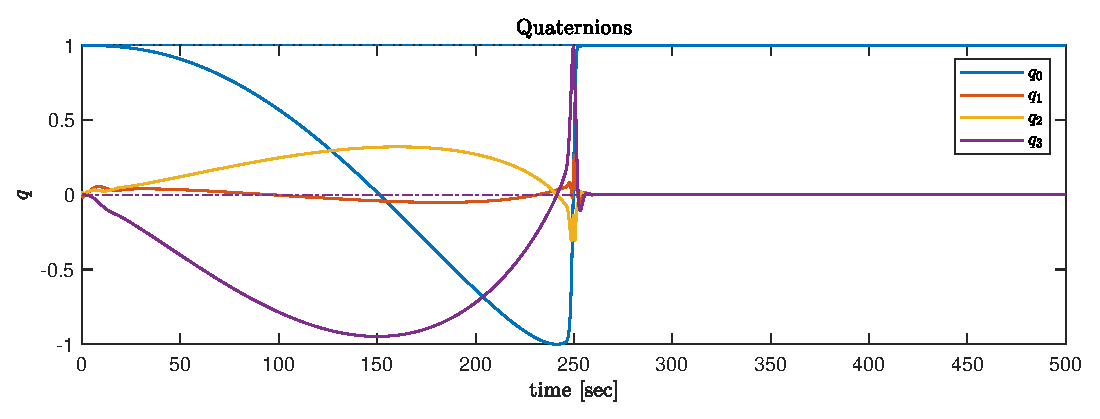
\includegraphics[width=0.9\columnwidth]{figures/plots/CMG/cm_reg_w10_q.eps}
    \caption{Quaternions for station keeping with CMG only ACS}
    \label{plt:cm_reg_w10_q}
\end{figure}

\begin{figure}[H]
     \centering
    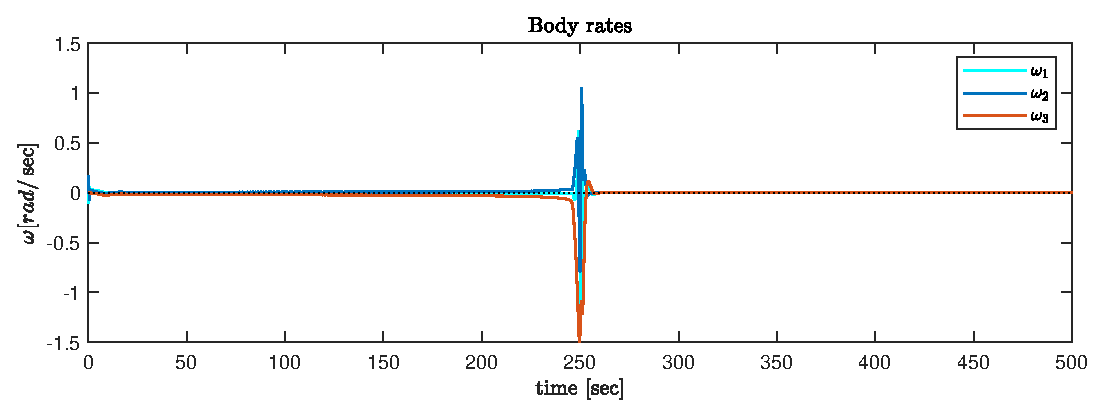
\includegraphics[width=0.9\columnwidth]{figures/plots/CMG/cm_reg_w10_w.eps}
    \caption{Body Rates for station keeping with CMG only ACS}
    \label{plt:cm_reg_w10_w}
\end{figure}



\begin{figure}[H]
     \centering
    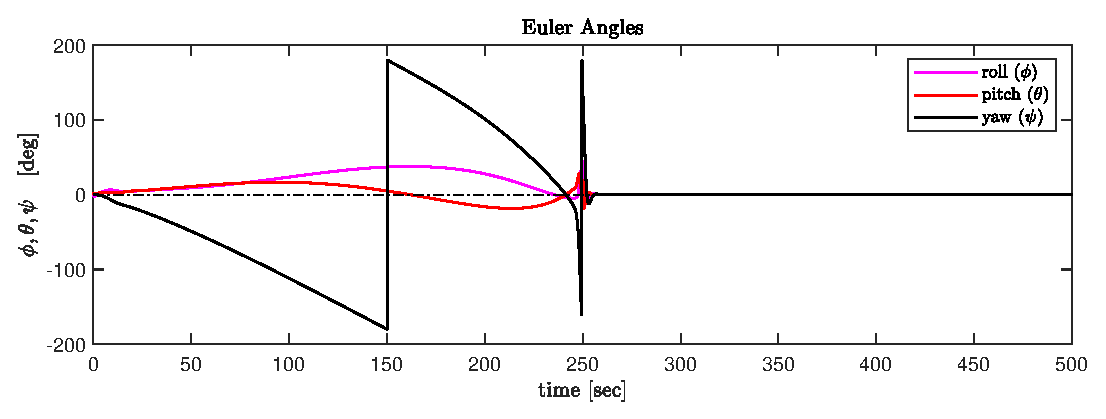
\includegraphics[width=0.9\columnwidth]{figures/plots/CMG/cm_reg_w10_ypr.eps}
    \caption{Euler angles for station keeping with CMG only ACS}
    \label{plt:cm_reg_w10_ypr}
\end{figure}
\noindent Gimbal angles slowly increase till 240 seconds and sudden jump occurs near 250 seconds. \autoref{plt:cm_reg_w10_delta_dot} and \autoref{plt:cm_reg_w10_zoom_delta_dot} are gimbal velocity and its zoomed view, notice how gimbal velocities rapidly change from 245 to 255 seconds Despite the fact that gimbal velocities are not exceptionally high, entire maneuver took about 270 seconds before reaching steady state which is not favorable. Thus being capable of producing large torque amplification, CMG alone can not guarantee smooth tracking performance. Moreover, finding perfect parameters and gains for particular task is not trivial since they vary depending on type of singularity and state.
\begin{figure}[H]
     \centering
    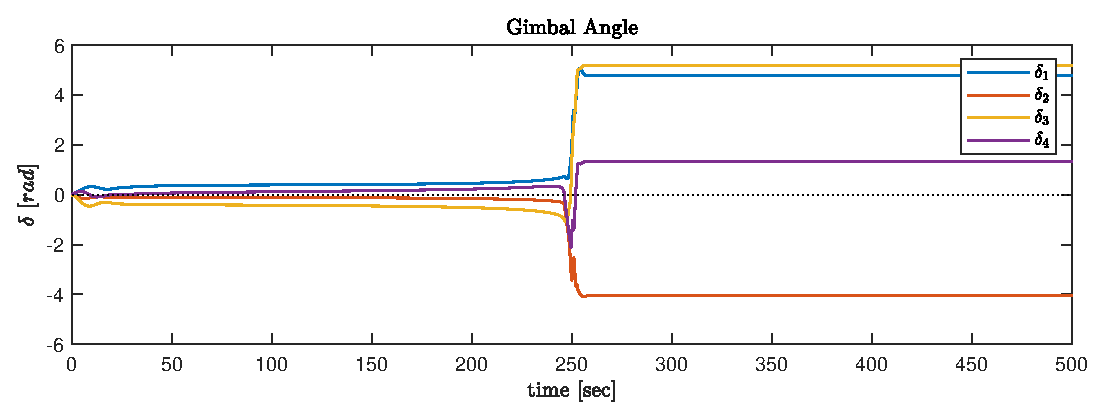
\includegraphics[width=0.9\columnwidth]{figures/plots/CMG/cm_reg_w10_delta.eps}
    \caption{Gimbal angles for station keeping with CMG only ACS}
    \label{plt:cm_reg_w10_delta}
\end{figure}

\begin{figure}[H]
     \centering
    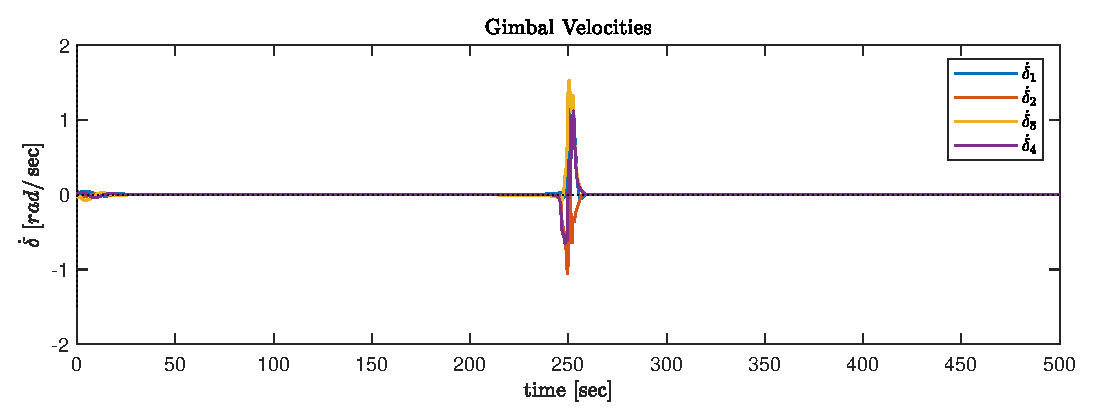
\includegraphics[width=0.9\columnwidth]{figures/plots/CMG/cm_reg_w10_delta_dot.eps}
    \caption{Gimbal velocities for station keeping with CMG only ACS}
    \label{plt:cm_reg_w10_delta_dot}
\end{figure}

\begin{figure}[H]
    \centering
  \begin{subfigure}[b]{0.49\columnwidth}
     \centering
    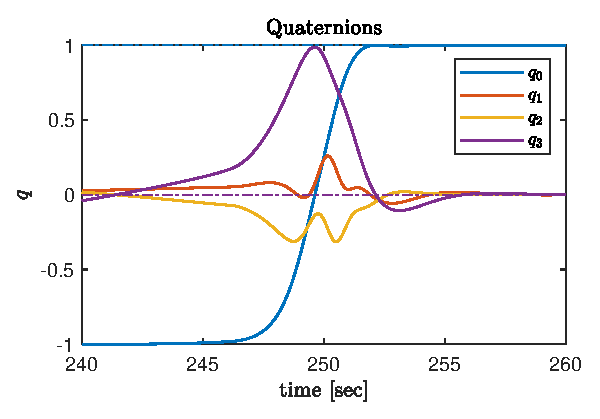
\includegraphics[width=1\columnwidth]{figures/plots/CMG/cm_reg_w10_zoom_q.eps}
    \caption{Quaternions}
    \label{plt:cm_reg_w10_zoom_q}
\end{subfigure}
  %
  \begin{subfigure}[b]{0.49\columnwidth}
     \centering
    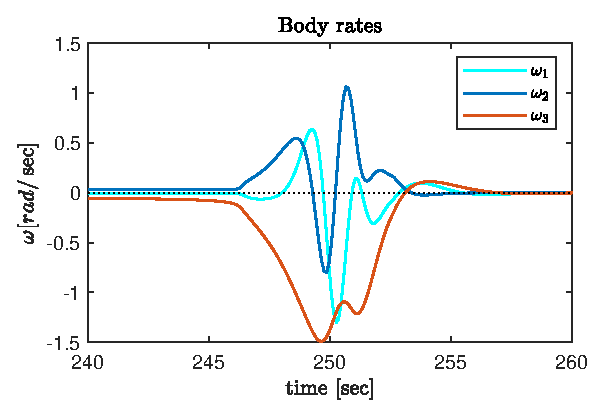
\includegraphics[width=1\columnwidth]{figures/plots/CMG/cm_reg_w10_zoom_w.eps}
    \caption{Body Rates}
    \label{plt:cm_reg_w10_zoom_w}
\end{subfigure}
  %
  \begin{subfigure}[b]{0.49\columnwidth}
     \centering
    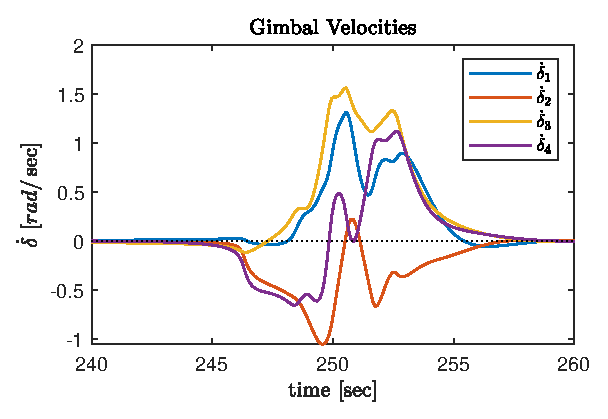
\includegraphics[width=1\columnwidth]{figures/plots/CMG/cm_reg_w10_zoom_delta_dot.eps}
    \caption{Gimbal velocities}
    \label{plt:cm_reg_w10_zoom_delta_dot}
\end{subfigure}
  %
  \begin{subfigure}[b]{0.49\columnwidth}
     \centering
    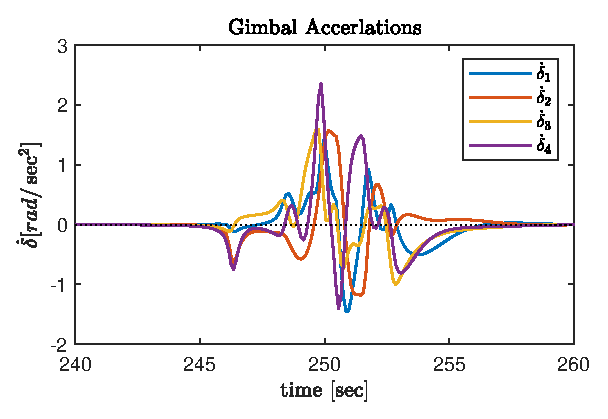
\includegraphics[width=1\columnwidth]{figures/plots/CMG/cm_reg_w10_zoom_delta_dot_dot.eps}
    \caption{Gimbal accerlations}
    \label{plt:cm_reg_w10_zoom_delta_dot_dot}
\end{subfigure}
\caption{Zoomed view of station keeping maneuver with CMG only ACS}
\label{plt:zoom_plots_omega_sing}

\end{figure}

\section{VSCMG based ACS}
In this section simulation results \acrlong{acs} based of complete \acrlong{vscmg} arranged in as pyramid cluster is discussed. Two types of simulations are performed first comparison with only CMG based ACS and later trajectory tracking maneuver is presented.

\section{Body rate regulation with VSCMG}
Considering same scenario of CMG only ACS discussed in previous section. We have deliberately set the gimbal configuration satellite state and initial angular velocity as shown in \autoref{tbl_cmg_at_sing} so that CMG is in singular state. Now advancing with same situation occurred with VSCMG based ACS. Controller gains and steering parameters are set as

\begin{equation}
\mathbf{Kq} =\begin{pmatrix}
300 & 0 & 0\\
0 & 300 & 0\\
0 & 0 & 300
\end{pmatrix} ;\quad \mathbf{Kw} =\begin{pmatrix}
850 & 0 & 0\\
0 & 850 & 0\\
0 & 0 & 850
\end{pmatrix}
\end{equation}

\noindent Notice selected gains are much higher than CMG only ACS. Bearing in mind that with higher gains were not Horowitz due to singularities present in CMG and bringing settling closer to 60 seconds was not possible. 
\noindent And constants for off-diagonal singularity robust steering law are 

\begin{equation*}
\begin{aligned}
\lambda  & =0.01\exp( -10m_{c})\\
\beta _{i} & =\min\left\{1\times 10^{3}\exp( -0.01m_{c} /m_{v}) ,\ 1000\right\}\\
\kappa  & =0.001\exp( -10m_{v})
\end{aligned}
\end{equation*}
 here $\beta_i $ is clipped to 1000  in order to avoid computational singularity when $m_v$ approaches zero. \begin{figure}[H]
     \centering
    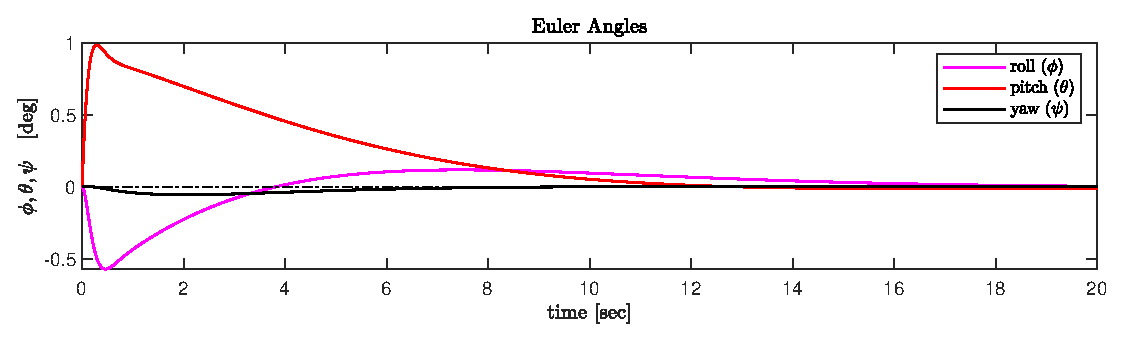
\includegraphics[width=0.9\columnwidth]{figures/plots/VSCMG/vs_reg_w10_ypr.eps}
    \caption{Euler angles for station keeping with VSCMG in vicinity of singularity}
    \label{plt:vs_reg_w10_ypr}
\end{figure}

\begin{figure}[H]
     \centering
    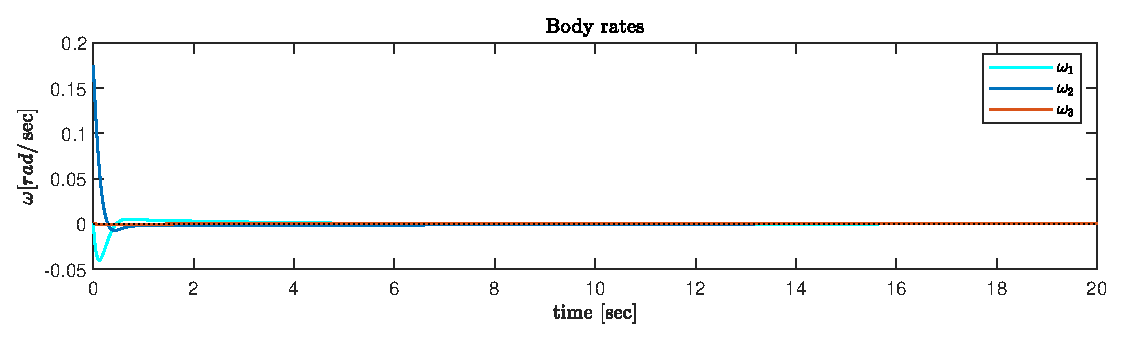
\includegraphics[width=0.9\columnwidth]{figures/plots/VSCMG/vs_reg_w10_w.eps}
    \caption{Body rates for station keeping with VSCMG in vicinity of singularity}
    \label{plt:vs_reg_w10_w}
\end{figure}
\noindent Upon initial disturbance Euler angles first rapidly increase but does not change more than $1 \degree$ due to high value of $ \textbf{K}_w $ and smoothly settles to desired state within 20 seconds as shown in \autoref{plt:vs_reg_w10_ypr}. Cancellation of velocity error verified from body rates shown in \autoref{plt:vs_reg_w10_w}

\begin{figure}[H]
     \centering
    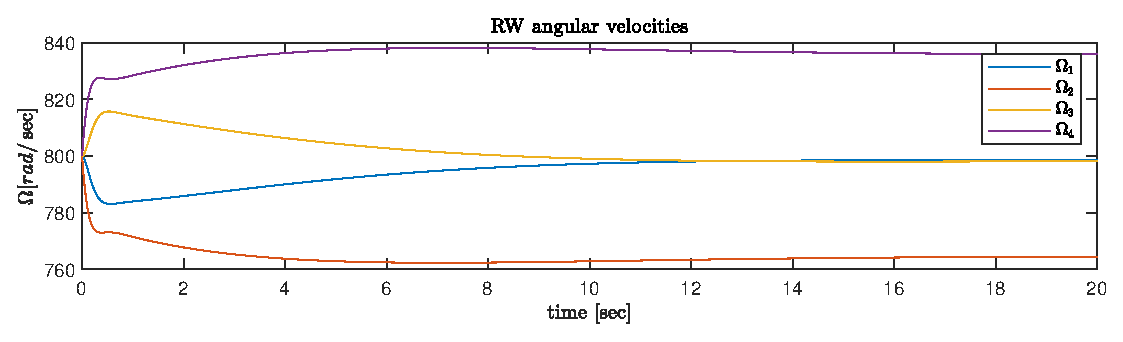
\includegraphics[width=0.9\columnwidth]{figures/plots/VSCMG/vs_reg_w10_Om.eps}
    \caption{RW rates for station keeping with VSCMG in vicinity of singularity}
    \label{plt:vs_reg_w10_Om}
\end{figure}

\begin{figure}[H]
     \centering
    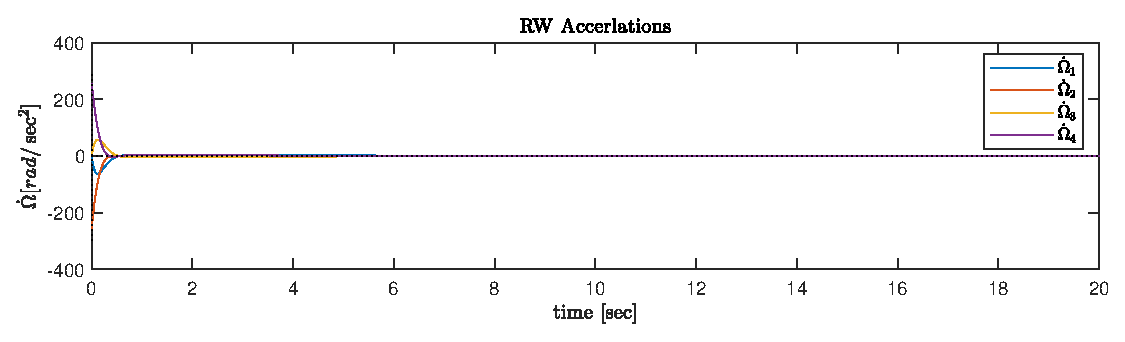
\includegraphics[width=0.9\columnwidth]{figures/plots/VSCMG/vs_reg_w10_Om_dot.eps}
    \caption{RW accelerations for station keeping with VSCMG in vicinity of singularity}
    \label{plt:vs_reg_w10_Om_dot}
\end{figure}
\noindent Despite RW change in velocities in \autoref{plt:vs_reg_w10_Om} are not too large, they are subjected to high accelerations shown in \autoref{plt:vs_reg_w10_Om_dot} with maximum magnitude if  $220\ rad/\sec^2$ which can be minimized with relaxed settling time criterion. At the same time gimbal velocities are considerably low which is evident due to high momentum of RW. Overall there is no chattering or high frequency components present in any of state despite existence of singularity.
\begin{figure}[H]
     \centering
    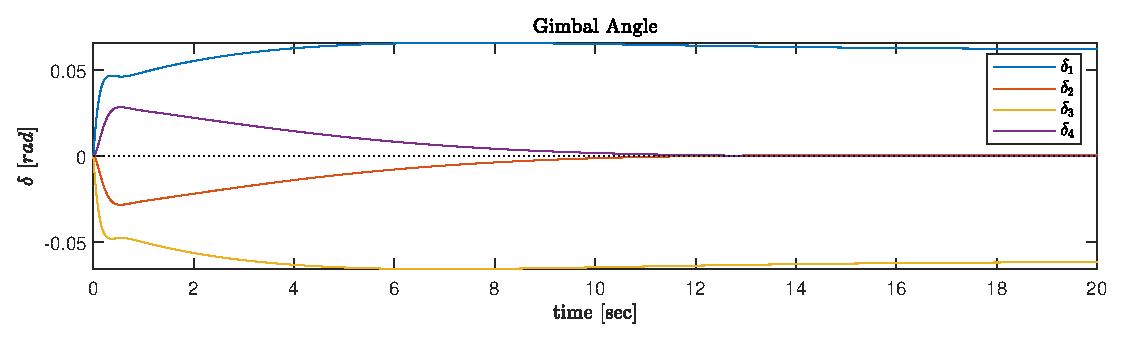
\includegraphics[width=0.9\columnwidth]{figures/plots/VSCMG/vs_reg_w10_delta.eps}
    \caption{Gimbal angles for station keeping with VSCMG in vicinity of singularity}
    \label{plt:vs_reg_w10_delta}
\end{figure}

\begin{figure}[H]
     \centering
    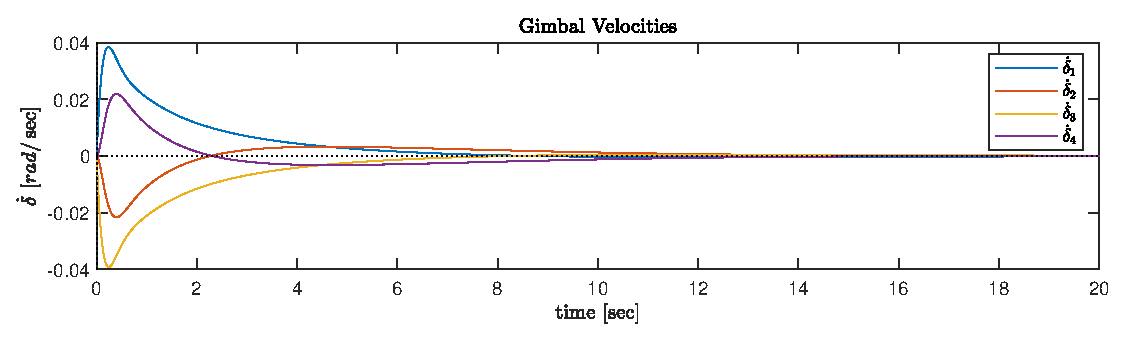
\includegraphics[width=0.9\columnwidth]{figures/plots/VSCMG/vs_reg_w10_delta_dot.eps}
    \caption{Gimbal velocities for station keeping with VSCMG in vicinity of singularity}
    \label{plt:vs_reg_w10_delta_dot}
\end{figure}

\section{Trajectory tracking with VSCMG ACS}
For verification of VSCMG based ACS and in order to test capabilities of steering law for large maneuvers for long period. An hypothetical scenario is assumed as a nadir pointing satellite in highly elliptical orbit has to maintain its payload towards earth. Since for elliptical satellite has to rotate at non constant speed in order to maintain its attitude with respect to true anomaly.
\newacronym{heo}{HEO}{Highly Elliptical Orbit}
Orbital parameters of ``MOLNIYA 1-86'' launched on 26 May 1993 by USSR is taken as reference satellite. A \acrlong{heo} with parameters shown in \autoref{tbl:MOLNIYA_param} was communications satellite used to test  a system of radio communications and television broadcasting using earth satellites as active transponders and to experiment with the system in practical use.\cite{Molniya}
\begin{table}[!h]
\centering
\begin{tabular}{p{0.30\textwidth}|p{0.20\textwidth}|p{0.15\textwidth}}
\toprule
 Parameter & Value & Unit \\
\midrule
 Inclination & 63.103 & $\displaystyle \deg$ \\
\hline 
 Eccentricity & 0.48485 & - \\
\hline 
 Semi major axis & 13353.0 & km \\
\hline 
 Apogee & 13457.1 & km \\
\hline 
 Perigee & 508.0 & km \\
\hline 
 Time period & 15354.2 & sec \\
 \bottomrule
\end{tabular}
\caption{MOLNIYA 1-86 Orbital details}
\label{tbl:MOLNIYA_param}
\end{table}

Reference trajectory in terms of Euler axis angle is realized by numerically solving Kepler equations of mean motion ($n$), Mean ($M$) Eccentric ($E$) and True anomaly
\begin{equation}
n=\sqrt{\frac{\mu }{a^{3}}}
\end{equation}
\begin{equation}
\begin{aligned}
M & =M_{0} +n( t-t_{0})\\
M & =E-e\sin E
\end{aligned}
\end{equation}
\begin{equation}
\tan\frac{\nu }{2} =\sqrt{\frac{1+e}{1-e}}\tan\frac{E}{2}
\end{equation}
Iterative solution is used to find mean anomalies for 10 periods of satellite to form a reference trajectory such that axis orthogonal to orbital plane is rotated by angle $\nu$ and quaternions are competed as

\begin{equation*}
q( t) =\left[\cos\frac{\nu ( t)}{2} ,0,0,\sin\frac{\nu ( t)}{2}\right]^{T}
\end{equation*}
Reference quaternions for Nine complete orbits are shown in \autoref{plt:molnia_ref_tack} and results of trajectory tracking are shown from \autoref{plt:vs_ref_mol_Om} to \autoref{plt:vs_ref_mol_Om}.

\begin{figure}[H]
     \centering
    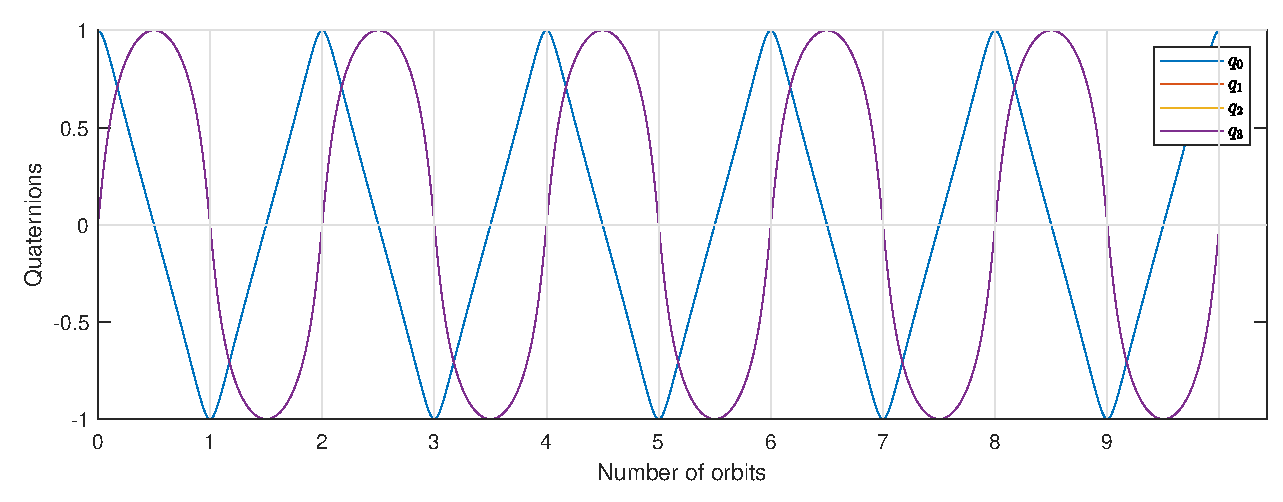
\includegraphics[width=0.9\columnwidth]{figures/plots/VSCMG/molnia_ref_tack.eps}
    \caption{Reference trajectory quaternions computed for MOLNIYA 1-86}
    \label{plt:molnia_ref_tack}
\end{figure}
\noindent Since trajectory tracked by satellite overlaps reference trajectory, least square residuals between reference quaternions and simulated quaternions are shown in \autoref{plt:vs_ref_mol_q_e} notice the deviation is within order of magnitude $10^{-6}$ 
\begin{figure}[H]
     \centering
    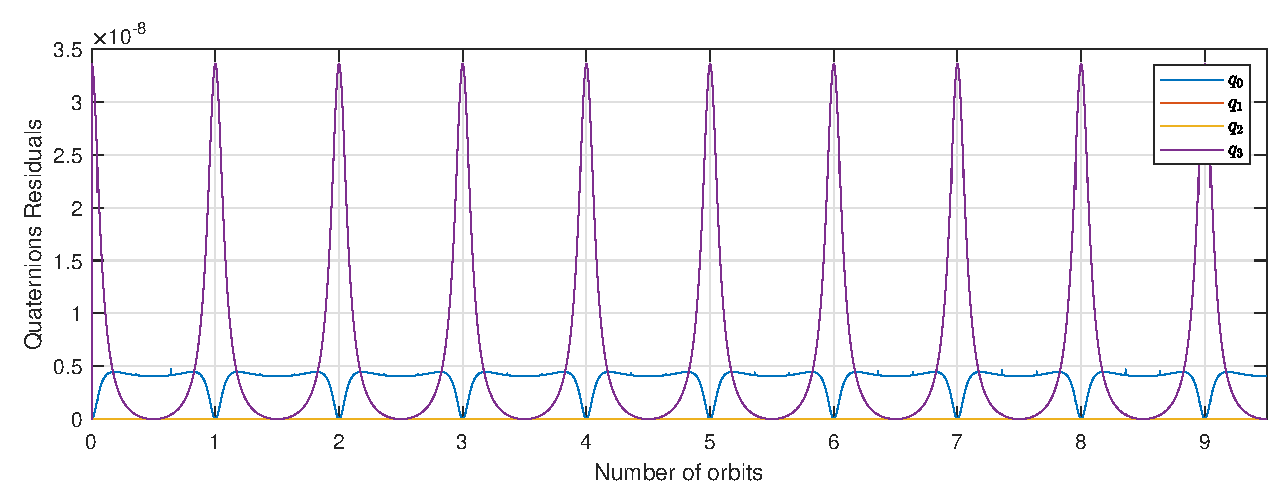
\includegraphics[width=0.9\columnwidth]{figures/plots/VSCMG/vs_ref_mol_q_e.eps}
    \caption{Least square residuals of quaternions computed for MOLNIYA 1-86}
    \label{plt:vs_ref_mol_q_e}
\end{figure}
\noindent Pitch and roll axis were placed in orbital plane, 9 complete revolutions are seen about yaw axis shown in \autoref{plt:vs_ref_mol_ypr}.
\begin{figure}[H]
     \centering
    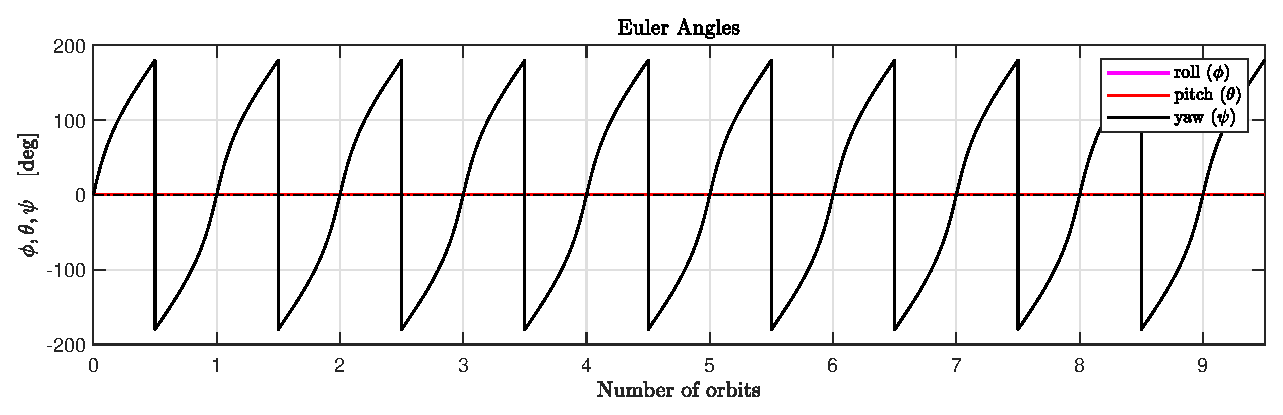
\includegraphics[width=0.9\columnwidth]{figures/plots/VSCMG/vs_ref_mol_ypr.eps}
    \caption{Euler angles computed for MOLNIYA 1-86}
    \label{plt:vs_ref_mol_ypr}
\end{figure}
Satellite orbital period is large and has to perform only one revolution per orbit due as a result body rates of tracked trajectory are very low. Although we can see from peaks at each orbit that rates slows down till apogee and accelerate till perigee.
\begin{figure}[H]
     \centering
    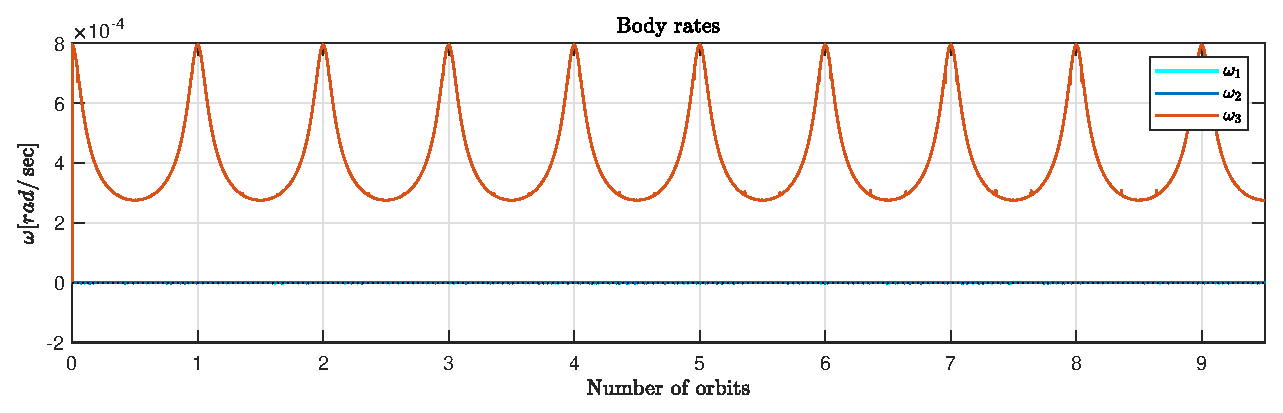
\includegraphics[width=0.9\columnwidth]{figures/plots/VSCMG/vs_ref_mol_w.eps}
    \caption{Body rates for trajectory tracking maneuver}
    \label{plt:vs_ref_mol_w}
\end{figure}
\noindent Similarly, in order to maintain varying body rate, RW velocities oscillate within magnitude of 0.2 $rad/sec$
\begin{figure}[H]
     \centering
    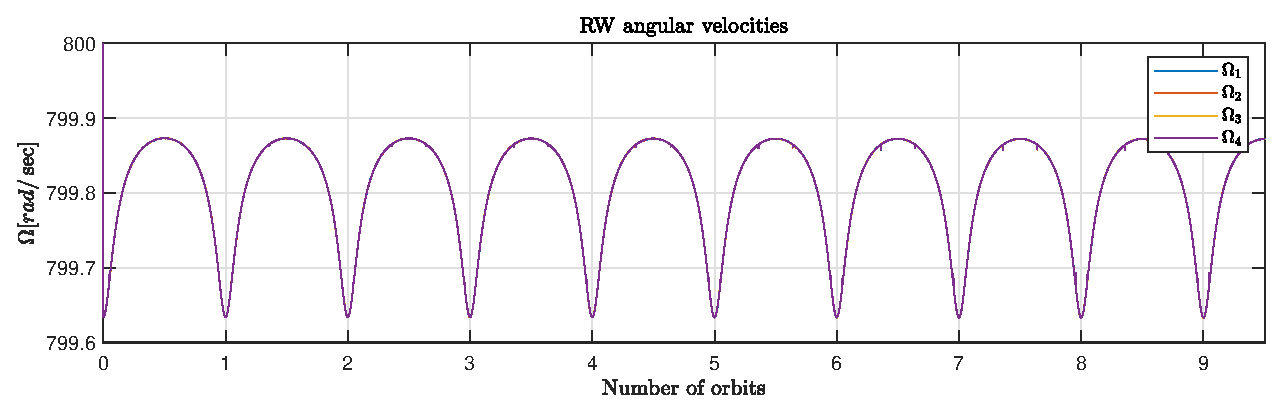
\includegraphics[width=0.9\columnwidth]{figures/plots/VSCMG/vs_ref_mol_Om.eps}
    \caption{RW angular velocity for trajectory tracking maneuver}
    \label{plt:vs_ref_mol_Om}
\end{figure}

From the results, it is clear that VSCMG based ACS are more beneficial than RW based and CMG based ACS. Clear advantages of VSCMG are listed below.

\begin{enumerate}
    \item VSCMG does not poses problem of singularities.
    \item they can produce large torque amplification like CMG,
    \item are able to steer away from singular state by using RWs.
    \item Moreover, Operation is smooth and gimbal rates are within permissible range and no impulsive motion or chattering occurs thus does not poses threat to mechanical integrity of system.
\end{enumerate}

Verified dynamics of VSCMG is further implemented in to standalone environment in C++ with Runge–Kutta ODE solver for integration. This environment is used for training Neural Network based steering law through reinforcement learning explained in next Chapter.
%\part{Artificial Intelligence}
% Neural Network

\chapter{Neural Network based Learning Agent}
\label{chap:6}
In this chapter Artificial Intelligence based agent particularly Neural Network strategy is proposed to evaluate steering of variable speed control moment gyroscope. Machine learning scheme especially reinforcement learning with combination of supervised learning is followed to train neural network \ From equations of motion and control architecture derived in it is evident that spacecraft attitude dynamics is nonlinear function of its states. Moreover singularity avoidance steering mechanism is complex and computationally expensive. Neural network are capable of approximating nonlinear functions and produce sub-optimal solution which is beneficial to reduce computational loads moreover steering is possible without matrix inversion. To design complete neural network based ACS following sections are discussed to clear some concepts. Starting with a brief introduction about machine learning types, particular interest of this thesis is focused on policy gradient method especially Proximal Policy Optimisation is discussed in detail.

\section{Machine Learning}
Machine learning is sub domain of AI is strategy to solve specific task without explicitly programming details of system. Strategy or plan is learned through available labeled data sets. Basically a black box model is approximated \ by studying large amount of input associated output, exploring unlabeled data or by enumerating inputs and outputs of black box function. Based on strategy machine learning is classified in three major parts and their a
application is shown in figure.
\begin{figure}
    \centering
    \scalebox{.5}{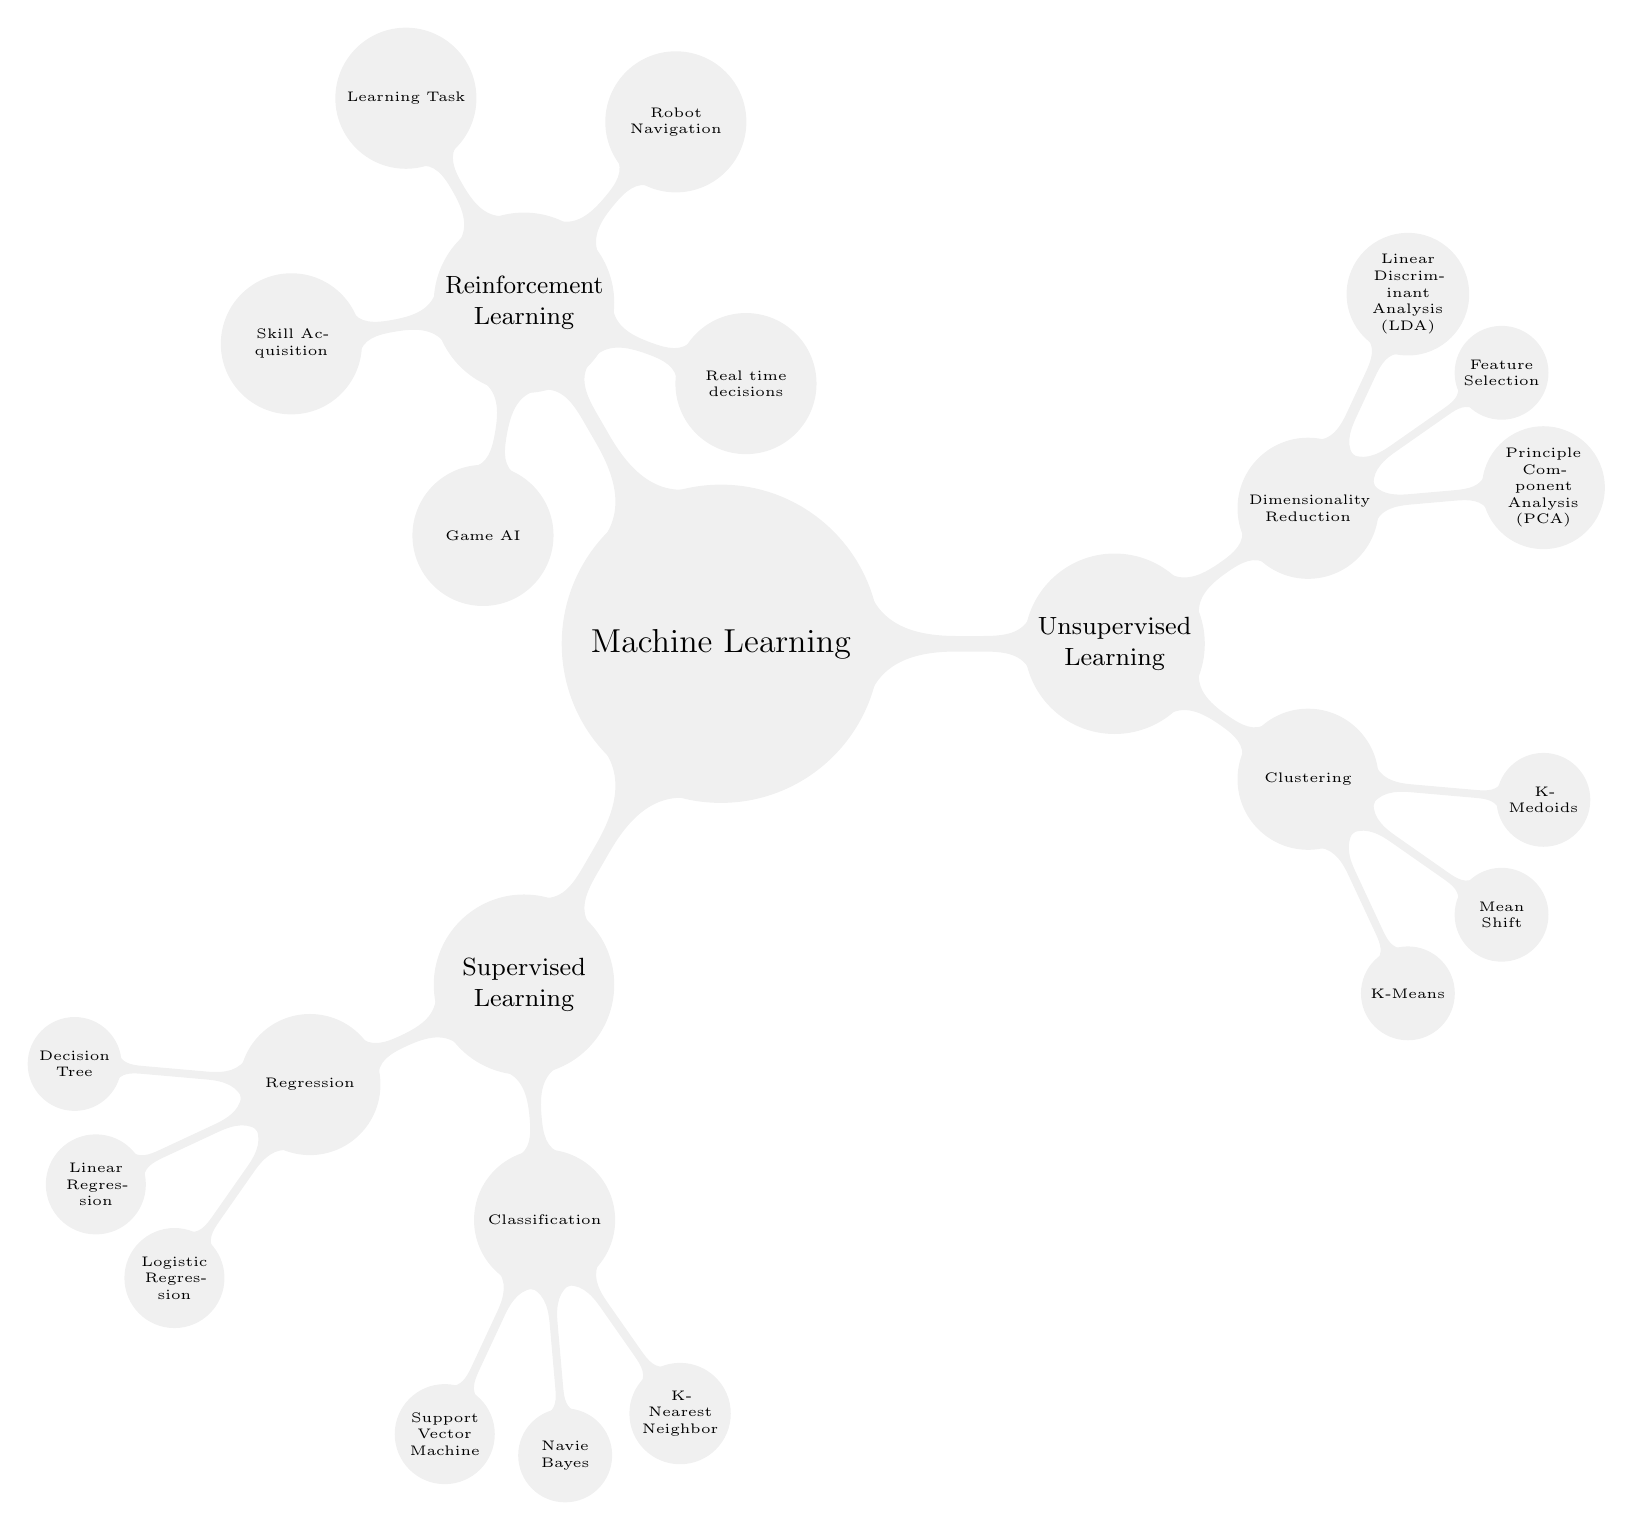
\begin{tikzpicture}[mindmap, grow cyclic, every node/.style=concept, concept color=gray!10, 
	level 1/.append style={font=\small,level distance=5cm,sibling angle=120},
	level 2/.append style={font=\tiny,level distance=3cm,sibling angle=70},
	level 3/.append style={font=\tiny,font=\tiny,level distance=3cm,sibling angle=30},]


\node{Machine Learning}
child { node {Supervised Learning}
    child { node {Regression}
        child { node {Decision Tree}}
        child { node {Linear Regression}}
        child { node {Logistic Regression}} }
    child { node {Classification}
        child { node {Support Vector Machine}}
        child { node {Navie Bayes}}
        child { node {K-Nearest Neighbor}} }
    }
child { node {Unsupervised Learning}
    child { node {Clustering}
        child { node {K-Means}}
        child { node {Mean Shift}}
        child { node {K-Medoids}} }
    child { node {Dimensionality Reduction}
        child { node {Principle Component Analysis (PCA)}}
        child { node {Feature Selection}}
        child { node {Linear Discriminant Analysis (LDA)}} }
    }
child { node {Reinforcement Learning}
        child { node {Real time decisions}}
        child { node {Robot Navigation}}
        child { node {Learning Task}}
        child { node {Skill Acquisition}}
        child { node {Game AI}}
    };

\end{tikzpicture}}
    \caption{Machine Learning Classifications}
    \label{fig:ML_Mindmap}
\end{figure}
\subsection{Supervised Learning}
In this strategy labeled output for particular inputs are known and agent learns relation from input and output mostly used in predictive analysis. Explicitly defined labels are needed hence the name. Model predicts output based on current input and later compare it with labeled output. Two types of supervised learning are classification with categorical output and reparation with numerical output such as fitting a curve. In this thesis supervised learning is used to partially learn strategy from data set produced using steering law discussed in previous chapter in order to reduce training time.

\subsection{Unsupervised Learning}
Machine learns by exploring large chunk of unlabeled data set. Clustering and dimensionality reduction are two sub-classes of unsupervised learning. In this case information is retrieved from data set with keeping simpler and spars representation than original data, can be used to discover pasterns in given data-set. In pattern recognition similar data samples are clustered together.

\newacronym{mdp}{MDP}{Markov Decision Processes}
\subsection{Reinforcement Learning}
Reinforcement learning is a close loop problem where agent takes action, each action is associated with reward or penalty, and based on outcome agent tries to maximize reward or minimize the penalty by exploring in to environment or exploiting past experiences through trial and error along with received feedback. \autoref{fig:ai_agent_env_mdp} shows architecture of agent-environment interaction in \acrlong{mdp}.\cite{russell2010artificial}

\begin{figure}[H]
    \centering

\tikzset{
  frame/.style={
    rectangle, draw,
    text width=6em, text centered,
    minimum height=4em,drop shadow,fill=white,
    rounded corners,
  },
  line/.style={
    draw, -{Latex},rounded corners=0.5mm,
  }
}
\begin{tikzpicture}[font=\small\sffamily\bfseries,very thick,node distance = 4cm]
\node [frame] (agent) {Agent};
\node [frame, below=1.2cm of agent] (environment) {Environment};
\draw[line] (agent) -- ++ (3.5,0) |- (environment)
node[right,pos=0.25,align=left] {action\\ $a_t$};
\coordinate[left=8mm of environment] (P);
\coordinate[above=3mm of environment.west] (ENW);
\coordinate[below=3mm of environment.west] (ESW);
\coordinate[above=3mm of agent.west] (ANW);
\coordinate[below=3mm of agent.west] (ASW);
\draw[thin,dashed] (P|-environment.north) -- (P|-environment.south);
\draw[line] (ESW) -- (P |- ESW)
node[midway,above]{$s_{i+1}$};
\draw[line,thick] (ENW) -- (P |- ENW)
node[midway,above]{$a_{i+1}$};
\draw[line] (P |- ESW) -- ++ (-1.4,0) |- (ANW)
node[left, pos=0.25, align=right] {state\\ $s_t$};
\draw[line,thick] (P |- ENW) -- ++ (-0.8,0) |- (ASW)
node[right,pos=0.25,align=left] {reward\\ $r_t$};
\end{tikzpicture}

    \caption{The agent-environment interaction in  interaction in a Markov Decision Process. \cite{sutton2018reinforcement}}
    \label{fig:ai_agent_env_mdp}
\end{figure}

\noindent\textbf{Agent} is any entity that perceives environment using sensors and acts on it using actuators. A rational agent should take appropriate actions based on strategy to reach goal. Success of agent is determined by performance measure.
Agent function that maps precept history to action is given as:
\begin{equation}
    f: \mathcal{P}^*\longrightarrow \mathcal{A}
\end{equation}
\textbf{Environment} is a real situation or simulated plant dynamics and may have properties such fully or partially observable, deterministic or stochastic, discrete or continuous.
\textbf{Perceptions} are observed states $s\in \mathcal{S}$ in the environment through sensors whereas \textbf{actions} $a\in \mathcal{A}$ are performed by agent through actuators
Agent at state $s$ inside environment, chooses one action $a$ among many choices in order to evolve its state and evolution is determined by state transition probability. For each action, environment provides reward $r \in \mathcal{R}$ as feedback. The \acrfull{mdp} consists of set of states $\mathcal{S}$, set of actions $\mathcal{A}$, transition probability function $P$ reward function $R$, discounting factor for future rewards $\gamma$
\begin{equation*}
    \mathcal{M} = \langle \mathcal{S}, \mathcal{A}, P, R, \gamma \rangle
\end{equation*}
\noindent A \textbf{Policy} $\pi(s)$  is, therefore, a strategy that an agent uses in pursuit of goals.\cite{russell2010artificial} Policy determines actions that has to be taken by agent at state $s$. Policy can be deterministic: $\pi(s)=a$ or stochastic:$\pi(a \vert s) = \mathbb{P}_\pi [A=a \vert S=s]$

Each state is associated with a \textbf{Value} $V(s)$ function which is probability of future rewards than can be received by acting on policy at given state. With future reward as total some of rewards going forward from time t noted as $G_t$
\begin{equation}
    G_t = R_{t+1} + \gamma R_{t+2} + \dots = \sum_{k=0}^{\infty} \gamma^k R_{t+k+1}
\end{equation}
Here discount factor $\gamma \in [0,1]$ is introduced to  penalize the future rewards since propagation of uncertainty becomes larger for long time. The state value is expected return at given state:
\begin{equation}
    V_{\pi}(s) = \mathbb{E}_{\pi}[G_t \vert S_t = s] = \sum_{a \in \mathcal{A}} Q_{\pi}(s, a) \pi(a \vert s)
\end{equation}
Where, action-value of state action pair
\begin{equation}
Q_{\pi}(s, a) = \mathbb{E}_{\pi}[G_t \vert S_t = s, A_t = a]    
\end{equation}
\textbf{Advantage function} $A(s,a)$ is difference between state-value and action value, it asses quality of selected action with respect to certain state.  
\begin{equation}
    A_{\pi}(s, a) = Q_{\pi}(s, a) - V_{\pi}(s)
\end{equation}
An optimum value function that produces maximum returns is
\begin{equation}
    V_{*}(s) = \max_{\pi} V_{\pi}(s),
Q_{*}(s, a) = \max_{\pi} Q_{\pi}(s, a)
\end{equation}
and the policy that achieves optimum value function is optimal policy given as
\begin{equation}
    \pi_{*} = \arg\max_{\pi} V_{\pi}(s),
\pi_{*} = \arg\max_{\pi} Q_{\pi}(s, a)
\end{equation}
The agent-environment interaction is produces series of state, action and reward each time step evolved from $t=0,1,2,\dots,T$. Hence, evolution is sequence state $S_t \in \mathcal{S}$, action $A_t \in \mathcal{A}(s)$ and rewards $R_{t+1} \in \mathcal{R}$ taken at each time $t$ to end of an episode at terminal time $T$.
\acrlong{mdp} shown in \autoref{fig:ai_agent_env_mdp} gives rise to sequence:
\begin{equation*}
    S_0, A_0, R_1,S_1, A_1, R_2, \dots S_{T}, A_{T}, R_{T+1},
\end{equation*}
The model is function that describes environment with associated transition probability $P$ and reward function $R$. Evaluation from state $s$ to next state $s'$ fro action $a$ and associated reward $r$ is transition step and represented as tuple $(s,a,s',r)$. The probability of transition ${\displaystyle s\xrightarrow[a]{} s'}$ is given as
\begin{equation}
P(s',r|s,a)=\mathbb{P} [S_{t+1} =s',R_{t+1} =r|S_{t} =s,A_{t} =a]
\end{equation}
state transition matrix as function of $\displaystyle P(s',r|s,a)$:
\begin{equation}
P^{a}_{ss'} =P(s'|s,a)=\mathbb{P} [S_{t+1} =s'|S_{t} =s,A_{t} =a]=\sum _{r\in \mathcal{R}} P(s',r|s,a)
\end{equation}
and reward function that predicts next reward upon action is
\begin{equation*}
R(s,a)=\mathbb{E} [R_{t+1} |S_{t} =s,A_{t} =a]=\sum _{r\in \mathcal{R}} r\sum _{s'\in \mathcal{S}} P(s',r|s,a)
\end{equation*}


In MDP future only depends on current state and does not have effects of history.
\begin{equation}
\mathbb{P} [S_{t+1} |S_{t} ]=\mathbb{P} [S_{t+1} |S_{1} ,\dotsc ,S_{t} ]
\end{equation}

Decomposition of value function in to immediate reward and the discounted future values using Bellman Equations as
\begin{equation}
\begin{aligned}
V(s) & =\mathbb{E} [G_{t} |S_{t} =s]\\
 & =\mathbb{E} [R_{t+1} +\gamma R_{t+2} +\gamma ^{2} R_{t+3} +\dotsc |S_{t} =s]\\
 & =\mathbb{E} [R_{t+1} +\gamma (R_{t+2} +\gamma R_{t+3} +\dotsc )|S_{t} =s]\\
 & =\mathbb{E} [R_{t+1} +\gamma G_{t+1} |S_{t} =s]\\
 & =\mathbb{E} [R_{t+1} +\gamma V(S_{t+1} )|S_{t} =s]
\end{aligned}
\end{equation}
and action value also referred as Q value is 
\begin{equation}
\begin{aligned}
Q(s,a) & =\mathbb{E} [R_{t+1} +\gamma V(S_{t+1} )\mid S_{t} =s,A_{t} =a]\\
 & =\mathbb{E} [R_{t+1} +\gamma \mathbb{E}_{a\sim \pi } Q(S_{t+1} ,a)\mid S_{t} =s,A_{t} =a]
\end{aligned}
\end{equation}


\section{Policy Gradient Methods}
In order to solve RL problem that is to find optimal strategy with which agent achieves optimal rewards. Policy Gradient Method \cite{Grondman2012} learns with parametrized function of $\displaystyle \theta ,\pi _{\theta } (a|s)$. The reward value depends on the policy and learning is done through optimizing $\displaystyle \theta $ for best rewards. The reward function is defined as:
\begin{equation}
J(\theta )=\sum _{s\in \mathcal{S}} d^{\pi } (s)V^{\pi } (s)=\sum _{s\in \mathcal{S}} d^{\pi } (s)\sum _{a\in \mathcal{A}} \pi _{\theta } (a|s)Q^{\pi } (s,a)
\end{equation}
here \ $\displaystyle d^{\pi }$ is the stationary distribution of Markov chain for $\displaystyle \pi _{\theta }$. The idea is for by exploring states of

Markov chain for long period of time, probability of conversing to one state becomes constant and known as stationary probability for $\displaystyle \pi _{\theta }$. Starting from initial state $\displaystyle s_{0}$ up to state $\displaystyle s_{t}$ with using policy $\displaystyle \pi _{\theta }$ the stationary distribution \ $\displaystyle d^{\pi }$ is given as:
\begin{equation}
d^{\pi } (s)=\lim _{t\rightarrow \infty } P(s_{t} =s|s_{0} ,\pi _{\theta } )
\end{equation}


Now with using gradient ascent search for best $\displaystyle \theta $ that gives maximum rewards.

\subsection{Policy Gradient Theorem}
Consider the $\displaystyle \theta $ with $\displaystyle k$ dimensions is to be optimized, numerical gradient of $\displaystyle \theta $ can be found with \ introducing small perturbation $\displaystyle \epsilon $ 
\begin{equation}
\frac{\partial J(\theta )}{\partial \theta _{k}} \approx \frac{J(\theta +\epsilon u_{k} )-J(\theta )}{\epsilon }
\end{equation}
 and for analytical gradient of \ $\displaystyle J(\theta )$
\begin{equation}
\begin{aligned}
J(\theta ) & =\sum _{s\in \mathcal{S}} d(s)\sum _{a\in \mathcal{A}} \pi (a|s,\theta )Q_{\pi } (s,a)\\
\nabla J(\theta ) & =\sum _{s\in \mathcal{S}} d(s)\sum _{a\in \mathcal{A}} \nabla \pi (a|s,\theta )Q_{\pi } (s,a)\\
 & =\sum _{s\in \mathcal{S}} d(s)\sum _{a\in \mathcal{A}} \pi (a|s,\theta )\frac{\nabla \pi (a|s,\theta )}{\pi (a|s,\theta )} Q_{\pi } (s,a)\\
 & =\sum _{s\in \mathcal{S}} d(s)\sum _{a\in \mathcal{A}} \pi (a|s,\theta )\nabla \ln \pi (a|s,\theta )Q_{\pi } (s,a)\\
 & =\mathbb{E}_{\pi _{\theta }} [\nabla \ln \pi (a|s,\theta )Q_{\pi } (s,a)]
\end{aligned}
\end{equation}
and finally, we get policy gradient theorem as
\begin{equation}
\nabla J(\theta )=\mathbb{E}_{\pi _{\theta }} [\nabla \ln \pi (a|s,\theta )Q_{\pi } (s,a)]
\end{equation}
Since probabilities of each actions are not computed,policy gradient methods are suitable for continuous action space.

\subsection{Proximal Policy Optimization (PPO)}
Proposed by John et. al. PPO\cite{schulman2017proximal} which optimizes a clipped/surrogate objective function using stochastic gradient ascent. In this method multiple epochs of mini batch updates are used instead of one update per batch. Let consider probability ratio of old and new policies as:
\begin{equation}
r(\theta )=\frac{\pi _{\theta } (a|s)}{\pi _{\theta _{\text{old}}} (a|s)}
\end{equation}

\noindent then objective function of TRPO\footnote{Trust Region Policy Optimization\cite{schulman2015trust} avoids parameter updates that change the policy rapidly} is reduced to
\begin{equation}
J^{TRPO} (\theta )=\mathbb{E}[ r(\theta )\hat{A}_{\theta _{old}} (s,a)]
\end{equation}
if distance between $\displaystyle \theta _{old}$ and $\displaystyle \theta $ is not limited, extremely large parameter updates will be made to optimize $\displaystyle J^{TRPO}( \theta )$, leading to instability. In PPO $\displaystyle r( \theta )$ is bounded close to $\displaystyle 1\pm \epsilon $, here $\displaystyle \epsilon $ is hyperparameter and minimum of either same objective or clipped objective is selected.
\begin{equation}
J^{CLIP} (\theta )=\mathbb{E} [\min (r(\theta )\hat{A}_{\theta _{old}} (s,a),clip(r(\theta ),1-\epsilon ,1+\epsilon )\hat{A}_{\theta _{old}} (s,a))]
\end{equation}
ratio $\displaystyle r( \theta )$ is clipped between $\displaystyle 1-\epsilon $ and $\displaystyle 1+\epsilon $ as shown in \autoref{fig:ppo_cliped} surrogate $J^{CLIP}(\theta)$ as function of probability ratio $r$ for one step starting from $r=1$. since ratio is clipped and does not vary rapidly large policy updates are skipped hence increasing stability. \autoref{algo_PPO_AC} is actor critic style parallel implementation of PPO.

\begin{figure}[H]
    \centering
    

\tikzset{every picture/.style={line width=0.75pt}} %set default line width to 0.75pt        

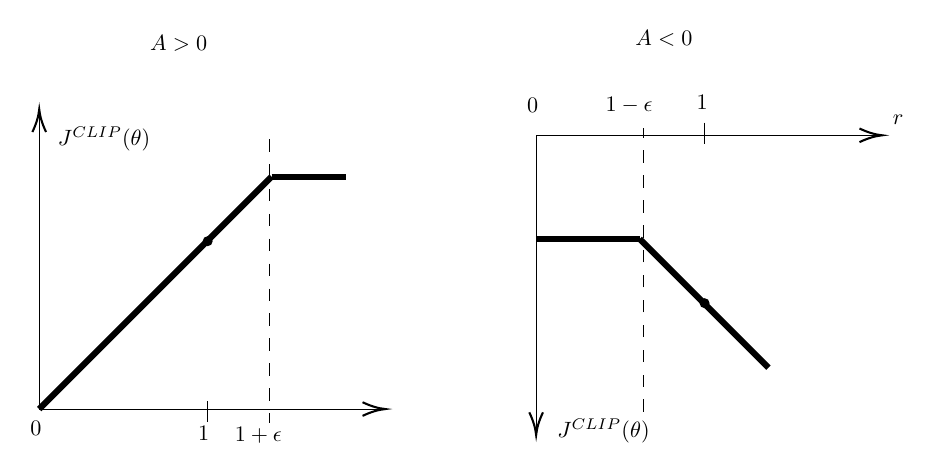
\begin{tikzpicture}[x=0.75pt,y=0.75pt,yscale=-1,xscale=1]
%uncomment if require: \path (0,283); %set diagram left start at 0, and has height of 283

%Straight Lines [id:da07428987415964317] 
\draw    (60.04,246.51) -- (60.04,104.1) ;
\draw [shift={(60.04,102.1)}, rotate = 450] [color={rgb, 255:red, 0; green, 0; blue, 0 }  ][line width=0.75]    (10.93,-3.29) .. controls (6.95,-1.4) and (3.31,-0.3) .. (0,0) .. controls (3.31,0.3) and (6.95,1.4) .. (10.93,3.29)   ;
%Straight Lines [id:da42162293191171707] 
\draw    (60.04,246.51) -- (224.76,246.51) ;
\draw [shift={(226.76,246.51)}, rotate = 180] [color={rgb, 255:red, 0; green, 0; blue, 0 }  ][line width=0.75]    (10.93,-3.29) .. controls (6.95,-1.4) and (3.31,-0.3) .. (0,0) .. controls (3.31,0.3) and (6.95,1.4) .. (10.93,3.29)   ;
%Straight Lines [id:da46857481861880057] 
\draw  [dash pattern={on 4.5pt off 4.5pt}]  (170.93,116.45) -- (170.93,253.43) ;
%Straight Lines [id:da5916594745882346] 
\draw [line width=2.25]    (60.04,246.51) -- (171.98,134.58) ;
%Straight Lines [id:da20769803027157696] 
\draw [line width=2.25]    (171.98,134.58) -- (208.01,134.58) ;
%Shape: Ellipse [id:dp9944817970164661] 
\draw  [fill={rgb, 255:red, 0; green, 0; blue, 0 }  ,fill opacity=1 ] (139.07,165.63) .. controls (139.07,164.46) and (140.02,163.51) .. (141.19,163.51) .. controls (142.36,163.51) and (143.31,164.46) .. (143.31,165.63) .. controls (143.31,166.8) and (142.36,167.75) .. (141.19,167.75) .. controls (140.02,167.75) and (139.07,166.8) .. (139.07,165.63) -- cycle ;
%Straight Lines [id:da631388526485618] 
\draw    (141.19,252.63) -- (141.19,242.51) ;
%Straight Lines [id:da5700736740675836] 
\draw    (299.45,114.62) -- (299.45,257.03) ;
\draw [shift={(299.45,259.03)}, rotate = 270] [color={rgb, 255:red, 0; green, 0; blue, 0 }  ][line width=0.75]    (10.93,-3.29) .. controls (6.95,-1.4) and (3.31,-0.3) .. (0,0) .. controls (3.31,0.3) and (6.95,1.4) .. (10.93,3.29)   ;
%Straight Lines [id:da4383859714024194] 
\draw    (299.45,114.62) -- (464.17,114.62) ;
\draw [shift={(466.17,114.62)}, rotate = 540] [color={rgb, 255:red, 0; green, 0; blue, 0 }  ][line width=0.75]    (10.93,-3.29) .. controls (6.95,-1.4) and (3.31,-0.3) .. (0,0) .. controls (3.31,0.3) and (6.95,1.4) .. (10.93,3.29)   ;
%Straight Lines [id:da15252831399229727] 
\draw [line width=2.25]    (349.38,164.55) -- (411.38,226.55) ;
%Straight Lines [id:da20676916509391385] 
\draw [line width=2.25]    (299.29,164.55) -- (349.38,164.55) ;
%Shape: Ellipse [id:dp5844715267834208] 
\draw  [fill={rgb, 255:red, 0; green, 0; blue, 0 }  ,fill opacity=1 ] (378.47,195.5) .. controls (378.47,196.67) and (379.42,197.62) .. (380.59,197.62) .. controls (381.77,197.62) and (382.72,196.67) .. (382.72,195.5) .. controls (382.72,194.33) and (381.77,193.38) .. (380.59,193.38) .. controls (379.42,193.38) and (378.47,194.33) .. (378.47,195.5) -- cycle ;
%Straight Lines [id:da16120535517562784] 
\draw    (380.59,108.5) -- (380.59,118.62) ;
%Straight Lines [id:da12247292832159551] 
\draw  [dash pattern={on 4.5pt off 4.5pt}]  (350.97,247.88) -- (350.97,110.91) ;

% Text Node
\draw (470.29,103.87) node [anchor=north west][inner sep=0.75pt]  [xscale=0.8,yscale=0.8]  {$r$};
% Text Node
\draw (68.02,109.38) node [anchor=north west][inner sep=0.75pt]  [xscale=0.8,yscale=0.8]  {$J^{CLIP}( \theta )$};
% Text Node
\draw (135.61,253.59) node [anchor=north west][inner sep=0.75pt]  [xscale=0.8,yscale=0.8]  {$1$};
% Text Node
\draw (153.24,254.39) node [anchor=north west][inner sep=0.75pt]  [xscale=0.8,yscale=0.8]  {$1+\epsilon $};
% Text Node
\draw (112.41,65.43) node [anchor=north west][inner sep=0.75pt]  [xscale=0.8,yscale=0.8]  {$A >0$};
% Text Node
\draw (308.62,250.38) node [anchor=north west][inner sep=0.75pt]  [xscale=0.8,yscale=0.8]  {$J^{CLIP}( \theta )$};
% Text Node
\draw (375.82,94.26) node [anchor=north west][inner sep=0.75pt]  [xscale=0.8,yscale=0.8]  {$1$};
% Text Node
\draw (331.89,95.06) node [anchor=north west][inner sep=0.75pt]  [xscale=0.8,yscale=0.8]  {$1-\epsilon $};
% Text Node
\draw (294.15,95.86) node [anchor=north west][inner sep=0.75pt]  [xscale=0.8,yscale=0.8]  {$0$};
% Text Node
\draw (54.74,251.19) node [anchor=north west][inner sep=0.75pt]  [xscale=0.8,yscale=0.8]  {$0$};
% Text Node
\draw (346.2,63.03) node [anchor=north west][inner sep=0.75pt]  [xscale=0.8,yscale=0.8]  {$A< 0$};


\end{tikzpicture}    \caption{Surrogate $J^{CLIP}(\theta)$as function of probability ratio for positive (left) and negative (right) advantage, figure reconstructed from original paper. \cite{schulman2017proximal}}
    \label{fig:ppo_cliped}
\end{figure}


\begin{algorithm}[H]
\SetAlgoLined
\KwResult{Write here the result }
\For{iteration=$1,2,\dots$} {
\For{actor=$1,2,\dots,N$} {
Run policy $\displaystyle \pi_{\theta_{old}}$ in environment for $T$ time steps.\\
Compute advantage estimates $\hat{A}_1,\dots,\hat{A}_T$
}
Optimize surrogate $L$ wrt $\theta$, with $K$ epochs and minibatch size $M \leq NT$ \\
$\theta_{old} \xleftarrow[]{} \theta$
}
 \caption{PPO,Actor-Critic Style}
    \label{algo_PPO_AC}
\end{algorithm}
\section{Neural Network}
Neural networks were first introduced  in 1944 by Warren McCullough and Walter Pitts. Inspired by human brain neural networks are large graphs made up of densely connected processing nodes. Theses processing nodes are referred as neurons, It may take multiple inputs and produce one output. Each input $x_i$ is associated with some weight $w_i$, neuron produces weighted some of inputs adds bias to it and squeezes the results with pre-selected activation function. As shown in \autoref{fig:neuron} neuron functions as
\begin{equation}
    y_{out} = f(b+\sum ^{n}_{i=1} x_i,w_i)
\end{equation}
\begin{figure}[H]
    \centering
    
    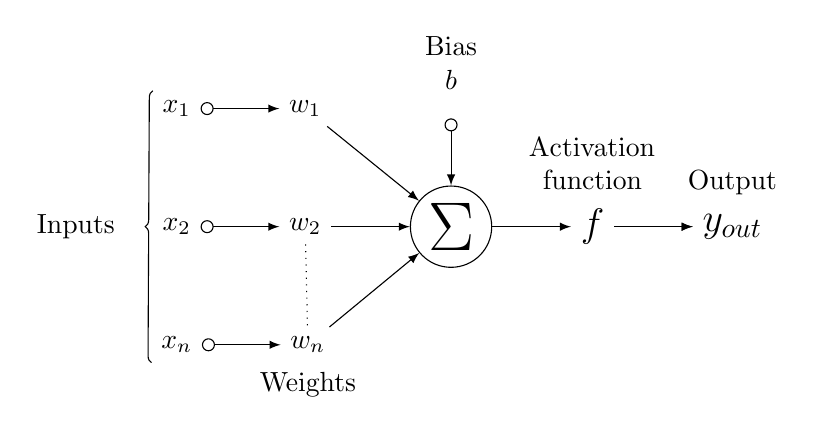
\begin{tikzpicture}[
    % define styles    
    init/.style={ 
         draw, 
         circle, 
         inner sep=2pt,
         font=\Huge,
         join = by -latex
    },
    squa/.style={ 
        font=\Large,
        join = by -latex
    }
]
% Top chain x1 to w1
\begin{scope}[start chain=1]
    \node[on chain=1] at (0,1.5cm)  (x1) {$x_1$};
    \node[on chain=1,join=by o-latex] (w1) {$w_1$};
\end{scope}
% Middle chain x2 to output
\begin{scope}[start chain=2]
    \node[on chain=2] (x2) {$x_2$};
    \node[on chain=2,join=by o-latex](w2) {$w_2$};
    \node[on chain=2,init] (sigma) {$\displaystyle\Sigma$};
    \node[on chain=2,squa,label=above:{\parbox{2cm}{\centering Activation\\ function}}]   {$f$};
    \node[on chain=2,squa,label=above:Output,join=by -latex] {$y_{out}$};
\end{scope}
% Bottom chain x3 to w3
\begin{scope}[start chain=3]
    \node[on chain=3] at (0,-1.5cm) 
    (x3) {$x_n$};
    \node[on chain=3,label=below:Weights,join=by o-latex]
    (w3) {$w_n$};
\end{scope}
% Bias
\node[label=above:\parbox{2cm}{\centering Bias \\ $b$}] at (sigma|-w1) (b) {};
% Arrows joining w1, w3 and b to sigma
\draw[-latex] (w1) -- (sigma);
\draw[-latex] (w3) -- (sigma);
\draw[o-latex] (b) -- (sigma);

\draw[dotted](w2) -- (w3);

% left hand side brace
\draw[decorate,decoration={brace,mirror}] (x1.north west) -- node[left=10pt] {Inputs} (x3.south west);

\end{tikzpicture}
    \caption{Components of individual Neuron.The activation function is denoted by $f$ and applied on the weighted sum of inputs with added bias}
    \label{fig:neuron}
\end{figure}
\noindent Activation function is basically squeezing of weighted sum in to some allowable values, sometimes activation can be just an trigger which occurs after reaching decided threshold. Shapes of commonly used activation functions are shown in \autoref{fig:act_func}. Apart from its shape most important property of activation function is its derivative which has crucial role for training a neural network. Few commonly used activation functions are mentioned in \autoref{tbl_act_func}

\begin{figure}[H]
\centering
 \begin{subfigure}[t]{0.45\columnwidth}
 \centering
         
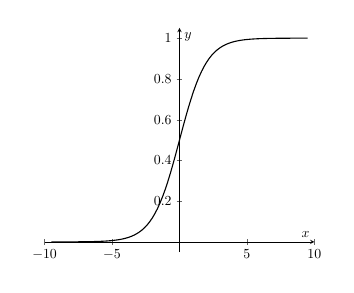
\begin{tikzpicture}[scale = 0.5]
\begin{axis}[
    axis lines=middle,
    xmax=10,
    xmin=-10,
    ymin=-0.05,
    ymax=1.05,
    xlabel={$x$},
    ylabel={$y$}
]
\addplot [domain=-9.5:9.5, samples=100,
          thick, black] {1/(1+exp(-x)};
\end{axis}
\end{tikzpicture}

 \caption{Sigmoid}
 \label{fig:act_sigmoid}
 \end{subfigure}
~ 
 \begin{subfigure}[t]{0.45\columnwidth}
 \centering

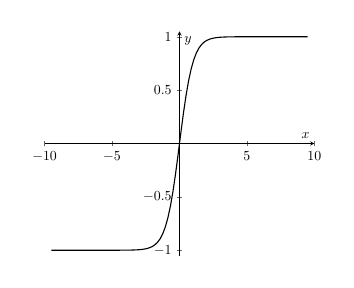
\begin{tikzpicture}[scale = 0.5]
\begin{axis}[
    axis lines=middle,
    xmax=10,
    xmin=-10,
    ymin=-1.05,
    ymax=1.05,
    xlabel={$x$},
    ylabel={$y$}]
\addplot [domain=-9.5:9.5, samples=100,
     thick, black] {(exp(x) - exp(-x))/(exp(x) + exp(-x))};
\end{axis}
\end{tikzpicture}

 \caption{tanh}
 \label{fig:act_tanh}
 \end{subfigure}
~ 
 \begin{subfigure}[t]{0.45\columnwidth}
 \centering

\begin{tikzpicture}[scale = 0.5]
\begin{axis}[
    axis lines=middle,
    xmax=6,
    xmin=-6,
    ymin=-0.05,
    ymax=5.05,
    xlabel={$x$},
    ylabel={$y$}]
\addplot [domain=-5.5:5.5, samples=100, thick, black] {max(0, x)};
\end{axis}
\end{tikzpicture}

 \caption{ReLu}
 \label{fig:act_relu}
 \end{subfigure}
~ 
 \begin{subfigure}[t]{0.45\columnwidth}
 \centering
\begin{tikzpicture}[scale = 0.5]
\begin{axis}[
    axis lines=middle,
    xmax=6,
    xmin=-6,
    ymin=-1.05,
    ymax=5.05,
    xlabel={$x$},
    ylabel={$y$}]
\addplot [domain=-5.5:5.5, samples=100,
          thick, black] {max(0.1 * x, x)};
\end{axis}
\end{tikzpicture}
\caption{Leaky ReLu}
\label{fig:act_leackrelu}
     \end{subfigure}
     
\caption{Commonly used activation functions}
\label{fig:act_func}
\end{figure}


\begin{table}[H]
        \centering
\begin{tabular}{p{0.3\textwidth}|p{0.3\textwidth}|p{0.3\textwidth}}
\toprule
 Activation Function & Function $\displaystyle f(z)$ & Derivative $\displaystyle f'(z)$ \\
\midrule
 Sigmoid & {\small $\displaystyle f(z)=\frac{1}{1+e^{-z}}$} & {\small $\displaystyle f'( z) \ =\ f( z) \ \cdotp ( 1\ -\ f( z))$} \\
\hline 
 Tanh & {\small $\displaystyle f(z)=\frac{e^{z} -e^{-z}}{e^{z} +e^{-z}}$} & {\small $\displaystyle f'(z)=1-\tanh (z)^{2}$} \\
\hline 
 Linear & {\small $\displaystyle f( z) =z\alpha $} & {\small $\displaystyle f'( z) =\alpha $} \\
\hline 
 Exponential Linear Unit (ELU) & {\small $\displaystyle f( z) =\begin{cases}
z & z >0\\
\alpha \left( e^{z} -1\right) & z\leq 0
\end{cases}$} & {\small $\displaystyle f'( z) =\begin{cases}
1 & z >0\\
\alpha e^{z} & z\leq 0
\end{cases}$} \\
\hline 
 Rectified Linear Units (ReLU) & {\small $\displaystyle f( z) =\begin{cases}
z & z >0\\
0 & ,z\leq 0
\end{cases}$} & {\small $\displaystyle f'( z) =\begin{cases}
z & z >0\\
0 & z\leq 0
\end{cases}$} \\
\hline 
 LeakyRelu & {\small $\displaystyle f( z) =\begin{cases}
z & z >0\\
\alpha z & z\leq 0
\end{cases}$} & {\small $\displaystyle f'( z) =\begin{cases}
z & z >0\\
\alpha  & z\leq 0
\end{cases}$} \\
\hline 
 Arctan & {\small $\displaystyle f( z) =\tan^{-1}( z)$} & {\small $\displaystyle f'( z) =\frac{1}{1+z^{2}}$} \\
\hline 
 Swish & {\small $\displaystyle f(z)=\frac{z}{1+e^{-z}}$} & {\small $\displaystyle f'(z)=\frac{f( z)( 1-f( z))}{1+e^{-z}}$} \\
\hline 
 Soft Plus & {\small $\displaystyle f(z)=\ln\left( 1+e^{z}\right)$} & {\small $\displaystyle f'(z)=\frac{1}{1+e^{-z}}$} \\

\bottomrule
\end{tabular}
\caption{Commonly used activation functions and their derivative}
\label{tbl_act_func}
\end{table}

\newacronym{mlp}{MLP}{Multi Layer Perceptron}
\subsection{Multi Layer Perceptron policy}
\acrlong{mlp} is a complex network of perceptrons connected based on various architectures. Most common method is feed forward neural network. Neurons are grouped in a single stage called a layers. Every unit in a layer is connected to all units of previous layers. Three distinct layers are Input, Hidden and Output. Data enters from input and passes thorough hidden layers finally emitted from output layer. Hidden layers are not accessible to external world hence the name. Shallow neural network has one hidden layer as opposed to Deep neural networks, which may have multiple hidden layers, an example shown in \autoref{fig:mlp}. With properly chosen weights, Neural network can approximate any nonlinear function. Process of finding weights is called training an iterative process where data is passed from input layer and based on error between evaluated and expected output weights are updated in backward direction layer by layer, process referred as propagation.
\begin{figure}
    \centering
    \scalebox{0.65}{

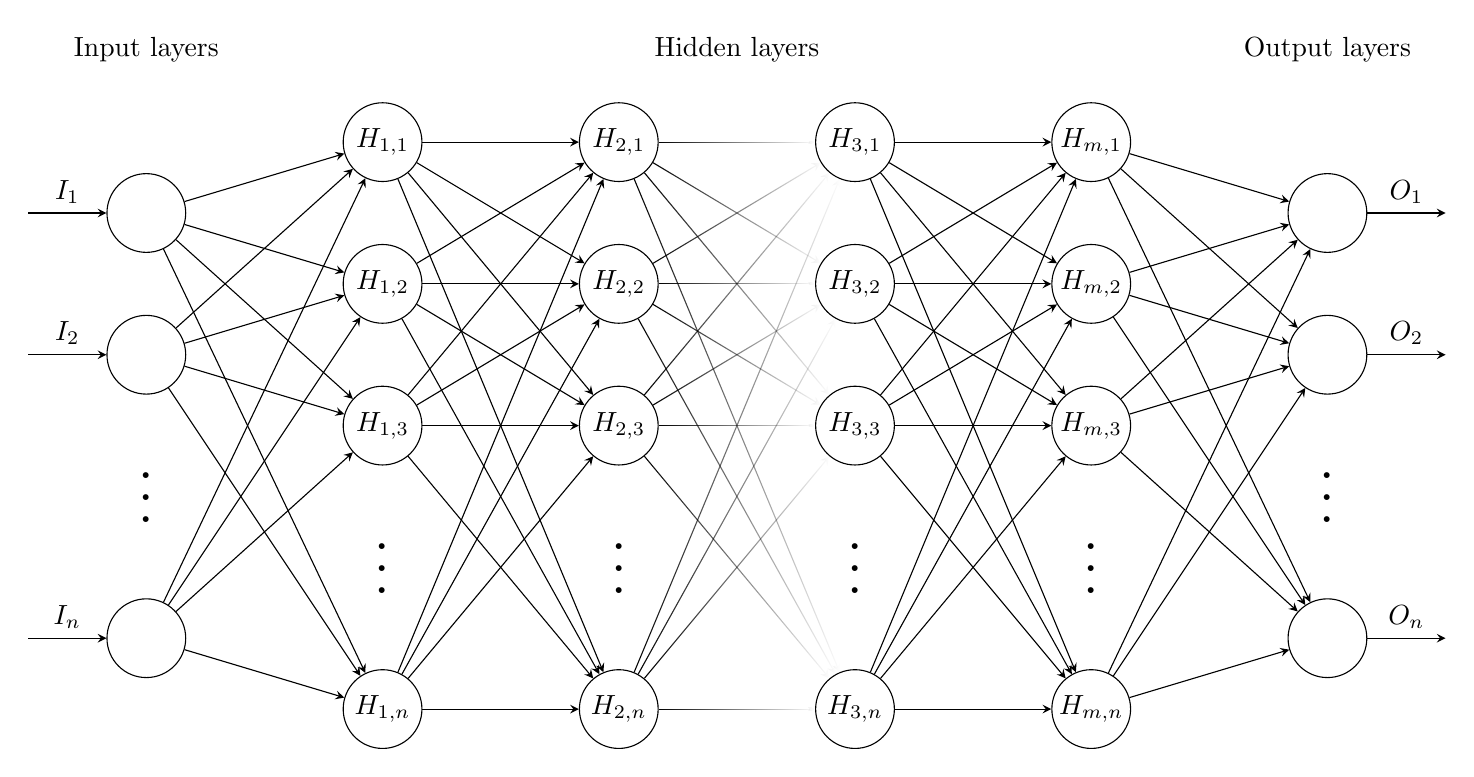
\begin{tikzpicture}[x=1.5cm, y=1.5cm, >=stealth]
\tikzset{%
  every neuron/.style={
    circle,
    draw,
    minimum size=1cm
  },
  neuron missing/.style={
    draw=none, 
    scale=2,
    text height=0.333cm,
    execute at begin node=\color{black}$\vdots$
  },
}
% Input
\foreach \m/\l [count=\y] in {1,2,missing,3}
  \node [every neuron/.try, neuron \m/.try] (input-\m) at (0, 3-\y*1.2) {};
% h1 1
\foreach \m [count=\y] in {1,2,3,missing,4}
  \node [every neuron/.try, neuron \m/.try ] (h1-\m) at (2, 3.6-\y*1.2) {};
% h1 2
\foreach \m [count=\y] in {1,2,3,missing,4}
  \node [every neuron/.try, neuron \m/.try ] (h2-\m) at (4, 3.6-\y*1.2) {};
% h1 3
\foreach \m [count=\y] in {1,2,3,missing,4}
  \node [every neuron/.try, neuron \m/.try ] (h3-\m) at (6, 3.6-\y*1.2) {};

% h1 4
\foreach \m [count=\y] in {1,2,3,missing,4}
  \node [every neuron/.try, neuron \m/.try ] (h4-\m) at (8, 3.6-\y*1.2) {};

% Output
\foreach \m [count=\y] in {1,2,missing,3}
  \node [every neuron/.try, neuron \m/.try ] (output-\m) at (10,3-\y*1.2) {};

\foreach \l [count=\i] in {1,2,n}
  \draw [<-] (input-\i) -- ++(-1,0)
    node [above, midway] {$I_\l$};

\foreach \l [count=\i] in {1,2,3,n}
  \node [] at (h1-\i) {$H_{1,\l}$};

\foreach \l [count=\i] in {1,2,3,n}
  \node [] at (h2-\i) {$H_{2,\l}$};

\foreach \l [count=\i] in {1,2,3,n}
  \node [] at (h3-\i) {$H_{3,\l}$};

\foreach \l [count=\i] in {1,2,3,n}
  \node [] at (h4-\i) {$H_{m,\l}$};

\foreach \l [count=\i] in {1,2,n}
  \draw [->] (output-\i) -- ++(1,0)
    node [above, midway] {$O_\l$};

\foreach \i in {1,...,3}
  \foreach \j in {1,...,4}
    \draw [->] (input-\i) -- (h1-\j);

\foreach \i in {1,...,4}
  \foreach \j in {1,...,4}
    \draw [->] (h1-\i) -- (h2-\j);

\foreach \i in {1,...,4}
  \foreach \j in {1,...,4}
    \draw [->,path fading=east] (h2-\i) -- (h3-\j);


\foreach \i in {1,...,4}
  \foreach \j in {1,...,4}
    \draw [->] (h3-\i) -- (h4-\j);

\foreach \i in {1,...,4}
  \foreach \j in {1,...,3}
    \draw [->] (h4-\i) -- (output-\j);
%
%\foreach \l [count=\x from 1] in {1, 2, 3, n}
%  \node [align=center, above] at (\x*2,3) {Hidden %\l};

\node [align=center, above] at (0,3) {Input layers};
\node [align=center, above] at (5,3) {Hidden layers};
\node [align=center, above] at (10,3) {Output layers};

\end{tikzpicture}}
    \caption{Multi Layer Perceptron}
    \label{fig:mlp}
\end{figure}
Lets recall operation of each neuron with $n$ inputs. 
\begin{equation}
    \hat{y}=f_{act}(b+W_{n\times1}^TX_{n\times1})
\end{equation}

\begin{equation*}
\hat{y} =f_{act}(\vec{w} \cdotp \vec{x} +b)
\end{equation*}
for input vector $\displaystyle \vec{x}$ error between output $\displaystyle \hat{y}$ and expected output $\displaystyle y$ can be computed using Mean Square Error (MSE) for set of $\displaystyle N$ input output pair $\displaystyle X=\{\vec{x}_{i} ,y_{i}\} ,i\in \{1,N\}$as:

\begin{equation}
E( X) =\frac{1}{2N}\sum ^{N}_{i=1}(\hat{y}_{i} -y_{i})^{2} =\frac{1}{2N}\sum ^{N}_{i=1}( f_{act}(\vec{w} \cdotp \vec{x} +b) -y_{i})^{2}
\end{equation}Objective of training is to minimize the error $\displaystyle E( X)$ which can be done with gradient descent
\begin{equation}
\begin{aligned}
\vec{w}_{i+1} & =\vec{w}_{i} -\alpha \frac{\partial E( X)}{\partial \vec{w}_{i}}\\
b_{i+1} & =b_{i} -\alpha \frac{\partial E( X)}{\partial b_{i}}
\end{aligned}
\end{equation}
Here $\displaystyle \alpha $ is learning rate, typically a small value the weight deviation $\displaystyle \Delta \vec{w} =\vec{w}_{i+1} -\vec{w}_{i}$ bias deviation $\displaystyle \Delta b=b_{i+1} -b_{i}$ for iteration is calculated as:
\begin{equation}
\begin{aligned}
\Delta \vec{w} & =\frac{1}{N}\sum ^{N}_{i=1} \alpha (\vec{y}_{i} -\hat{y}_{i}) f'_{act}(\vec{w} \cdotp \vec{x} +b)\vec{x}_{i}\\
\Delta b & =\frac{1}{N}\sum ^{N}_{i=1} \alpha (\vec{y}_{i} -\hat{y}_{i}) f'_{act}(\vec{w} \cdotp \vec{x} +b)
\end{aligned}
\end{equation}
\section{Neural Network based VSCMG steering Law}
Starting with fundamentals discussed in earlier sections, a neural network is trained to solve problem of VSCMG steering. Idea is, for required torque at particular state of spacecraft, what signals should be given to the gimbal and flywheel motors are evaluated from neural network described in \autoref{fig:nn_control_architecture}. 

\begin{figure}[H]
    \centering
    \tikzstyle{block} = [draw, fill=blue!0, rectangle, 
    minimum height=3em, minimum width=5em,align=center]
\tikzstyle{sum} = [draw, fill=blue!0, circle, node distance=1cm]
\tikzstyle{input} = [coordinate]
\tikzstyle{tmp} = [coordinate]
\tikzstyle{output} = [coordinate]
\tikzstyle{pinstyle} = [pin edge={to-,thin,black}]

\begin{tikzpicture}[auto, node distance=2cm,>=latex']
% Boxing and labelling noise shapers
	\draw [color=black,thick,fill={rgb:black,1;white,30}](6.2,1.2) rectangle (11.2,-0.8);
	\node at (6,1) [below=1mm, right=2mm] {{Spacecraft Bus}};
	
    \node [input, name=input] {};
    \node [sum, right of=input](sum) {};
    \node [block, right of=sum, name=ctrl,node distance=1.5cm]
        {Control \\ Law};
    \node [block, right of=ctrl, name=str,node distance=2.5cm]
        {Steering \\ Law};
    \node [block, right of=str,node distance=2.5cm] (cmg)
        {VSCMG \\ Cluster};
    \node [block, right of=cmg,node distance=2.5cm] (sys)
        {Platform \\ Dynamics};
    \node [output,right of=sys,node distance=2cm] (output){};
    
    
    \draw [draw,->] (input) -- node {$r$} (sum);
    \draw[->](sum)--node {$e$}(ctrl);
    \draw[->](ctrl)--node {$\tau_c$}(str);
    \draw[->](str)--node {}(cmg);
    \draw[->](cmg)--node {$\tau_{a}$}(sys);
    \draw[->](sys)-- node [name=y] {$y$}(output);
    \node[tmp,below of=sys,node distance=1.5cm](fo1){};
    \node[tmp,below of=y,node distance=2.5cm](fo2){};
    \draw[->](y)--(fo2)-|node[pos=0.99] {$-$} 
        node [near start] {Spacecraft State feedback}(sum);
    \draw[->](sys)--(fo1)-|node [near start] {VSCMG State feedback}(str);


\end{tikzpicture}

    %\includegraphics{}
    \caption{Neural Network based VSCMG Spacecraft Steering and Control Architecture}
    \label{fig:nn_control_architecture}
\end{figure}
\subsection{Reinforcement Learning Agent}
As previously reported Reinforcement Learning based strategy has an ``Agent'' learns a policy in this case a \acrshort{mlp} policy by interacting with environment in order to maximize the received reward. The observation space of agent is states that agent can precept and action space is actuators that agent can act on. \acrshort{mlp} policy is designed such a way that input layer is observation space and output layer is action space. In order to train the model a critic network is required, input layer of critic is sum observation space and action space while only one output.
\newacronym{dll}{DLL}{Dynamical Linked Library}
\subsection{Training Procedure}
With regard to \autoref{fig:ppo_flowchart} a custom environment with complete VSCMG dynamical equation of motion stepper compatible with OpenAI Gym \cite{OpenAIGym} is developed in python. This environment evolves predefined time-step at each call, although time-steps considered are order of magnitude of milliseconds environment takes multiple intermediate time-steps based on adaptive  Runge–Kutta Cash–Karp method in order to preserve accuracy of numerical integration. After integrating for one step environment returns observations, action, reward and few status parameters for monitoring learning process. It is realised that python based \newacronym{ode}{ODE}{Ordinary Differential Equation} \acrfull{ode} integrator is slow and knowing the fact that simulation time must be in magnitude of millions of seconds, entire equation of motion is developed in C++ with Boost library \cite{abrahams2003building} for high performance \acrshort{ode} integrator. The developed \acrfull{dll} has exported interface with python consequently increasing performance and speed of simulation. Tensorflow and Open Source machine learning library has been used to train the agent. Along with plots of system states, OpenGL based real time 3D visualization of VSCMG is devolved in order to have better understanding of system dynamics. Some core components of VSCMG Environment are 
\subsection{Observation Space}
Choice of observation can be a vector of states comprising quaternion error, body rate error, RW velocities and gimbals angles. Since outer loop is of control remains same, for steering law observation which is input layer of policy layer is selected as vector comprising demand torque, gimbal angles and RW velocities. This reduced length observation space from $\displaystyle 15$ to 11, keeping information of attitude error and rate error in the form of required torque. Selecting reduced observation space also played important role for redaction in storage requirements. Since for supervised learning, large amount of trajectory with input output pairs need to be stored.
\begin{equation}
s_{11\times 1} =\begin{pmatrix}
\mathbf{\tau }_{c}\\
\mathbf{{\delta }}\\
\mathbf{{\Omega }}
\end{pmatrix}
\end{equation}
\subsection{Action Space}
All Reaction wheel angular accelerations, and gimbal velocities are considered as action space which is output layer of Policy network.

\begin{equation}
a_{8\times 1} =\begin{pmatrix}
\mathbf{\dot{\delta }}\\
\mathbf{\dot{\Omega }}
\end{pmatrix}
\end{equation}


\noindent here gimbal velocity and angular acceleration bounded by actuator limit within $\displaystyle \mathbf{\dot{\delta }}_{4\times 1} \in \ [ -5,5] \ rad/\sec^{2}$ and \ $\displaystyle \mathbf{\dot{\Omega }}_{4\times 1} \in \ [ -30,30] \ rad/\sec$
\subsection{Reward Function}
Selection of reward function is crucial process, with a good reward function agent quickly learns policy, with bad reward function, may stuck in to local maxima.Perhaps agent finds certain sequence of action which might not be the solution but still prefers since it is increasing reward. although there is no general method to find best reward function and it is chosen based on information about system with few iteration of trial and error. \ An example of torque based reward function with distance to singularity is shown below gives tenancy to move away from singularities.

\begin{equation}
\begin{aligned}
R & =k_{0} \ \exp\left( -\mathbf{\tau }^{T}_{c}\mathbf{\tau }_{c}\right)\\
 & +\ k_{1}\det\left( QQ^{T}\right) \ \\
 & +\ k_{2} \ \ln\left(\det\left( CC^{T}\right)\right)\\
 & +\ k_{3}\ln\left(\det\left( DD^{T}\right)\right)
\end{aligned}
\end{equation}with $\displaystyle k_{1} ,k_{2} \ and\ k_{3}$ are positive constants to weight distance from VSCMG, CMG and RW singularities.
\section{Training}
Initially trajectories of state action pairs are generated using Monte-Carlo Simulation of VSCMG based steering law (expert agent) for 3000 episodes with 1000 steps of time $\Delta t=0.01sec$ each eposode starting with random initial states and attitude error. Supervised learning implementation using Tensorflow \cite{tensorflow2015-whitepaper} an Open Source library to develop and train \newacronym{ml}{ML}{Machine Learning} \acrshort{ml} library is used to pretrain the agent in order to reduce training time. Pre trained model is later trained with PPO algorithm shown in \autoref{fig:ppo_flowchart} with hyper parameters configuration set as \autoref{tbl_hyperparam_PPO}. Apart from 11 neurons in input and 8 neurons in output Policy network has 7 fully connected hidden layers having architecture of neurons in each layer as [32,64,64,64,64,32,16] with tanh activation hence total of 355 Neurons in a policy. Value function has same hidden layer configuration as policy network but 19 neurons in input layer (11 observations and 8 actions of policy layer) and only one neuron in output layer making total of 356 neurons in value network.

\begin{figure}[H]
    \centering
    \scalebox{0.75}{

\tikzset{every picture/.style={line width=0.75pt}} %set default line width to 0.75pt        

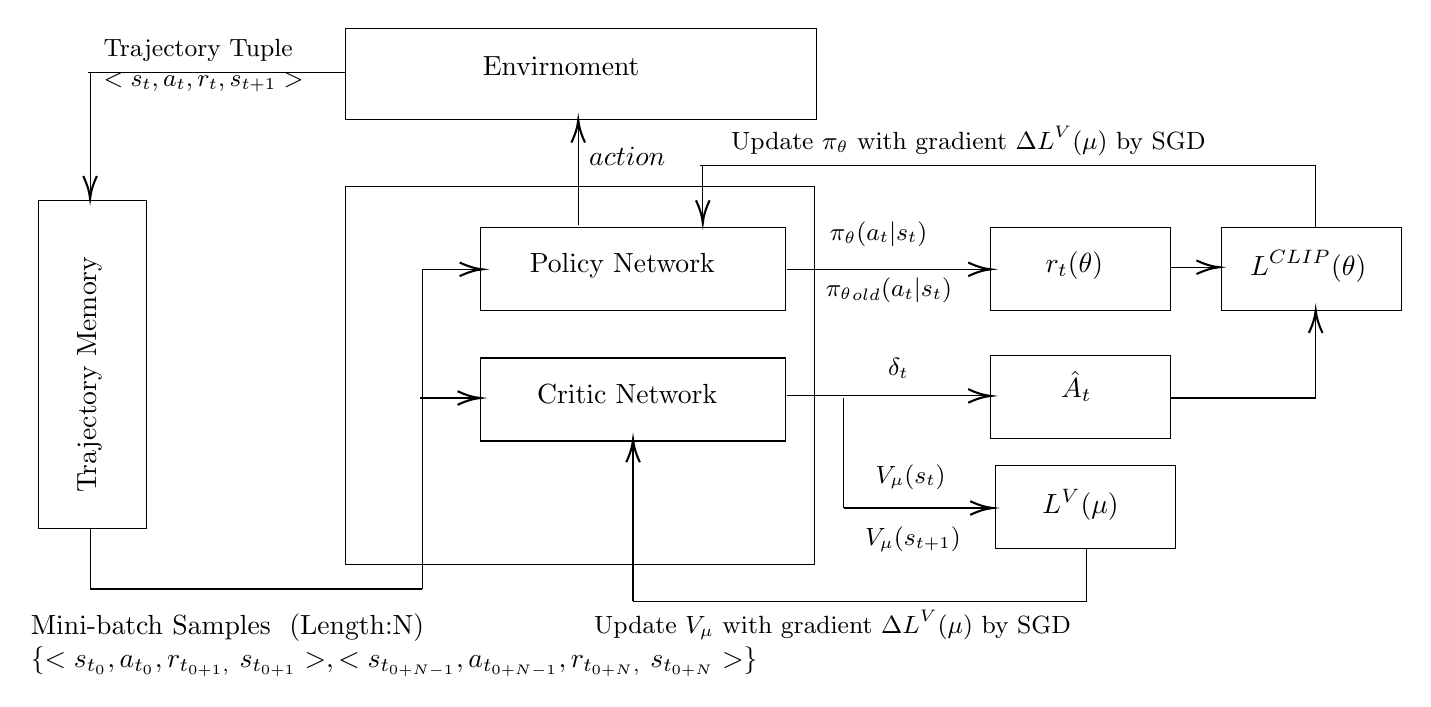
\begin{tikzpicture}[x=0.75pt,y=0.75pt,yscale=-1,xscale=1]
%uncomment if require: \path (0,338); %set diagram left start at 0, and has height of 338

%Shape: Rectangle [id:dp9978943115484824] 
\draw   (26.8,246.3) -- (26.8,88.3) -- (78.8,88.3) -- (78.8,246.3) -- cycle ;

%Shape: Rectangle [id:dp05267034608632715] 
\draw   (174.8,5.14) -- (401.8,5.14) -- (401.8,49.3) -- (174.8,49.3) -- cycle ;
%Shape: Rectangle [id:dp04578612721398789] 
\draw   (174.8,81.3) -- (400.8,81.3) -- (400.8,263.3) -- (174.8,263.3) -- cycle ;
%Shape: Rectangle [id:dp479111495997272] 
\draw   (240,101) -- (386.8,101) -- (386.8,141) -- (240,141) -- cycle ;

%Shape: Rectangle [id:dp3592684590066768] 
\draw   (240,164) -- (386.8,164) -- (386.8,204) -- (240,204) -- cycle ;

%Shape: Rectangle [id:dp5726876145364976] 
\draw   (485.5,101) -- (572.3,101) -- (572.3,141) -- (485.5,141) -- cycle ;

%Shape: Rectangle [id:dp8126568031433179] 
\draw   (597,101) -- (683.8,101) -- (683.8,141) -- (597,141) -- cycle ;

%Shape: Rectangle [id:dp24057721244799102] 
\draw   (488,216) -- (574.8,216) -- (574.8,256) -- (488,256) -- cycle ;

%Shape: Rectangle [id:dp21651348351379074] 
\draw   (485.5,163) -- (572.3,163) -- (572.3,203) -- (485.5,203) -- cycle ;

%Straight Lines [id:da2065459425933598] 
\draw    (313.4,281.3) -- (313.4,205.3) ;
\draw [shift={(313.4,203.3)}, rotate = 450] [color={rgb, 255:red, 0; green, 0; blue, 0 }  ][line width=0.75]    (10.93,-3.29) .. controls (6.95,-1.4) and (3.31,-0.3) .. (0,0) .. controls (3.31,0.3) and (6.95,1.4) .. (10.93,3.29)   ;
%Straight Lines [id:da5843246843678724] 
\draw    (387.8,182.3) -- (483.8,182.3) ;
\draw [shift={(485.8,182.3)}, rotate = 180] [color={rgb, 255:red, 0; green, 0; blue, 0 }  ][line width=0.75]    (10.93,-3.29) .. controls (6.95,-1.4) and (3.31,-0.3) .. (0,0) .. controls (3.31,0.3) and (6.95,1.4) .. (10.93,3.29)   ;
%Straight Lines [id:da5820279370707651] 
\draw    (387.8,121.3) -- (483.8,121.3) ;
\draw [shift={(485.8,121.3)}, rotate = 180] [color={rgb, 255:red, 0; green, 0; blue, 0 }  ][line width=0.75]    (10.93,-3.29) .. controls (6.95,-1.4) and (3.31,-0.3) .. (0,0) .. controls (3.31,0.3) and (6.95,1.4) .. (10.93,3.29)   ;
%Straight Lines [id:da03477812258414015] 
\draw    (414.8,236.3) -- (484.8,236.3) ;
\draw [shift={(486.8,236.3)}, rotate = 180] [color={rgb, 255:red, 0; green, 0; blue, 0 }  ][line width=0.75]    (10.93,-3.29) .. controls (6.95,-1.4) and (3.31,-0.3) .. (0,0) .. controls (3.31,0.3) and (6.95,1.4) .. (10.93,3.29)   ;
%Straight Lines [id:da09026891505962009] 
\draw    (414.8,183.3) -- (414.8,236.3) ;
%Shape: Right Angle [id:dp09688091613107686] 
\draw   (531.8,256) -- (531.8,281.3) -- (313.4,281.3) ;
%Straight Lines [id:da10002566422487891] 
\draw    (51.8,26.3) -- (51.8,85.3) ;
\draw [shift={(51.8,87.3)}, rotate = 270] [color={rgb, 255:red, 0; green, 0; blue, 0 }  ][line width=0.75]    (10.93,-3.29) .. controls (6.95,-1.4) and (3.31,-0.3) .. (0,0) .. controls (3.31,0.3) and (6.95,1.4) .. (10.93,3.29)   ;
%Straight Lines [id:da14348663665795947] 
\draw    (210.8,183.3) -- (237.8,183.3) ;
\draw [shift={(239.8,183.3)}, rotate = 180] [color={rgb, 255:red, 0; green, 0; blue, 0 }  ][line width=0.75]    (10.93,-3.29) .. controls (6.95,-1.4) and (3.31,-0.3) .. (0,0) .. controls (3.31,0.3) and (6.95,1.4) .. (10.93,3.29)   ;
%Straight Lines [id:da1581117014190938] 
\draw    (211.8,121.3) -- (238.8,121.3) ;
\draw [shift={(240.8,121.3)}, rotate = 180] [color={rgb, 255:red, 0; green, 0; blue, 0 }  ][line width=0.75]    (10.93,-3.29) .. controls (6.95,-1.4) and (3.31,-0.3) .. (0,0) .. controls (3.31,0.3) and (6.95,1.4) .. (10.93,3.29)   ;
%Straight Lines [id:da3327122153372011] 
\draw    (211.8,121.3) -- (211.8,275.3) ;
%Shape: Right Angle [id:dp7457457500271234] 
\draw   (211.8,275.3) -- (51.8,275.3) -- (51.8,246) ;
%Straight Lines [id:da24558256059318717] 
\draw    (174.8,26.3) -- (50.8,26.3) ;
%Straight Lines [id:da1907077659365608] 
\draw    (287,100) -- (287,51.3) ;
\draw [shift={(287,49.3)}, rotate = 450] [color={rgb, 255:red, 0; green, 0; blue, 0 }  ][line width=0.75]    (10.93,-3.29) .. controls (6.95,-1.4) and (3.31,-0.3) .. (0,0) .. controls (3.31,0.3) and (6.95,1.4) .. (10.93,3.29)   ;
%Straight Lines [id:da25181356746653694] 
\draw    (347,71.3) -- (347,97) ;
\draw [shift={(347,99)}, rotate = 270] [color={rgb, 255:red, 0; green, 0; blue, 0 }  ][line width=0.75]    (10.93,-3.29) .. controls (6.95,-1.4) and (3.31,-0.3) .. (0,0) .. controls (3.31,0.3) and (6.95,1.4) .. (10.93,3.29)   ;
%Shape: Right Angle [id:dp9296457308111634] 
\draw   (345.8,71.3) -- (642.3,71.3) -- (642.3,101) ;
%Straight Lines [id:da7729636916978786] 
\draw    (642.3,183.3) -- (642.3,143) ;
\draw [shift={(642.3,141)}, rotate = 450] [color={rgb, 255:red, 0; green, 0; blue, 0 }  ][line width=0.75]    (10.93,-3.29) .. controls (6.95,-1.4) and (3.31,-0.3) .. (0,0) .. controls (3.31,0.3) and (6.95,1.4) .. (10.93,3.29)   ;
%Straight Lines [id:da8163897958062174] 
\draw    (572.8,183.3) -- (642.3,183.3) ;
%Straight Lines [id:da9600198123912971] 
\draw    (572.8,120.3) -- (593.8,120.3) ;
\draw [shift={(595.8,120.3)}, rotate = 180] [color={rgb, 255:red, 0; green, 0; blue, 0 }  ][line width=0.75]    (10.93,-3.29) .. controls (6.95,-1.4) and (3.31,-0.3) .. (0,0) .. controls (3.31,0.3) and (6.95,1.4) .. (10.93,3.29)   ;


% Text Node
\draw (44.3,230.3) node [anchor=north west][inner sep=0.75pt]  [rotate=-270] [align=left] {Trajectory Memory};
% Text Node
\draw (509.4,226) node [anchor=north west][inner sep=0.75pt]   [align=left] {$\displaystyle L^{V}( \mu )$};
% Text Node
\draw (518.4,169) node [anchor=north west][inner sep=0.75pt]   [align=left] {$\displaystyle \hat{A}_{t}$};
% Text Node
\draw (510.9,111.5) node [anchor=north west][inner sep=0.75pt]   [align=left] {$\displaystyle r_{t}( \theta )$};
% Text Node
\draw (609.4,111) node [anchor=north west][inner sep=0.75pt]   [align=left] {$\displaystyle L^{CLIP}( \theta )$};
% Text Node
\draw (265.9,175.5) node [anchor=north west][inner sep=0.75pt]   [align=left] {Critic Network};
% Text Node
\draw (262.4,112.5) node [anchor=north west][inner sep=0.75pt]   [align=left] {Policy Network};
% Text Node
\draw (239.8,17.65) node [anchor=north west][inner sep=0.75pt]   [align=left] {Envirnoment};
% Text Node
\draw (407,97) node [anchor=north west][inner sep=0.75pt]  [font=\small] [align=left] {$\displaystyle \pi _{\theta }( a_{t} |s_{t})$};
% Text Node
\draw (405,124) node [anchor=north west][inner sep=0.75pt]  [font=\small] [align=left] {$\displaystyle {\pi _{\theta }}_{old}( a_{t} |s_{t})$};
% Text Node
\draw (435,163) node [anchor=north west][inner sep=0.75pt]  [font=\small] [align=left] {$\displaystyle \delta _{t}$};
% Text Node
\draw (429,214) node [anchor=north west][inner sep=0.75pt]  [font=\small] [align=left] {$\displaystyle V_{\mu }( s_{t})$};
% Text Node
\draw (424,244) node [anchor=north west][inner sep=0.75pt]  [font=\small] [align=left] {$\displaystyle V_{\mu }( s_{t+1})$};
% Text Node
\draw (57,9) node [anchor=north west][inner sep=0.75pt]  [font=\small] [align=left] {Trajectory Tuple\\$\displaystyle < s_{t} ,a_{t} ,r_{t} ,s_{t+1}  >$};
% Text Node
\draw (22,286) node [anchor=north west][inner sep=0.75pt]   [align=left] {Mini-batch Samples \ (Length:N)\\$\displaystyle \{< s_{t_{0}} ,a_{t_{0}} ,r_{t_{0+1} ,\ } s_{t_{0+1}}  >,\dotsc < s_{t_{0+N-1}} ,a_{t_{0+N-1}} ,r_{t_{0+N} ,\ } s_{t_{0+N}}  >\}$};
% Text Node
\draw (293.4,284.3) node [anchor=north west][inner sep=0.75pt]  [font=\small] [align=left] {Update $\displaystyle V_{\mu }$ with gradient $\displaystyle \Delta L^{V}( \mu )$ by SGD};
% Text Node
\draw (359.4,51) node [anchor=north west][inner sep=0.75pt]  [font=\small] [align=left] {Update $\displaystyle \pi _{\theta }$ with gradient $\displaystyle \Delta L^{V}( \mu )$ by SGD};
% Text Node
\draw (291,61.3) node [anchor=north west][inner sep=0.75pt]   [align=left] {$\displaystyle action$};


\end{tikzpicture}}
    \caption{Flowchart of actor critic based PPO learning model \cite{LimHun_ppo_flowchart}}
    \label{fig:ppo_flowchart}
\end{figure}

\begin{table}[H]
\centering
        
\begin{tabular}{p{0.75\textwidth}|p{0.1\textwidth}}
\toprule
 Hyper-parameter & Value \\
\midrule
 Clipping parameter ($\displaystyle \epsilon $) & 0.2 \\
\hline 
 Optimization algorithm & Adam \\
\hline 
 Learning rate ($\displaystyle \eta _{\mu } ,\eta _{\theta }$) & 0.0001 \\
\hline 
 Discount factor ($\displaystyle \gamma $) & 0.99 \\
\hline 
 The number of steps to run for each environment per update & 1000 \\
\hline 
 Entropy coefficient for the loss calculation & 0.01 \\
\hline 
 Number of training mini batches per update & 4 \\
 \bottomrule
\end{tabular}
\caption{PPO Algorithm Hyper-parameter configuration}
\label{tbl_hyperparam_PPO}
\end{table}

\noindent After pre training, model is trained for $16 \cdotp 10^6$ time steps with 1000 steps per episode using PPO algorithm. \autoref{fig:PPO_LOG_16M} shows reward per episode and rolling average. Notice how model learned within 5000 episodes, and later reward is saturated within 500 to 600.
\begin{figure}[H]
    \centering
    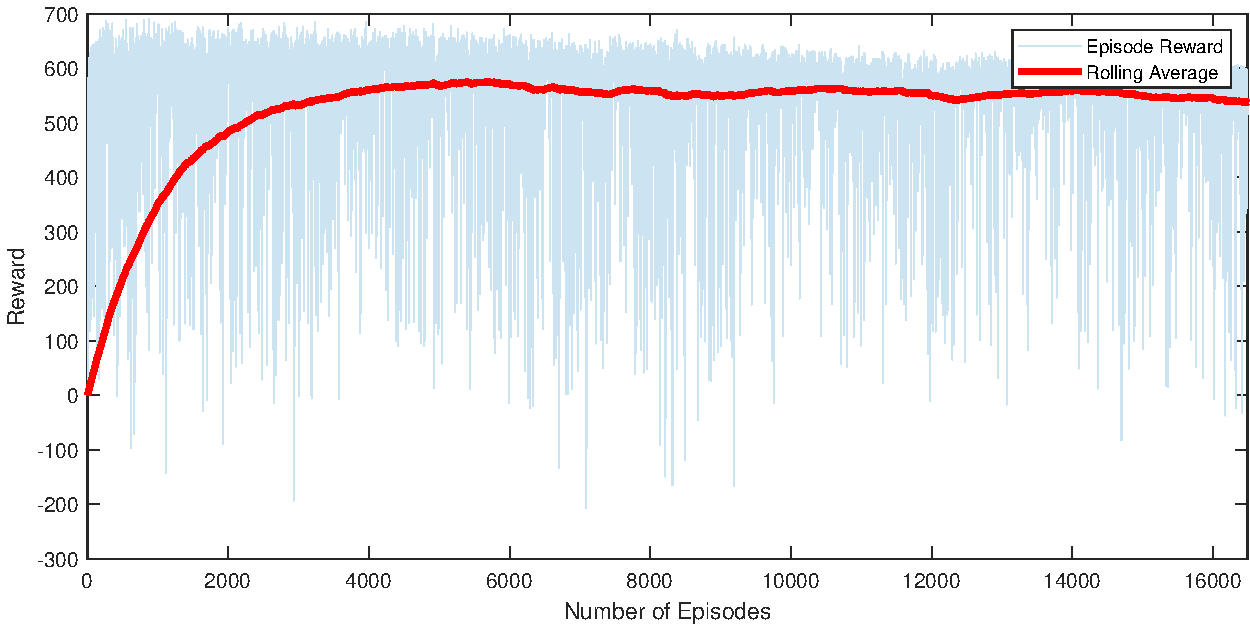
\includegraphics[width=\textwidth]{figures/plots/RL/PPOlog16M.pdf}
    \caption{Averaged episode reward for 16000 episodes of PPO training}
    \label{fig:PPO_LOG_16M}
\end{figure}
\subsection{Test Results}
Let us consider a test case, Neural Network based steering has to cancel attitude error in terms of Euler angles $\displaystyle \phi ,\theta ,\psi =[ -179\ ,\ -37,\ \ 140] \ \deg$ considering initial and final state shown in \autoref{tbl:nn_vscmg_states}
\begin{table}[H]
        \centering
        
\begin{tabular}{p{0.16\textwidth}|p{0.50\textwidth}|p{0.2\textwidth}}
\toprule 
 Parameter & Value & Unit \\
\midrule 
 $\displaystyle q$ & $\displaystyle [ 0.3036\ \ \ \ 0.3228\ \ \ -0.8891\ \ \ -0.1146]^{T}$ & - \\
\hline 
 $\displaystyle \omega $ & $\displaystyle [ 0\ 0\ 0]^{T}$ & $\displaystyle \deg /\sec$ \\
\hline 
 $\displaystyle q_{d}$ & $\displaystyle [ 1\ 0\ 0\ 0]^{T}$ & - \\
\hline 
 $\displaystyle \omega _{d}$ & $\displaystyle [ 0\ 0\ 0]^{T}$ & $\displaystyle rad/\sec$ \\
\hline 
 $\displaystyle \delta $ & $\displaystyle [ -0.7729\ \ \ \ 1.2424\ \ \ \ 0.6058\ \ \ \ 2.6412]^{T}$ & $\displaystyle rad$ \\
\hline 
 $\displaystyle \Omega $ & $\displaystyle [ 0\ 0\ 0\ 0]^{T}$ & $\displaystyle rad/\sec$ \\
 \bottomrule
\end{tabular}
        \caption{Initial and desired states for Attitude error tracking with Neural Network based VSCMG steering Law }
        \label{tbl:nn_vscmg_states}
        \end{table}
\noindent Results of error canceling maneuver using Neural network based steering are in \autoref{fig:nn__Torque_1} to \autoref{fig:nn__Omega_dot}. Being long slew maneuver, initial attitude error was large as consequence large demand torque variation can seen in first few seconds although after 10 seconds.
\begin{figure}[H]
    \centering
    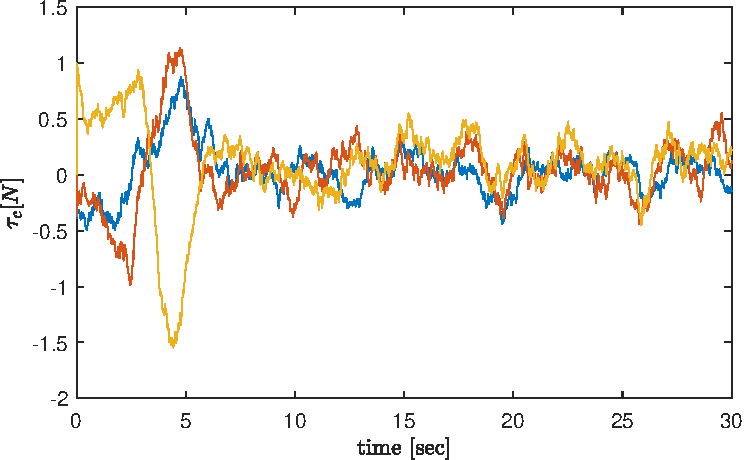
\includegraphics[width=\textwidth]{figures/plots/RL/nn_Torque.pdf}
    \caption{NN based steering: Required torques}
    \label{fig:nn__Torque_1}
\end{figure}
\noindent Variations in reaction wheels spins are more than that compared to gimbal angles, hence we can infer neural network has prioritized RWs over CMGs for this maneuver.
\begin{figure}[H]
    \centering
    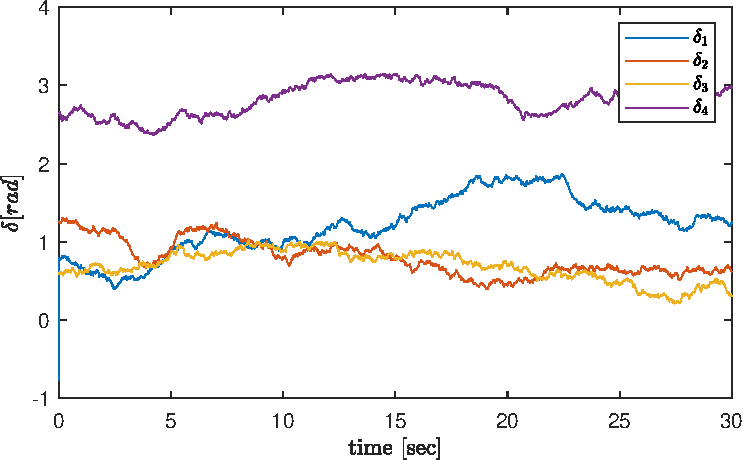
\includegraphics[width=\textwidth]{figures/plots/RL/nn_delta.pdf}
    \caption{NN based steering: Gimbal angles}
    \label{fig:nn__delta}
\end{figure}
\begin{figure}[H]
    \centering
    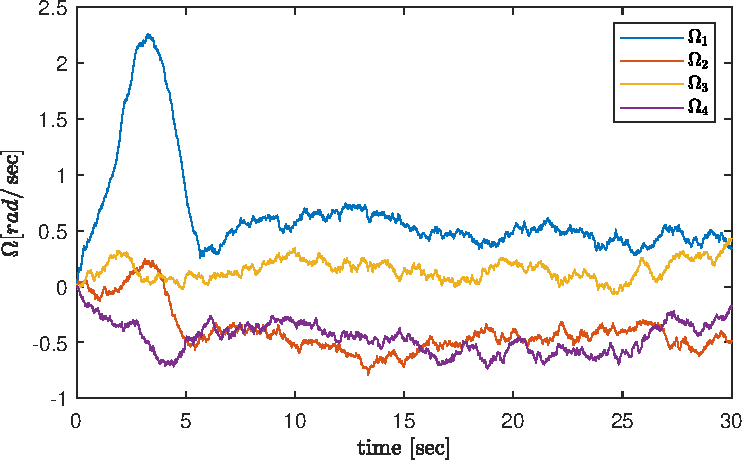
\includegraphics[width=\textwidth]{figures/plots/RL/nn_Omega.pdf}
    \caption{NN based steering: RW velocities}
    \label{fig:nn__Omega}
\end{figure}

\begin{figure}[H]
    \centering
    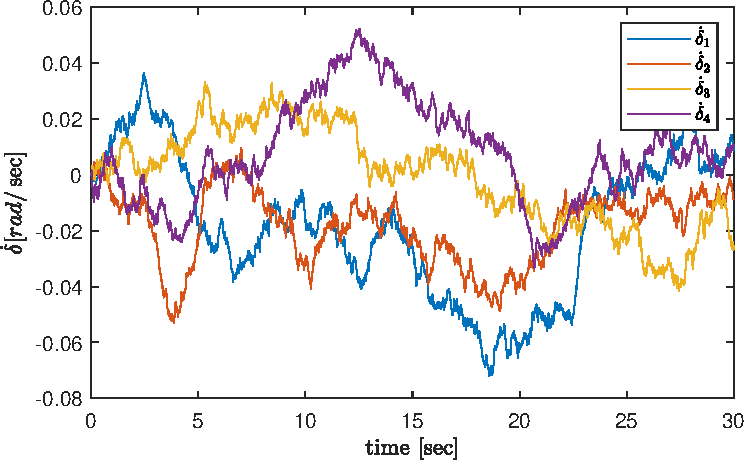
\includegraphics[width=\textwidth]{figures/plots/RL/nn_Delta_dot.pdf}
    \caption{NN based steering: Gimbal Velocities}
    \label{fig:nn__Delta_dot}
\end{figure}
\noindent \autoref{fig:nn__Delta_dot} and \autoref{fig:nn__Omega_dot} are control action performed by agent. Notice order of magnitude of RW accelerations and gimbal velocities are within permissible range and no large variation occurred.
\begin{figure}[H]
    \centering
    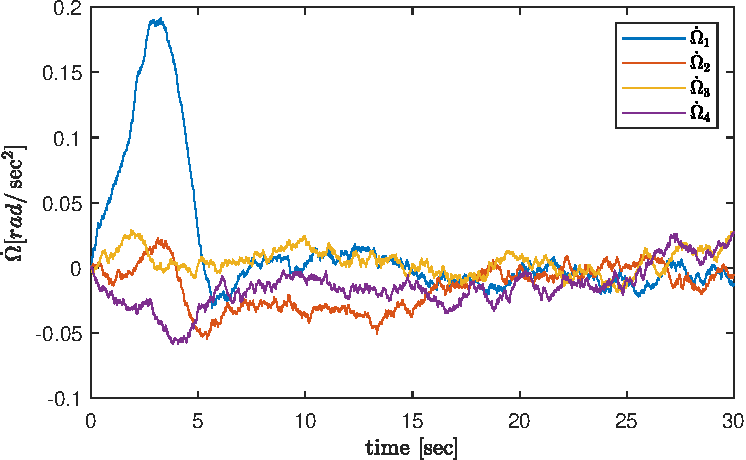
\includegraphics[width=\textwidth]{figures/plots/RL/nn_Omega_dot.pdf}
    \caption{NN based steering: RW Accerlations}
    \label{fig:nn__Omega_dot}
\end{figure}
\noindent Output data of neural network can be amplified or attenuated based on steady state requirements, moreover different activation functions at output layer can be used. A GUI based script is developed in order to monitor states and 3d visualization of VSCMG. Screenshot of testing trained PPO model is shown in \autoref{fig:model_explorer}. Main advantage of script is along with plots, attitude command and other model related parameters can be updated in real time, giving user an option for better calibrating the ACS according to required performance. 
\begin{figure}[H]
    \centering
    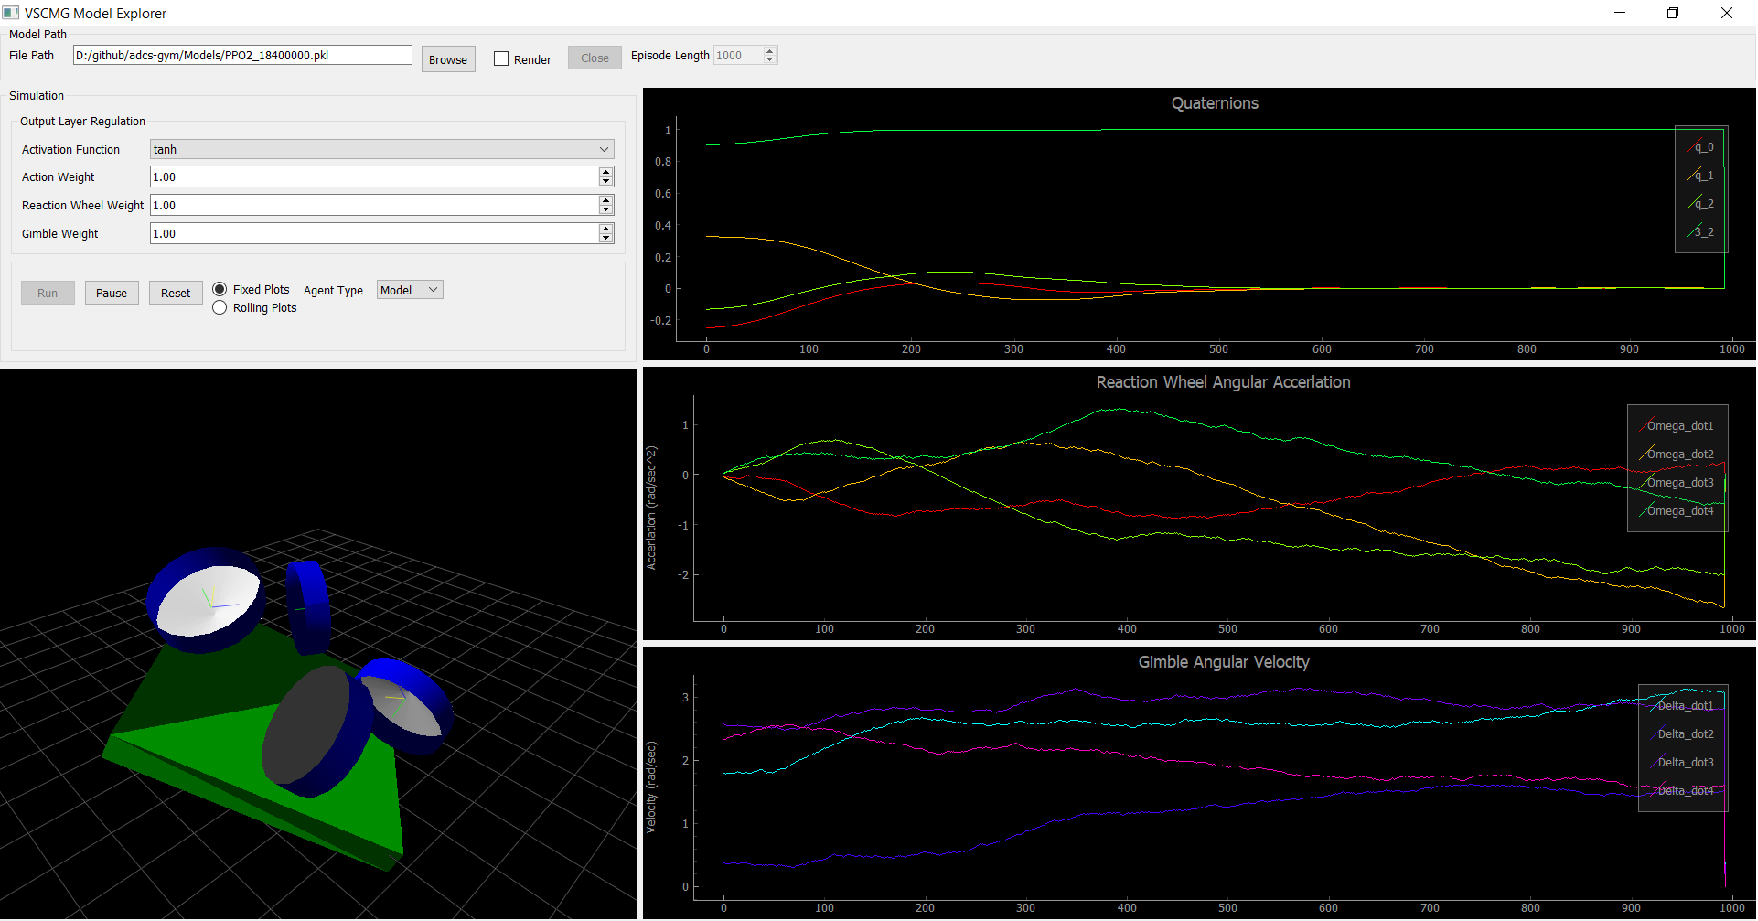
\includegraphics[width=\textwidth]{figures/AI/ModelExplorer1.pdf}
    \caption{VSCMG Model and expert agent Testing GUI}
    \label{fig:model_explorer}
\end{figure}


\section{Comparison of Neural Network and SR-VSCMG Steering Law}
\newacronym{sr-vscmg}{SR-VSCMG}{Singularity-Robust VSCMG Steering Law}
Following discussion assumes regulation maneuver with initial attitude error of $90^\circ$ in yaw angle has to be canceled. In order to evaluate the performance of steering law, spacecraft actuators are deliberately kept in singular states as shown in  \autoref{tbl:nnvscmg_params}. Notice angular momentum of all reaction wheels is zero, moreover required torque is orthogonal to CMG torque axis. 
\begin{table}[ht]
        \centering
\begin{tabular}{|p{0.2\textwidth}|p{0.4\textwidth}|p{0.3\textwidth}|}
\hline 
 Parameter & Value & Unit \\
\hline 
 $\displaystyle q$ & $\displaystyle [ 1\ 0\ 0\ 0]^{T}$ & - \\
\hline 
 $\displaystyle q_{d}$ & $\displaystyle [ 0.7071\ 0\ 0\ 0.7071]$ & - \\
\hline 
 $\displaystyle \omega _{d}$ & $\displaystyle [ 0\ 0\ 0]^{T}$ & $\displaystyle rad/\sec$ \\
\hline 
 $\displaystyle \delta $ & $\displaystyle [ 0,\ 0,\ 0,0]^{T}$ & $\displaystyle rad$ \\
\hline 
 $\displaystyle \Omega $ & $\displaystyle [ 0,\ 0,\ 0,\ 0]^{T}$ & $\displaystyle rad/\sec$ \\
\hline 
 $\displaystyle K_{w}$ & 4.4 & - \\
\hline 
 $\displaystyle K_{q}$ & 10.1 & - \\
 \hline
\end{tabular}
        \caption{Simulation parameters for regulation maneuver in order to cancel attitude error of $\displaystyle 90^{\circ }$ in yaw angle.}
        \label{tbl:nnvscmg_params}
        \end{table}
        
\noindent Results of Neural Network based and \acrfull{sr-vscmg} are concurrently simulated using specially developed Model Explorer software \autoref{fig:model_explorer} discussed in earlier section. Quaternions of simulation with neural network based steering are shown in \autoref{fig:nn_q} and \acrlong{sr-vscmg} shown in \autoref{fig:vs_q}. Notice that with NN based steering quickly approaches desired state within 5 seconds but a small steady state error persists, whereas with \acrshort{sr-vscmg} steering, slight overshoot is seen followed by long period osculation near desired state. Notice that with same control gains NN based steering quickly stabilizes and follows different trajectory than \acrshort{sr-vscmg} steering law. As shown in \autoref{fig:nnvscmg_w} small variation in body rates are visible in other two axis since NN based steering is following slightly different trajectory than SR-VSCMG for which variation in body rate is only along yaw axis. Even after approaching close to desired state small but significant amount of variations are persistent in all three body rates.
\begin{figure}[ht]
     \centering
     \begin{subfigure}[b]{0.49\textwidth}
         \centering
         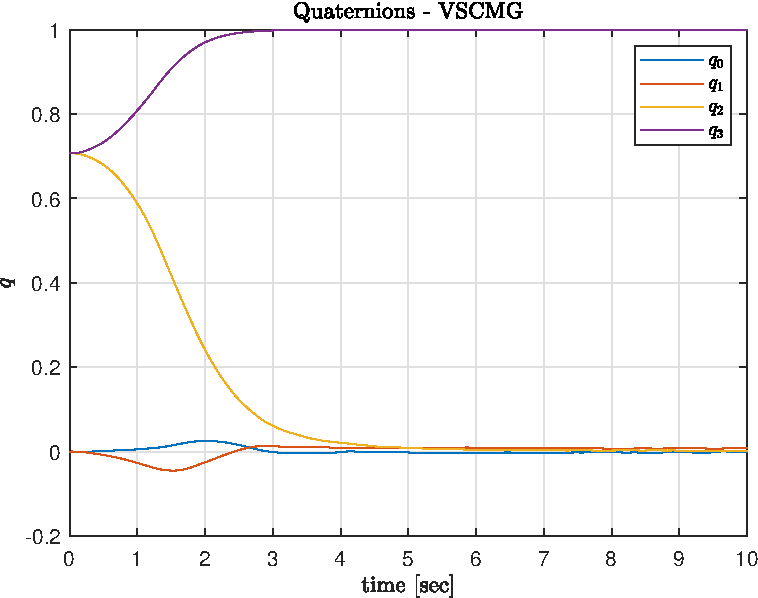
\includegraphics[width=\textwidth]{figures/plots/Results/vs-nn-q.pdf}
         \caption{}
         \label{fig:nn_q}
     \end{subfigure}
     \begin{subfigure}[b]{0.49\textwidth}
         \centering
         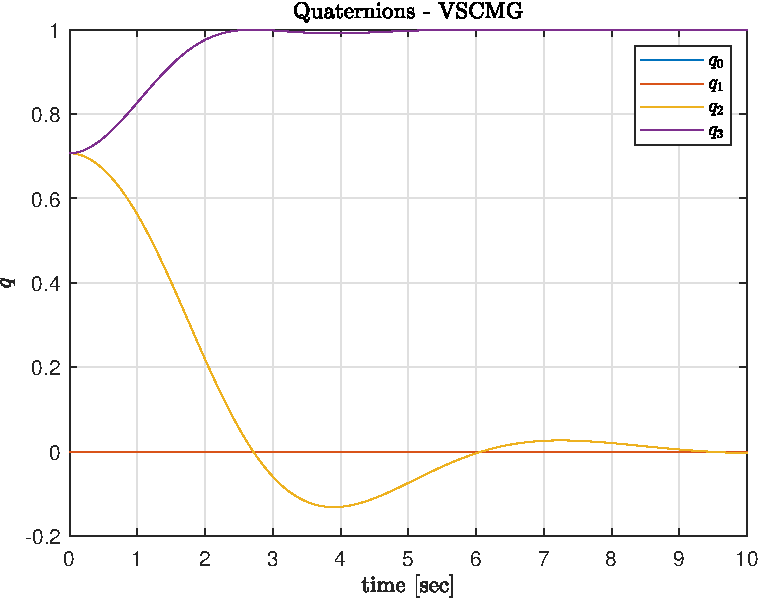
\includegraphics[width=\textwidth]{figures/plots/Results/vs-vs-q.pdf}
         \caption{}
         \label{fig:vs_q}
     \end{subfigure}
        \caption{Attitude quaternions : (a) Neural Network based steering (b) SR-VSCMG steering}
        \label{fig:nnvscmg_q}
\end{figure}

\begin{figure}[ht]
     \centering
     \begin{subfigure}[b]{0.49\textwidth}
         \centering
         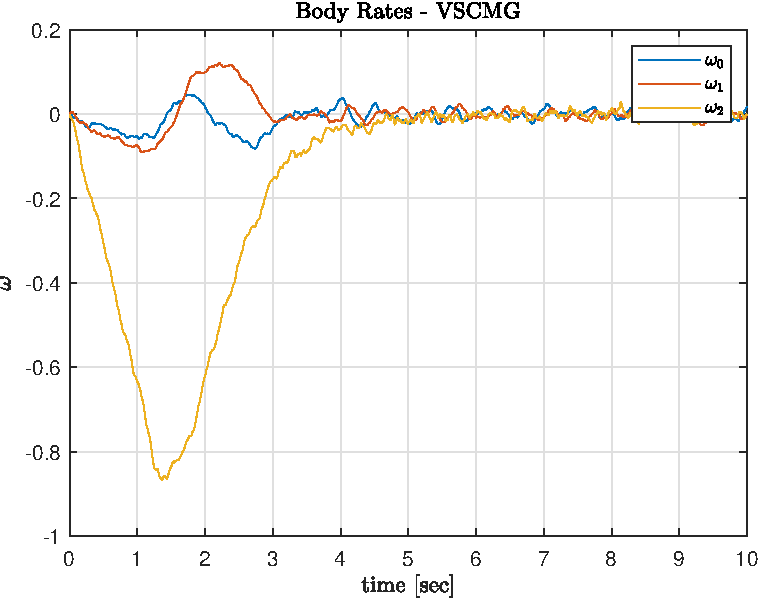
\includegraphics[width=\textwidth,trim={0 0 0 0.35cm},clip]{figures/plots/Results/vs-nn-w.pdf}
         \label{fig:nn_w}
     \end{subfigure}
     \begin{subfigure}[b]{0.49\textwidth}
         \centering
         \includegraphics[width=\textwidth,trim={0 0 0 0.35cm},clip]{figures/plots/Results/vs-vs-w.pdf}
         \label{fig:vs_w}
     \end{subfigure}
        \caption{Body rates (rad/sec): (a) Neural Network based steering (b) SR-VSCMG steering}
        \label{fig:nnvscmg_w}
\end{figure}

\begin{figure}[ht]
     \centering
     \begin{subfigure}[b]{0.49\textwidth}
         \centering
         \includegraphics[width=\textwidth,trim={0 0 0 0.35cm},clip]{figures/plots/Results/vs-nn-Omg.pdf}
          \caption{}
         \label{fig:nn_Omg}
     \end{subfigure}
     \begin{subfigure}[b]{0.49\textwidth}
         \centering
         \includegraphics[width=\textwidth,trim={0 0 0 0.35cm},clip]{figures/plots/Results/vs-vs-Omg.pdf}
          \caption{}
         \label{fig:vs_Omg}
     \end{subfigure}
     
        \caption{Reaction wheel angular velocity : (a) Neural Network based steering (b) SR-VSCMG steering}
        \label{fig:nnvscmg_Omg}
\end{figure}

\begin{figure}[ht]
     \centering
     \begin{subfigure}[b]{0.49\textwidth}
         \centering
         \includegraphics[width=\textwidth]{figures/plots/Results/vs-nn-delta.pdf}
          \caption{}
         \label{fig:nn_delta}
     \end{subfigure}
     \begin{subfigure}[b]{0.49\textwidth}
         \centering
         \includegraphics[width=\textwidth]{figures/plots/Results/vs-vs-delta.pdf}
          \caption{}
         \label{fig:vs_delta}
     \end{subfigure}
     
        \caption{Gimbal Angle : (a) Neural Network based steering (b) SR-VSCMG steering}
        \label{fig:nnvscmg_delta}
\end{figure}


\noindent Each reaction wheel wheel is running at slightly different angular velocity in case of NN based steering, in fact this is the reason we can observe slightly different path followed than shortest path as in case of SR-VSCMG steering.
Most significant difference is  seen in Gimbal Angles, comparison is shown in \autoref{fig:nnvscmg_delta}. Very high frequency jitter is clearly visible in \autoref{vs_delta} since CMGs are very close to singularity, whereas in the case of \autoref{fig:nn_delta} even in the proximity of singularity no high frequency contents are visible. Considering structural integrity of system Neural network based steering performs better near singular state.
\autoref{fig:nnvscmg_sings} depicts three types of singularities. System becomes singular in case of rank deficiency that is transformation matrix is no longer full rank and hence non invertible. Degree or closeness to singularity can be measured with taking determinant of matrix. Here CMG singularity measure $m_c = \det(CC^T)$, Reaction wheel singularity measure measure $m_s = \det(DD^T)$ and complete VSCMG singularity measure measure $m_{vscmg} = \det(QQ^T)$ is shown in \autoref{fig:nnvscmg_sings}. CMGs are in singular state at the beginning since all reaction wheels are at rest. As angular momentum of RW is increased CMGs are getting away from singular state. Notice that in case of NN based steering distance from singularity is much higher at maximum RW angular momentum. Measure of RW remains constant in case of SR-VSCMG steering law since only RWs are used throughout the maneuver and gimbal angle remains constant. Whereas in case of NN-Steering, reaction wheel are moving far away from singularity due to variation in gimbal angle. Another contributing factor for increased in singular distance of RW singularity is different angular momentum of RWs. 

\begin{figure}[ht]
     \centering
     \begin{subfigure}[b]{0.3\textwidth}
         \centering
         \includegraphics[width=\textwidth]{figures/plots/Results/vs-vs-CC.pdf}
        \caption{}
    \label{fig:nnvscmg_CC}
     \end{subfigure}
     \begin{subfigure}[b]{0.3\textwidth}
         \centering
         \includegraphics[width=\textwidth]{figures/plots/Results/vs-vs-DD.pdf}
          \caption{}
        \label{fig:nnvscmg_DD}
     \end{subfigure}
      \begin{subfigure}[b]{0.3\textwidth}
         \centering
         \includegraphics[width=\textwidth]{figures/plots/Results/vs-vs-QQ.pdf}
          \caption{}
        \label{fig:nnvscmg_QQ}
     \end{subfigure}
        \caption{System approaches singular state as singularity measure tends to zero (a) CMG singularity; (b) Reaction Wheel singularity and (c) VSCMG singularity}
        \label{fig:nnvscmg_sings}
\end{figure}

\begin{figure}[ht]
     \centering
     \begin{subfigure}[b]{0.49\textwidth}
         \centering
         \includegraphics[width=\textwidth]{figures/plots/Results/vs-nn-delta.pdf}
          \caption{}
         \label{fig:nn_delta}
     \end{subfigure}
     \begin{subfigure}[b]{0.49\textwidth}
         \centering
         \includegraphics[width=\textwidth]{figures/plots/Results/vs-vs-delta.pdf}
          \caption{}
         \label{fig:vs_delta}
     \end{subfigure}
     
        \caption{CMG gimbal angles : (a) Neural Network based steering (b) SR-VSCMG steering}
        \label{fig:nnvscmg_delta}
\end{figure}
Multiple simulations keeping same scenario are performed considering both NN based and SR-VSCMG based steering law
For above maneuver of 10 seconds, SR-VSCMG based steering law requires average of 3.82 seconds to complete entire simulation whereas neural network based steering requires 2.16 seconds on  intel i7 processor. Processing time is reduced by 1.66 seconds which is clear computational advantage provided by proposed steering law. 
\noindent From above results it is clear that SR-VSCMG steering law provides more precise attitude tracking performance, although Neural network based steering is better at quickly approaching desires state following different trajectory with maintain body in  allowable range.  Most important advantage of proposed technique is seen in proximity of singularity. SR-VSCMG based steering undergoes very high frequency jitter which not favaurable considering structural integrity of spacecraft. NN based steering is inversion free technique thus very large velocities are not present in proximity of singularity. Steady state error and body rate oscillations in proximity of desired state can be reduced by regulating output layer by appropriate activation such as softmax and by filtering the output in order provide smooth actions to actuators. After numerous Monte Carlo simulations it is observed that NN based agent always converges to desired states but may follow trajectories which are not intuitive or similar to SR-VSCMG law. NN performance can be improved by more training and selecting better reward function crafted for required performance. A Hybrid of both steering law can be used, NN based steering for large slew maneuvers when error is large and SR-VSCMG based steering when current state is in proximity of desired state i.e. when error is small.
%\part{Testbed}
% Mechanical Design
\chapter{Mechanical Design}
\label{chap:7}
In this section brief description of VSCMG test-bed mechanical design is described. Various manufacturing techniques has been employed and design choices are made in order to make sure simplicity and keeping overall cost within affordable range. 
\section{System Overview}
\newacronym{sgcmg}{SGCMG}{Single Gimble Control Moment Gyroscope}
Test bed is designed in order to simulate attitude control system of satellite equipped with momentum exchange device. A re-configurable and modular designed is realised so that various arrangements of Reaction Wheel, CMG configurations could be tested with minimum modification. Primary design consist of four \acrshort{sgcmg} units arranged in pyramid configuration on sandwich of two acrylic sheets as main platform to hold entire electronics and power system. This platform is balanced on sharp pin keeping center of gravity of entire unit below but close to pin point. This pin joint allows complete 360 degree of rotation around yaw axis as well as $\pm 60 \deg$ in roll and pitch axis constraining translation motion. Selected degree of freedom is sufficient for most of the GNC verification requirements. Entire assembly is balanced on tip placed on a small custom made tripod, a rendered view of test bed is shown in \ref{fig:my_AssemblyACR}

\begin{figure}[ht]
    \centering
    \includegraphics[width=0.55\textwidth]{figures/Assembly/AssemblyACR - Transperent.pdf}
    \caption{VSCMG Attitude Control System test bed Assembly (Rendered)}
    \label{fig:my_AssemblyACR}
\end{figure}

\section{Reaction Wheel Motor}
\newacronym{bldc}{BLDC}{Brushless DC}
Three phase permanent magnet \acrfull{bldc} outrunner motor is selected for reaction wheel. As name suggest brushless motor does not have brush contact for electric power and needs special commutation sequence in order to properly operate at desired torque and speed explained in next chapter. These are highly efficient and provide greater torques compared to brushed dc motors \cite{bldc}. Outrunner motor has external rotor casing with attached permanent magnets and inner stator with three phase coil winding. Very low cost high RPM and High rotor inertia \acrshort{bldc} motors found shown in \autoref{fig:BLDC2} which can rotate at 900 RPM/Volt and has with inertia $3.140 kg \ mm^2$ evaluated using CAD software. This configuration is suitable for ACS testbench requirements.
\begin{figure}[ht]
    \centering
    \includegraphics[width=0.80\textwidth]{figures/Assembly/BLDC2.pdf}
    \caption{Three phase, outrunner, Brushless DC Motor as reaction wheel}
    \label{fig:BLDC2}
\end{figure}

\section{Gimbal Motor}
From numerical simulations performed in earlier chapters it is noted that gimbal motor speed is relatively very slow hence 4 wire stepper motor is selected as gimbal actuator. As shown \autoref{fig:NEMA17} in Standard NEMA 17HS081004 motor of 20mm length with $1.8 \deg$ step angle \cite{web:ds_nema17} is used due to simplicity of control by using appropriate step sequence and and ability of micro stepping in order to have precise resolution. These type of motors are available in standard form factor and in affordable cost since most of the 3d printers available in market are equipped with such motor. 
\begin{figure}[ht]
    \centering
    \includegraphics[width=0.80\textwidth]{figures/Assembly/NEMA17.pdf}
    \caption{NEMA 17HS081004 Stepper motor \cite{web:ds_nema17}}
    \label{fig:NEMA17}
\end{figure}
\section{Slip Ring}
In order to transfer power from stationary component to rotating component slip ring is used. 6 channel slip ring is used as shown in \autoref{fig:SLP_RNG} it has 6 wires going in to large stationary part with flange and coming out from rotating end. Selected slip ring has 1A nominal current carrying capacity at maximum 300 RPM. One of the most important component needs to taken care of while designing SGCMG assembly.

\begin{figure}[ht]
    \centering
    \includegraphics[width=0.60\textwidth]{figures/Assembly/SLP_RNG.pdf}
    \caption{6 channel Slip Ring}
    \label{fig:SLP_RNG}
\end{figure}


\section{SGCMG Assembly Design}
In order to achieve modular design, an unit of \acrlong{sgcmg} sub assembly is designed. Each SGCMG unit has a reaction wheel motor mounted on a gimbal attached to gimbal motor keeping reaction wheels center of mass in line with gimbal rotation axis. Since gimbal motor may perform multiple revolutions, inner motor which is reaction wheel needs to be powered such a way that power cables should not hinder and entangle due to rotations of outer gimbal motor. For this reason a power wires for reaction wheel motors are passed through slip ring which allows transmission of power supply from stationary to rotating structure. A magnetic encoder is placed behind the gimbal motor in order to have angle and angular velocity feedback from gimbal motor, an SGCMG unit is shown in. Two structural components of \acrshort{sgcmg} fabricated with 3D printing ABS material are:
\begin{itemize}
    \item Gimbal Motor Mount
    \item Reaction Wheel Mount
\end{itemize}
\subsection{Gimbal Motor Mount}
Important structural component of SGCMG is designed to support stepper motor at one end and slip ring at other end. Special attention given so that Reaction wheel mount which would be attached to gimbal motor shaft should have enough clearance to allow free rotation of Reaction Wheel Mount. Power to the reaction wheel is provided through slip ring, hence a provision is made to hold slip ring with it's axis in line with gimbal motor shaft as shown in \autoref{fig:GMBL_MNT}. A slot at the end of mount allows proper placement of magnetic encoder in order to have feedback from stepper motor. A complete standalone SGCMG unit is shown in \autoref{fig:SGCMG_ASM}.

\begin{figure}[ht]
    \centering
    \includegraphics[width=\textwidth]{figures/Assembly/STP_MOUNT.pdf}
    \caption{Gimbal Motor Mount (Rendered)}
    \label{fig:GMBL_MNT}
\end{figure}

\subsection{Reaction Wheel Mount}
C shaped mount is used to hold Reaction Wheel motor as shown in, BLDC motor is mounted on web of C channel. Reaction wheel mount is connected to stepper motor shaft at one end while other end is supported by rotating end of slip ring. Special attention is paid in order to connect \acrshort{bldc} wires from slip ring without hindering any component. 

\begin{figure}[ht]
    \centering
    \includegraphics[width=\textwidth]{figures/Assembly/rwMount.pdf}
    \caption{Reaction Wheel Motor Mount (Rendered)}
    \label{fig:RW_MNT}
\end{figure}

\begin{figure}[ht]
    \centering
    \includegraphics[width=\textwidth]{figures/Assembly/SGCMG.pdf}
    \caption{Complete SGCMG assembly (Rendered)}
    \label{fig:SGCMG_ASM}
\end{figure}

\section{Base Platform}
Central structure of test bed which shall hold together all the SGCMG units, power system and other required electronics components. Base platform consist of two acrylic plates fabricated using laser cutting as per design, sand-witched together using spacers. This type of two layer design incorporated so that most of the electronic components and PCBs can use the place between two plates. Batteries are fixed on bottom plate whereas four SGCMG units are bolted on top plate in order to bring center of mass as close to plates as possible. Entire design is kept symmetric in order to simplify manufacturing but most important mass balancing requirement. Most important requirements is the entire platform needs to be balanced on sharp tip with it's center of mass below but closer to tip. Since there will be uncertainties in mass distribution due to the fact presence of wiring and other non modeled components we can not guaranty that CoM is at desired location. Hence a threaded Allen bolt with sharp tip is used. A 3D printed pyramid structure is mounted on top base plate. This part has threaded hole at the center in order to hold sharp cone pointed bolt. This sub assembly shown in \autoref{fig:PLATFORM_TIP_ASM} allows variable position of pivot so that distance of center of mass from pivot along z axis can be shifted as per requirement. A small 3D printed tripod is designed on which entire base platform shall be balanced. Due to the fact that sharp tip may easily damage 3D printed structure, a steal coin is fixed on the top of tripod shaft and entire satellite platform will rest on this steel coin at the edge of tip.

\begin{figure}[ht]
    \centering
    \includegraphics[width=\textwidth]{figures/Assembly/SGCMG.pdf}
    \caption{Sharp tip mounting assembly employed to minimize rotational friction with 360 degree rotational freedom in yaw axis and $\pm 60 \deg$ allowed rotation in roll and pitch axis}
    \label{fig:PLATFORM_TIP_ASM}
\end{figure}

% Electrical Design
\chapter{Electronics Design}
\label{chap:8}
Wiring diagrams, communications, embedded system...
ESP32, ESP8266, ESC, Stepper Driver, AMS5600 Batteries, Power Supply... 
\begin{comment}


\section{Special commands provided by \textsf{sapthesis}}

\textsf{Sapthesis} provides some special commands, particularly useful for scientific works. You can use for example the roman shape, instead of the italic, for the imaginary unit (\texttt{\bs iu}) and Napier's number (\texttt{\bs eu}):
\begin{equation}
\eu^{\iu\pi}+1=0
\end{equation}

There are also two commands to speed up the writing of derivatives. In the following example we have used the commands \texttt{\bs der} and \texttt{\bs pder}):
\begin{equation}
\der{f}{x} \qquad \pder[2]{f}{y}
\end{equation}


\textsf{Sapthesis} provides also 4 commands to improve the writing of subscripts, \texttt{\bs rb} and \texttt{\bs tb}, and superscripts, \texttt{\bs rp} and \texttt{\bs tp}. Two of these commands, \texttt{\bs rb} and \texttt{\bs rp}, can be used both in text and in math mode and compose their argument in roman. The other two, \texttt{\bs tb} and \texttt{\bs tp}, can be used only in text mode and compose their argument as are. Here it is an usage example of \texttt{\bs rb} and \texttt{\bs rp}:
\[
a_b \neq a\rb{b}\qquad a^b \neq a\rp{b}
\]
And here it is an usage example of \texttt{\bs tb}: \emph{Cu\tb{It} indicates copper bought in Italy}. And a usage example of \texttt{\bs ts}: \emph{Cher G\tp{le} Napol\'eon}.


Then several commands for the correct typesetting of unit of measurements are provided. For example the command \texttt{\bs un} typesets its argument in roman and leaves a thin space between the number and the unit: $25\un{m}$, $3.5\un{m/s}$. Other commands are: (\texttt{\bs g}) 45\g, (\texttt{\bs C}) 30\,\C, (\texttt{\bs A}) 12\,\A, (\texttt{\bs micro}) 40\,\micro m, (\texttt{\bs ohm}) 27\,\ohm. 

We have also \texttt{\bs x} as abbreviation of \texttt{\bs times}: \$7 \bs x 10\^{}5\$ gives $7 \x 10^5$. Then \texttt{\bs di} is the differential symbol which automatically insert the correct spacing.
\[
\int x \di x
\]

Finally we have defined the color \textsf{sapred} which is the official color
of Sapienza -- University of Rome. It is defined as RGB(130,36,51). \textcolor{sapred}{This text is written with the color \textsf{sapred}.}
\marginpar{This is a fancy margin note!}
In the following dummy text you can observe the usage of \texttt{\bs mnote} command which typesets fancy margin notes.\cite{Baker2016}
\end{comment}

% Hardware in Loop Simulations
\chapter{Hardware in Loop Simulations}
\label{chap:9}
Real time simulations of VSCMG testbed are discussed in this chapter. 
Various investigations are performed on prototype in order to verify control law and tweak the model dynamics, since exact dynamics of commercial off the shelf affordable components used to build the prototype were unknown. However after several experimental tests so that system works properly as per requirements. Test data is recorded in real time and results are exported to Matlab for post processing.
\section{Free Motion (ACS off)}
Platform kept placed on custom made tripod is balancing on sharp tip, this imitates free attitude motion. A theoretical point contact has three degree of freedom in attitude and constrained in translation motion. If point of contact coincides with the center of mass of platform a free attitude simulation can be achieved. Although practically achieving zero friction motion is impossible with this method due to geometrical constraints and difficulty of mass balancing. Considering these problems center of mass is kept below point of contact thus platform imitates as physical pendulum. Behaviour of test-setup with initial disturbance and no active control system is shown in \autoref{fig:free-w1} and \autoref{fig:free-eul1}. Platform is subjected to two conservative disturbances, first near $5 \sec$ and damps after $40 \sec$. And after second disturbance, amplitude of angular velocity peaks keeps decreasing and completely fade away after 50 seconds mainly due to friction in sharp tip and stand.

%\begin{figure}[ht]
%    \centering
%    \includegraphics[width=1.0\textwidth]{figures/plots/exp/free-q1.pdf}
%    \caption{}
%    \label{fig:free-q1}
%\end{figure}

\begin{figure}[ht]
    \centering
    \includegraphics[width=0.7\textwidth]{figures/plots/exp/free-w1.pdf}
    \caption{ACS off free motion of test bed upon disturbance}
    \label{fig:free-w1}
\end{figure}

\begin{figure}[ht]
    \centering
    \includegraphics[width=0.7\textwidth]{figures/plots/exp/free-eul1.pdf}
    \caption{Free response of platform subjected to disturbance, Euler angles ($\deg$)}
    \label{fig:free-eul1}
\end{figure}

\section{Open Loop Control}
In order to test the command response of actuator and weather they are capable of overcoming the friction and are able to move platform is few open loop tests are conducted.
\subsection{Open Loop CMG}
As provision for producing gyroscopic torque, initially all the reaction wheels are accelerated to 3000 RPM with platform at rest and equal angular momentum of all RWs. All gimbal motors are commanded to rotate at 1 RPM angular velocity in order to produce torque along yaw axis. Initially at rest, platform start accelerating around yaw axis. as soon as gimbal angle crosses 180 degrees, net torque direction is reversed and platform starts de-accelerating first and later starts rotating in opposite direction. From \autoref{fig:cm-eul1} it is clear that maximum variation in attitude only around yaw axis and no significant change in roll and pitch is is visible. In \autoref{fig:cm-w1}, angular velocity along roll and pitch axis is osculating withing maximum amplitude of 0.2 rad/sec. Direction of angular velocity about yaw axis ($\omega_2$) does not change as rapidly as compared to roll and pitch axis, consequently making large deviation about yaw.

\begin{figure}
     \centering
     \begin{subfigure}[b]{0.45\textwidth}
     \centering
\includegraphics[width=1.0\textwidth]{figures/plots/exp/cm-eul1.pdf}
    \caption{Euler Angles ($\deg$)}
    \label{fig:cm-eul1}
    \end{subfigure}
     \begin{subfigure}[b]{0.45\textwidth}
     \centering
\includegraphics[width=1.0\textwidth]{figures/plots/exp/cm-w1.pdf}
    \caption{Body rates ($rad / \sec$)}
    \label{fig:cm-w1}

     \end{subfigure}
        \caption{Open loop maneuver results of CMG}
        \label{fig:ol.cmg}
\end{figure}


\section{Close Loop SR-VSCMG Control}
In this section results of VSCMG based steering law are presented considering only derivative feedback. Quaternion feedback gain $K_q$ is set to zero and angular velocity feedback gain $K_w = 0.6$ is selected after several iteration and testing. Initially platform is kept at res. All reaction wheels kept at zero RPM thus it is clear that CMG can not produce required torque. Close loop controller is turned on at 8 seconds and platform is manually disturbed by hand. From \autoref{fig:vs-w1} two disturbance events ca be clearly seen at 10 seconds and 15 seconds. For first disturbance, platform is tilted by hand. From first peak it is clear that only platform resist the tilt motion and angular velocities are damped within 3 seconds. Second disturbance seen at 15 seconds is small nudge to platform was compensated within 2 seconds with no steady state error beyond 5 seconds after disturbance event. 
\begin{figure}[ht]
    \centering
    \includegraphics[width=0.7\textwidth]{figures/plots/exp/vs-q1.pdf}
    \caption{Close loop maneuver using VSCMG steering law with only derivative feedback - Platform quaternions}
    \label{fig:vs-q1}
\end{figure}
\begin{figure}[ht]
    \centering
    \includegraphics[width=0.7\textwidth]{figures/plots/exp/vs-w1.pdf}
    \caption{Close loop maneuver using VSCMG steering law with only derivative feedback - Platform angular velocities ($rad / \sec$)}
    \label{fig:vs-w1}
\end{figure}
Only reaction wheel based controller was sufficient to counteract the external disturbances. Euler angles shown in \autoref{fig:vs-eul1} are computed from quaternions. It is clear that although platform was balanced to maintained at the level, offset in roll and pitch are visible because of uncertainty in placement of IMU which is at  offset from platform which introduce orientation error. Despite these uncertainties due to placement of IMU, controller is able to counteract the disturbance and quickly bring platform to steady state.
\begin{figure}[ht]
    \centering
    \includegraphics[width=0.7\textwidth]{figures/plots/exp/vs-eul1.pdf}
    \caption{Close loop maneuver using VSCMG steering law with only derivative feedback - Euler angles ($\deg$)}
    \label{fig:vs-eul1}
\end{figure}

After several iterations of testing, many problems were analyzed of which most important is very small oscillations persist which were not visible in each test with same input parameters. Controller has different steady state performance for and long time is needed to compensate disturbances, this was due to lower battery voltage and can be solved by keeping batteries above minimum threshold or by updating controller gain based on available power. Orientation uncertainties can be removed by recording IMU offset and introducing offset rotation matrix. Gimbal angle is measured through magnetic encoder which provide absolute angular feedback but are not linear due to offset in sensor and shaft magnet. Since steeper motors are used for gimbal, Encoder error can be compensated by keeping track of motor steps and updating the zero position every time magnet crosses the zero position. Thus magnetic encoders will be only used as reference. Breathless motors used for reaction wheels are driven using back EMF feed back based motor controller. These type of controllers are not capable of running motors at lower speed and significant dead band is present near zero RPM, this is introduces jerks at lower speeds. Hall sensor based controllers can be used to have better control at lower speed. Hall sensor based controllers keeps track of rotor orientation and activate coils in sequence based on pre determined lookup table.
\\
\\
Photos of homemade test setup for VSCMG is shown in \autoref{fig:tv-tb-stand} to \autoref{fig:sv-tb}. Small 3D printed tripod with a metal coin at the top along side complete VSCMG platform is shown in \autoref{fig:tv-tb-stand}. \autoref{fig:tv-tb} and \autoref{fig:sv-tb} are top and side view of complete test setup.

\begin{figure}
    \centering
    \includegraphics[width=\textwidth]{figures/photos/tb-stand-tv.pdf}
    \caption{Top view of homemade VSCMG experimental test bed and tripod}
    \label{fig:tv-tb-stand}
\end{figure}

\begin{figure}
    \centering
    \includegraphics[width=\textwidth]{figures/photos/tv-tb.pdf}
    \caption{Top view of homemade VSCMG experimental test bed balancing on tripod}
    \label{fig:tv-tb}
\end{figure}

\begin{figure}
    \centering
    \includegraphics[width=\textwidth]{figures/photos/sv-tb.pdf}
    \caption{Side view of homemade VSCMG experimental test bed balancing on tripod}
    \label{fig:sv-tb}
\end{figure}

% Conclusion
\chapter{Concluding Remarks}

\begin{comment}

%\include{filename}
\end{comment}


\appendix


\backmatter
% bibliography
\cleardoublepage
\phantomsection
%\bibliographystyle{sapthesis} % BibTeX style
%\bibliographystyle{apalike}
\bibliographystyle{ieeetr}
\bibliography{bibliography} % BibTeX database without .bib extension
\addcontentsline{toc}{chapter}{Bibliography}

\end{document}
